%---------------------------------------------
% RAFAEL FILIPE MARTINS ALVES 2014013189
%---------------------------------------------

\documentclass[a4paper,12pt]{report}
\usepackage[T1]{fontenc}
\usepackage[utf8]{inputenc} 
\usepackage{csquotes}
\usepackage[portuguese]{babel}
\usepackage[printonlyused]{acronym}
\usepackage{hyperref} %didelinks
\usepackage[pdftex]{graphicx}
\usepackage{subcaption}
\usepackage{float}
\usepackage{biblatex}
\usepackage{indentfirst}
\usepackage{appendix}
\usepackage{amsmath}
\usepackage{acronym}
\usepackage[top=12mm,bottom=20mm]{geometry} %width=150mm


\addbibresource{biblio.bib}
\graphicspath{{./imagens}}
\thispagestyle{empty}


\def\data{14 de Outubro de 2022}


\begin{document}
\nocite{*}
    \begin{titlepage}
    	\begin{center}
    		
\includegraphics[width=0.6\textwidth]{logo_isec.png}
    		\large\textsc{
				   \\Instituto Superior de Engenharia de Coimbra\\
				   Licenciatura em Engenharia Informática\\
				   Ramo de Redes e Administração de Sistemas
	            }
    		
    		\vspace{3cm}
    		%\vspace*{\fill}
    		\huge
    		\textbf{Disponibilidade e Desempenho}
    		\vspace{1.5cm}
    		
    		\huge
    		\textbf{Disponibilidade e Desempenho em Aplicações Web Modernas}
    		
    		\vspace{2cm}
    		\textbf{Rafael Alves - 2014013189}
    		
    		\vfill
    		a21240485@isec.pt
    		
    		\vspace*{\fill}
    		\normalsize
            \data
    	\end{center}
    \end{titlepage}


%\pagenumbering{gobble} %sem numero pagina
\pagenumbering{roman}
\tableofcontents
\listoftables
\listoffigures

%\chapter*{Acrónimos}

\begin{acronym}


\acro{DD}{\textit{Disponibilidade e Desempenho}}
\acro{EI}{\textit{Engenharia Informática}}
\acro{VM}{\textit{Virtual Machine}}
\acro{KVM}{\textit{Kernel-based Virtual Machine}}
\acro{VPS}{\textit{Virtual Private Server}}
\acro{RADOS}{\textit{Reliable Autonomic Distributed Object Store}}
\acro{LAN}{\textit{Local Area Networks}}
\acro{IP}{\textit{Internet Protocol}}
\acro{ISO}{\textit{International Organization for Standardization}}
\acro{SATA}{\textit{Serial Advanced Technology Attachment}}
\acro{CD/DVD}{\textit{Compact Disk/Digital Versatile Disc}}
\acro{HDD}{\textit{Hard Disk Drive}}
\acro{DNS}{\textit{Domain Name System}}
\acro{PVE}{\textit{Proxmox Virtual Environment}}
\acro{SO}{\textit{Sistema Operativo}}
\acro{HA}{\textit{High Availability}}
\acro{OSD}{\textit{Ceph Object Storage Daemons}}
\acro{SCSI}{\textit{Small Computer System Interface}}
\acro{RADOS}{\textit{Reliable Autonomic Distributed Object Store}}
\acro{PG}{\textit{Placement Group}}
\acro{PC}{\textit{Personal Computer}}
\acro{HTML}{\textit{HyperText Markup Language}}
\acro{CSS}{\textit{Cascading Style Sheet}}



\end{acronym}




\chapter*{Acrónimos}

\begin{acronym}


\acro{DD}{\textit{Disponibilidade e Desempenho}}
\acro{EI}{\textit{Engenharia Informática}}
\acro{VM}{\textit{Virtual Machine}}
\acro{KVM}{\textit{Kernel-based Virtual Machine}}
\acro{VPS}{\textit{Virtual Private Server}}
\acro{RADOS}{\textit{Reliable Autonomic Distributed Object Store}}
\acro{LAN}{\textit{Local Area Networks}}
\acro{IP}{\textit{Internet Protocol}}
\acro{ISO}{\textit{International Organization for Standardization}}
\acro{SATA}{\textit{Serial Advanced Technology Attachment}}
\acro{CD/DVD}{\textit{Compact Disk/Digital Versatile Disc}}
\acro{HDD}{\textit{Hard Disk Drive}}
\acro{DNS}{\textit{Domain Name System}}
\acro{PVE}{\textit{Proxmox Virtual Environment}}
\acro{SO}{\textit{Sistema Operativo}}
\acro{HA}{\textit{High Availability}}
\acro{OSD}{\textit{Ceph Object Storage Daemons}}
\acro{SCSI}{\textit{Small Computer System Interface}}
\acro{RADOS}{\textit{Reliable Autonomic Distributed Object Store}}
\acro{PG}{\textit{Placement Group}}
\acro{PC}{\textit{Personal Computer}}
\acro{HTML}{\textit{HyperText Markup Language}}
\acro{CSS}{\textit{Cascading Style Sheet}}



\end{acronym}






%-----------------------------------------------
\clearpage
\pagenumbering{arabic}
%-----------------------------------------------

\chapter{Introdução}

Este trabalho foi realizado no âmbito da disciplina de \ac{DD} do 3º ano da licenciatura em \ac{EI} - Ramo de Redes e Administração de Sistemas do Instituto Superior de Engenharia de Coimbra.

Foi proposto pelo professor Luís Santos o Projeto B onde pretende que se estude uma tecnologia presente na Unidade Curricular de Disponibilidade e Desempenho. Como tal este trabalho tem como objetivo estudar o \textit{Failover} e \textit{Availability} em \textit{Proxmox}. 

O principal foco é, criar um \textit{Cluster} em \textit{Proxmox}, criar cenários de falhas e tentar minimizar o \textit{downtime} da(as) \ac{VM} do \textit{Cluster}.

\chapter{Conceitos de Disponibilidade}




\section{Disponibilidade (\textit{Availability})}
Disponibilidade é a probabilidade de tempo de um sistema que está em condições de funcionar e pronto a responder a qualquer pedido de serviço a qualquer momento que lhe for pedido. Além de muitos objetivos a serem cumpridos este, \textit{availability}, deve ser visto como o mais prioritário porque um utilizador/empresa não gosta de ficar com um serviço indisponível.

Numa linguagem mais científica presente na \ac{EI} é usada a regra dos "9" para quantificar a disponibilidade média. No geral, o esperado numa empresa será atingir a meta dos cem por cento ou então "99,999" por cento na regra dos "9".

Existem fatores que comprometem a disponibilidade de uma rede como por exemplo a falha de energia elétrica, falha ou limites de conexão, quebra de algum componente de hardware ou algum ataque informático.


\section{Single Point of Failure}
Um \ac{SPOF} é uma parte de um sistema que, se falhar, interromperá o funcionamento de todo o sistema. \textit{SPOF's} são indesejáveis em qualquer sistema com o objetivo de alta disponibilidade ou fiabilidade.

\vspace{1cm}

\begin{figure}[H]
\center
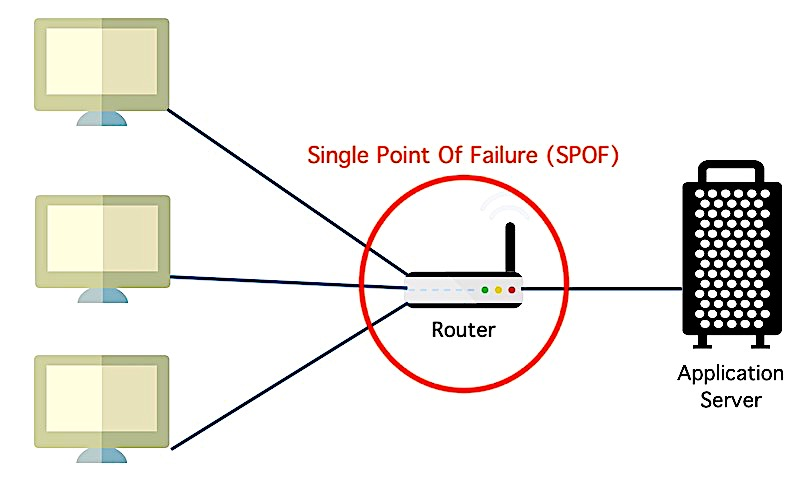
\includegraphics[width=10cm]{spof.jpg}
\caption{Exemplo de um \ac{SPOF}}
\end{figure}

\chapter{Replicação de estado em Sistemas Distribuídos}
\section{Atomicity Consistency Isolation Durability}
\ac{ACID} é um conceito em \ac{SGBD} que identifica um conjunto de propriedades padrão usadas para garantir a fiabilidade de uma determinada base de dados.


\subsection{Transações ACID}
O acesso a diversos itens de dados num sistema distribuído é normalmente acompanhado de transações que têm de preservar as propriedades \ac{ACID}:
\begin{itemize}
    \item \textbf{A}: Atomicidade
    \item \textbf{C}: Consistência
    \item \textbf{I}: Isolamento
    \item \textbf{D}: Durabilidade
\end{itemize}


\subsection{Características da ACID}
\begin{itemize}
    \item \textit{Atomicity} - Numa transação que envolve duas ou mais informações discretas, todas as peças são confirmadas ou nenhuma.
    \item \textit{Consistency} - Uma transação cria um estado de dados novo e válido ou, se ocorrer alguma falha, retorna todos os dados ao seu estado anterior ao início da transação.
    \item \textit{Isolation} - Uma transação em processo e ainda não confirmada deve permanecer isolada de qualquer outra operações.
    \item \textit{Durability} - Os dados comprometidos são salvos pelo sistema de forma que, mesmo em caso de falha e reinicialização do sistema, os dados estejam disponíveis no estado correto.
\end{itemize}

\cleardoublepage

\section{Two Phase Commit Protocol}
O protocolo \ac{2PC} (protocolo de recuperação) divide uma confirmação de \ac{BD} em duas fases para garantir a correção e a tolerância a falhas num sistema de base de dados distribuído. Assume o modelo \textit{fail-stop} (falha-para): os \textit{nodes} que falharem, deixam de estar ativos (param) e não provocam mais erros. 

\subsection{Arquitetura do Protocolo} 
Considere um coordenador de transações que coordena as confirmações dos armazenamentos de base de dados. Como o nome sugere, todo o processo é dividido em duas fases:
\hfill \break

\textbf{Fase \textit{Prepare}:}
\begin{enumerate}
    \item Após cada armazenamento da base de dados (\textit{slave}) ter concluído a sua transação localmente, ele envia uma mensagem \textit{"DONE"} para o coordenador da transação. Uma vez que o coordenador recebe esta mensagem de todos os \textit{slaves}, ele envia aos \textit{slaves} uma mensagem \textit{“PREPARE”}.
    \item Cada \textit{slave} responde à mensagem \textit{“PREPARE”} enviando uma mensagem \textit{“READY”} de volta ao coordenador.
    \item Se um \textit{slave} responder com uma mensagem \textit{“NOT READY”} ou não responder, então o coordenador envia uma mensagem global \textit{“ABORT”} para todos os outros \textit{slaves}. Apenas ao receber uma confirmação de todos os \textit{slaves} de que a transação foi abortada o coordenador considera a transação inteira abortada.
\end{enumerate}


\textbf{Fase \textit{Commit}:}
\begin{enumerate}
    \item Uma vez que o coordenador da transação recebeu a mensagem \textit{“READY”} de todos os \textit{slaves}, ele envia uma mensagem \textit{“COMMIT”} para todos eles, que contém os detalhes da transação que precisa de ser armazenada na base de dados.
    \item Cada \textit{slave} aplica a transação e retorna uma mensagem de confirmação \textit{“DONE”} de volta ao coordenador.
    \item O coordenador considera toda a transação concluída assim que receber uma mensagem \textit{“DONE”} de todos os \textit{slaves}.
\end{enumerate}


\begin{figure}[H]
\center
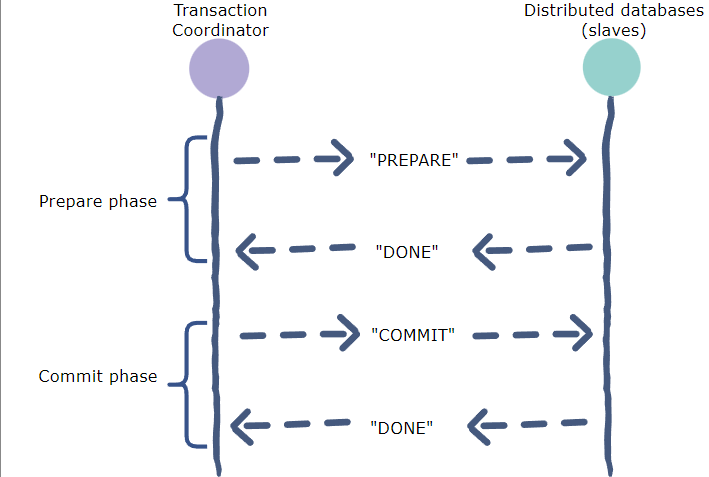
\includegraphics[width=8cm]{2pc.png}
\caption{Funcionamento do Protocolo 2PC}
\end{figure}

Para finalizar, o \ac{2PC}, está relacionado com os princípios já abordados anteriormente, \ac{ACID}, porque este protocolo garante a atomicidade, a consistência, o isolamento e a durabilidade de uma transação.


\section{Base de Dados Distribuídas}
Um sistema de bases de dados distribuídas consiste em múltiplos servidores, cada um responsável pelos seus dados. Estes dados podem ser acedidos utilizando uma rede e, apesar de estarem fisicamente distribuídos, devem apresentar-se ao utilizador logicamente integrados, como se estivessem num único servidor. 

\subsection{Divisão de Base de Dados Distribuídas}
Podemos dizer que Bases de Dados Distribuídas se encontram divididas em dois sistemas:

\begin{enumerate}
    \item Sistemas Homogéneos: todos os \textit{nodes}  usam o mesmo \ac{SGBD} mas os dados estão armazenados em várias \ac{BD}.
    \item Sistemas Heterogéneos: cada \textit{node} utiliza um \ac{SGBD} diferente onde partilham \ac{BD} pré existentes com mesmo modelo de dados ou modelos de dados diferentes. 
\end{enumerate}

\subsection{Vantagens e Desvantagens de Base de Dados Distribuídas}
\begin{itemize}
    \item Vantagens: Uma das vantagens para utilizar Base de Dados Distribuídas é pelo fato, como o nome indica, de ser de natureza distribuída. Ou seja, geograficamente se uma organização tiver várias sedes espalhadas pelo país faz sentido utilizar uma base de dados distribuída, pois vai espelhar a estrutura da organização, vai implicar que cada sede tenho o seu próprio servidor.
    Resumidamente, existe maior segurança, partilha de dados e autonomia local, desempenho melhorado (em relação ás \ac{BD}), fiabilidade/disponibilidade e é mais vantajoso para representar várias organizações.
    \item Desvantagem: Ao contrário da vantagem dada, não se justifica ter vários servidores espalhados quando uma organização possui geograficamente as suas delegações/sedes umas ao lado das outras. Neste caso faz mais sentido ter uma solução cliente/servidor.
    Resumidamente, tem custos de desenvolvimento de Software, maior possibilidade de erros no software, aumento da carga de processamento e aumento da complexidade da coordenação dos \textit{nodes}.
\end{itemize}

\cleardoublepage
\section{Sistema de Gestão de Base de Dados}
Um \ac{SGBD} é o software que gere o armazenamento, manipulação e pesquisa dos dados existentes na \ac{BD}, funcionando como uma interface entre as aplicações e os dados necessários para a execução dessas aplicações.\\*
\indent Exemplos \ac{SGBD}: Microsoft SQL Server, Oracle Server, MariaDB, MySQL, entre outros.


\begin{figure}[H]
\center
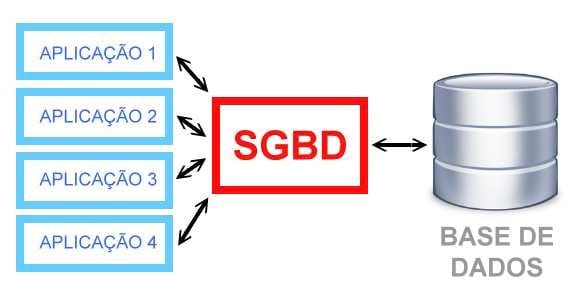
\includegraphics[width=8cm]{sgbd.jpg}
\caption{Arquitetura \ac{SGBD}}
\end{figure}

\subsection{Requisitos fundamentais de um SGBD}
\begin{itemize}
    \item Segurança: proteção da \ac{BD} contra acessos não autorizados;
    \item Integridade: validação de operações que coloquem em risco a consistência dos dados;
    \item Controlo de concorrência nos acessos: coordenação da partilha dos dados pelos vários utilizadores
    \item Recuperação de falhas: restaurar a integridade da \ac{BD} depois da ocorrência de uma falha. Mecanismos de recuperação (fundamentalmente baseados em redundância): backups, \textit{transaction logging} (ficheiro \textit{transaction log}, dados para repor as últimas transações).
\end{itemize}

\cleardoublepage
\section{Replicação de dados}
A replicação é a técnica de duplicar dados em vários \textit{nodes} diferentes. Para tornar a replicação segura existe um conjunto de razões para a duplicação dos dados, que passo a citar:

\begin{itemize}
    \item Prevenção contra falhas: a falha de um \textit{node} que contenha dados importantes ao sistema não compromete, necessariamente, o seu funcionamento;
    \item Redução da transferência de dados: há uma maior probabilidade de os dados estarem disponíveis localmente ou mais perto do \textit{node} que os requisita. Isto resulta na redução dos custos de transferência;
    \item Paralelismo: os pedidos à \ac{BD} podem ser processados por vários \textit{nodes} em paralelo, o que vai existir um maior desempenho.
\end{itemize}


Como não falamos só de vantagens, neste caso também existe desvantagens e neste cenário de replicação uma das desvantagens é a necessidade de manter uma coerência total do sistema. A coerência total do sistema implica que quando a informação num \textit{node} é atualizada, as suas réplicas também devem ser atualizadas, o que aumenta o \textit{overhead} do sistema (custos de atualização e necessidade de algoritmos complexos para a execução de transações).\\*
\indent Dentro do sistema, conforme as atualizações propagadas, a replicação pode ser \textbf{síncrona} (ocorre em tempo real e é preferida para sistemas com objetivos de baixo tempo de recuperação que não podem perder dados), \textbf{assíncrona} (replicação lenta e projetado para trabalhar em distâncias e requer menos largura de banda).\\*

Para concluir, quando os dados têm de estar permanentemente atualizados, é preferível recorrer à replicação síncrona. Caso contrário, deve-se utilizar a replicação assíncrona por ter melhores tempos de resposta e até é possível indicar intervalos de tempo para as atualizações.\\*

A replicação traz mais benefícios quando os dados são lidos muitas vezes pelos servidores remotos, mas poucas vezes atualizados, devido à carga adicional que é colocada sobre o sistema para manter as réplicas consistentes. 

\cleardoublepage

\section{Conclusão sobre o item (2) do enunciado}
O protocolo \ac{2PC} assegura que a propriedade da atomicidade da transação é respeitada. Caso exista um \textit{Abort} de um dos \textit{nodes} a transação falha.\\*
\indent O \ac{2PC} pode ficar inoperante devido à falha de um dos \textit{nodes} durante o processo. Uma transação inoperante não é desejável porque continua a manter os \textit{locks} dos recursos de que necessita para a sua transação, impedindo que outras transações que precisem desses mesmos recursos os possam obter.\\*
\indent O objetivo das técnicas de tolerâncias de falhas nas Base de Dados Distribuídas é garantir que não há perda/corrupção de dados.\\*
\indent O \ac{SGBD} é responsável por tudo, guardar os dados no disco rígido, manter em memória os dados mais acedidos, ligar dados e metadados (dados sobre outros dados), disponibilizar uma interface para programas e utilizadores. Isto são algumas das vantagens de um \ac{SGBD} mas como temos visto também tem as suas desvantagens. Trabalhar com três \ac{SGBD} implica utilizar mais do que um utilizador e não pode prejudicar nenhum deles. O controlo de acesso irá garantir a integridade dos dados com a possibilidade de configurar níveis de acesso a cada utilizador (segurança). 


\subsection{Falhas que podem ocorrer no 2PC}
\begin{itemize}
    \item Falhas nos \textit{nodes};
    \item Falhas na rede;
    \item Falhas de Software;
    \item Falha do coordenador.
\end{itemize}

\subsection{Desvantagens do 2PC}
Como já foi referido atrás, uma das desvantagens é o protocolo \ac{2PC} ser demasiado restritivo, basta que um dos \textit{nodes} falhe ou fique inoperável e os restantes \textit{nodes} efetuam um \textit{rollback}. Uma segunda desvantagem é se existir uma falha após a primeira fase (fase antes do envio das instruções de \textit{commit} ou \textit{abort}, todas as sub-transações ficam bloqueadas (num estafo de espera ativa mantendo os \textit{locks} que possuíam.

Para resolver estes problemas (Desvantagens acima descritas) foi criado o protocolo \ac{3PC}. Um protocolo não muito usado devido ao elevado tráfego que necessitava. O \ac{3PC} é um protocolo semelhante ao \ac{2PC} mas com um passo adicional intermédio \textit{Pre-Commit},que confirma se todos os \textit{nodes} estão em condições de finalização.


\chapter{Arquiteturas de Software Modernas}
\section{Instalação Proxmox}

Inicialmente foram criados os vários servidores proxmox (DD1, DD2, DD3) e para isso fica registado passo a passo a instalação.\\

Passo 1: "Create a new virtual machine".
\begin{figure}[H]
\center
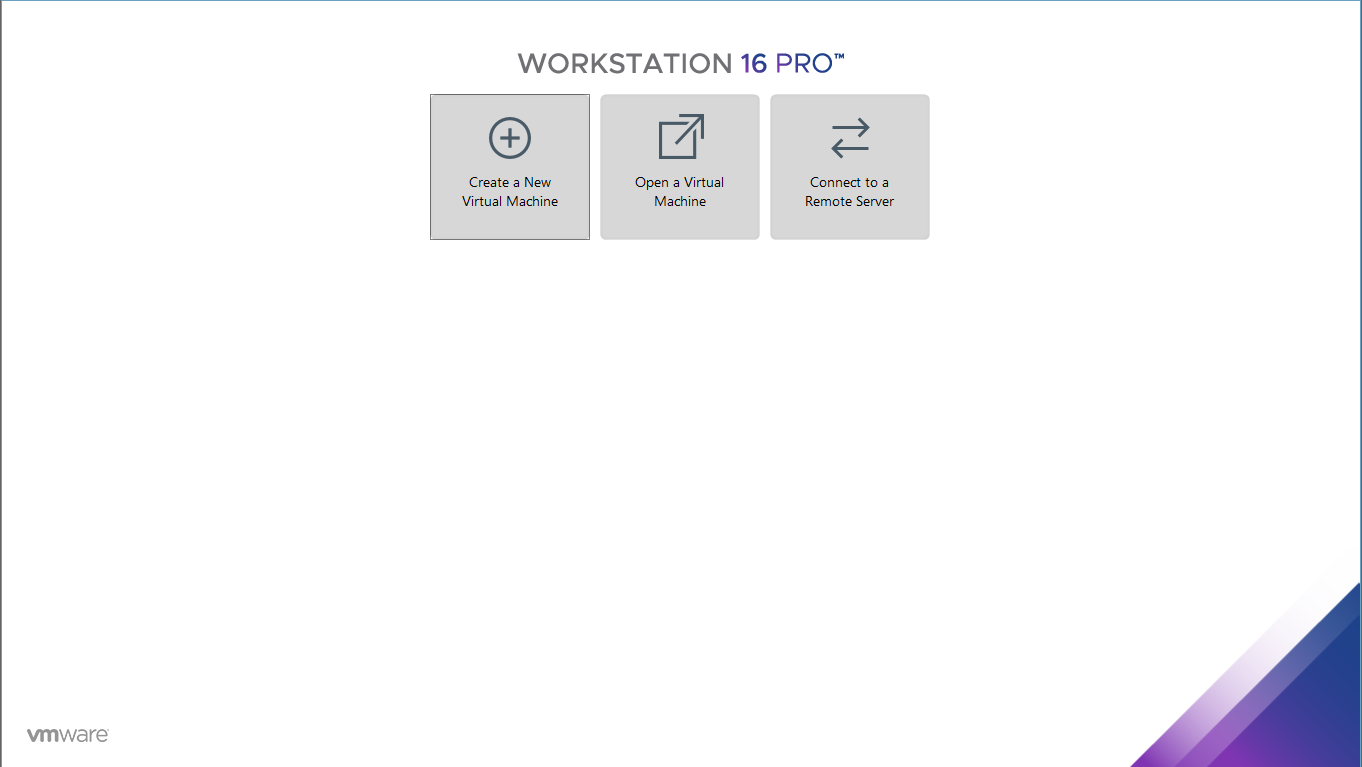
\includegraphics[width=13cm]{Screenshot_1.png}
\caption{Create a new virtual machine}
\end{figure}

\newpage
Passo 2: Aqui é escolha pessoal, eu escolhi "Typical".
\begin{figure}[H]
\center
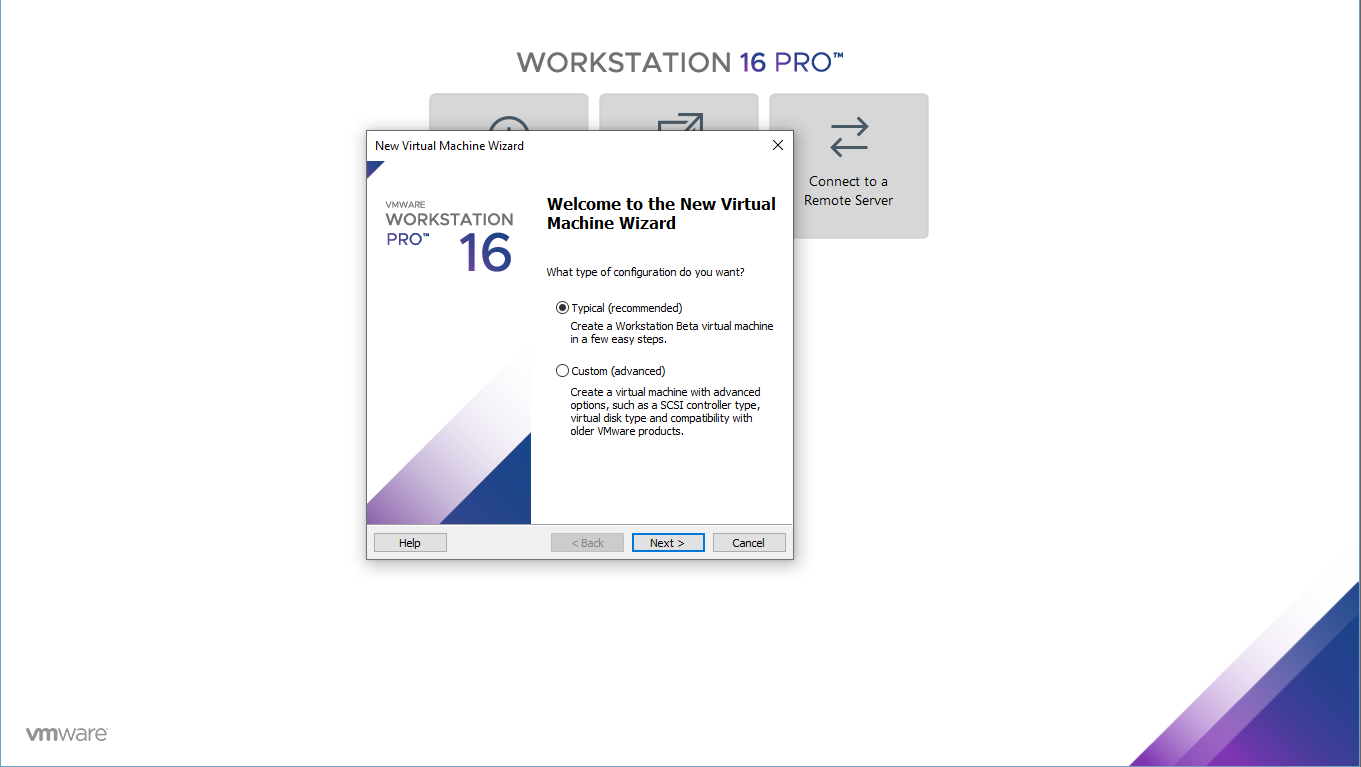
\includegraphics[width=13cm]{Screenshot_2.png}
\caption{Tipo de configuração}
\end{figure}

Passo 3: Escolhi instalar o Sistema Operativo mais tarde.
\begin{figure}[H]
\center
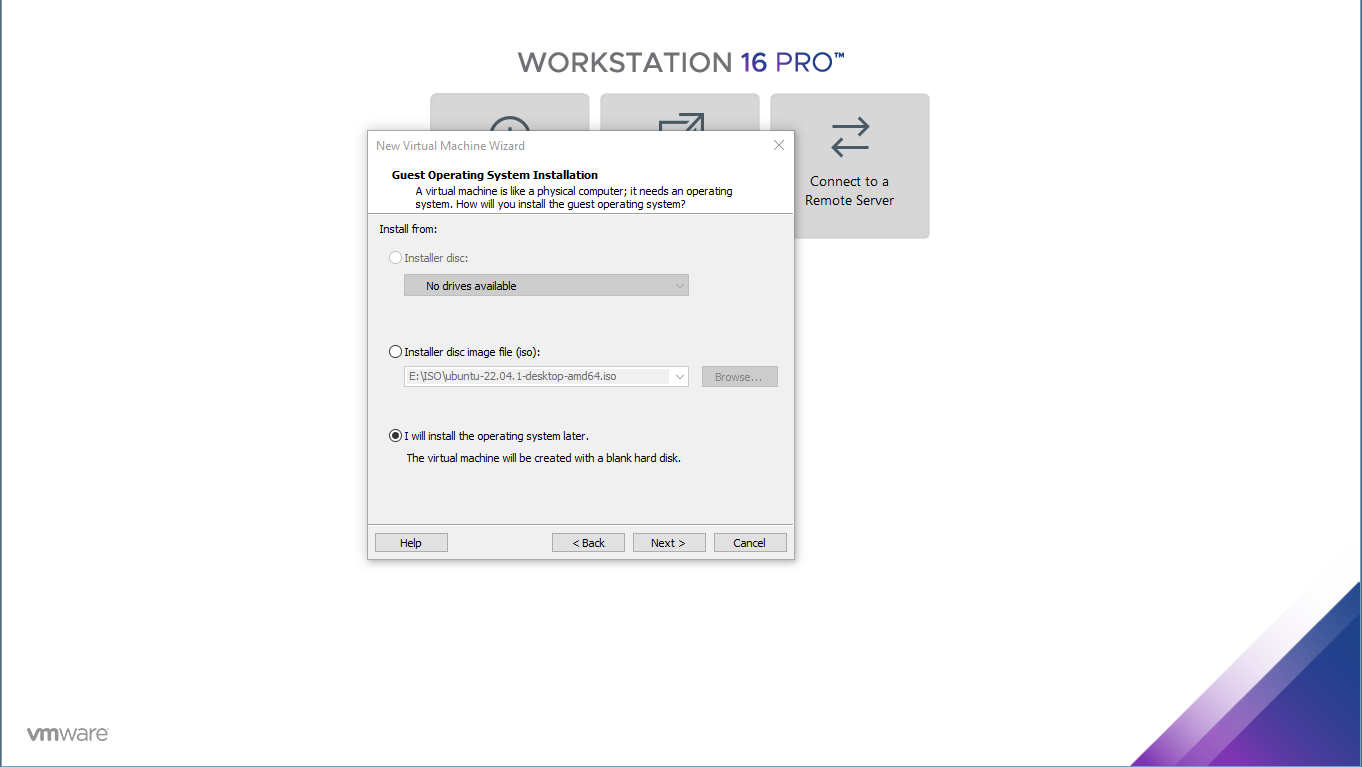
\includegraphics[width=13cm]{Screenshot_3.png}
\caption{Install the Operating System later}
\end{figure}

\newpage
Passo 4: Por predefinição deixei ficar as opções dadas uma vez que o proxmox é baseado em Linux.
\begin{figure}[H]
\center
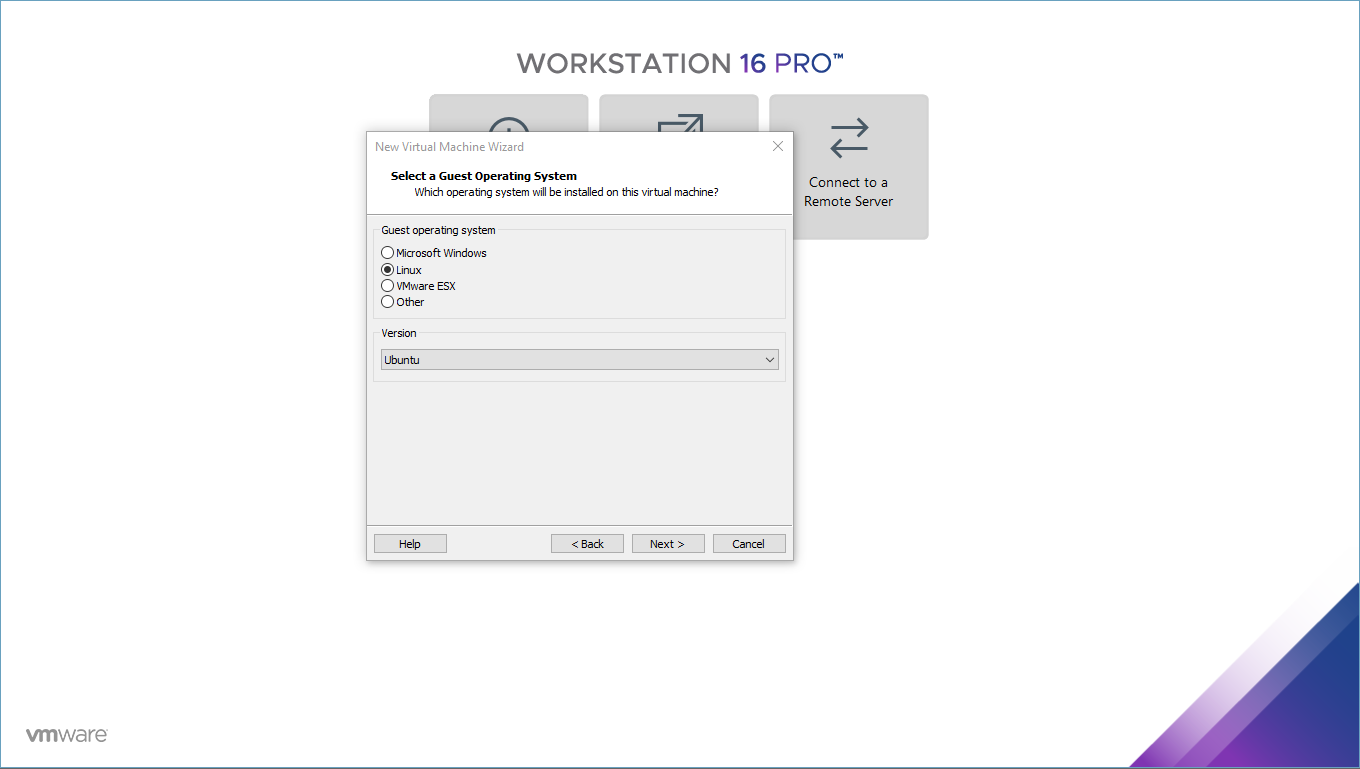
\includegraphics[width=13cm]{Screenshot_4.png}
\caption{Tipo Sistema Operativo}
\end{figure}

Passo 5: Escolher o nome (Proxmox) para a \ac{VM} e a localização. Neste caso utilizei um disco externo de 1TB.
\begin{figure}[H]
\center
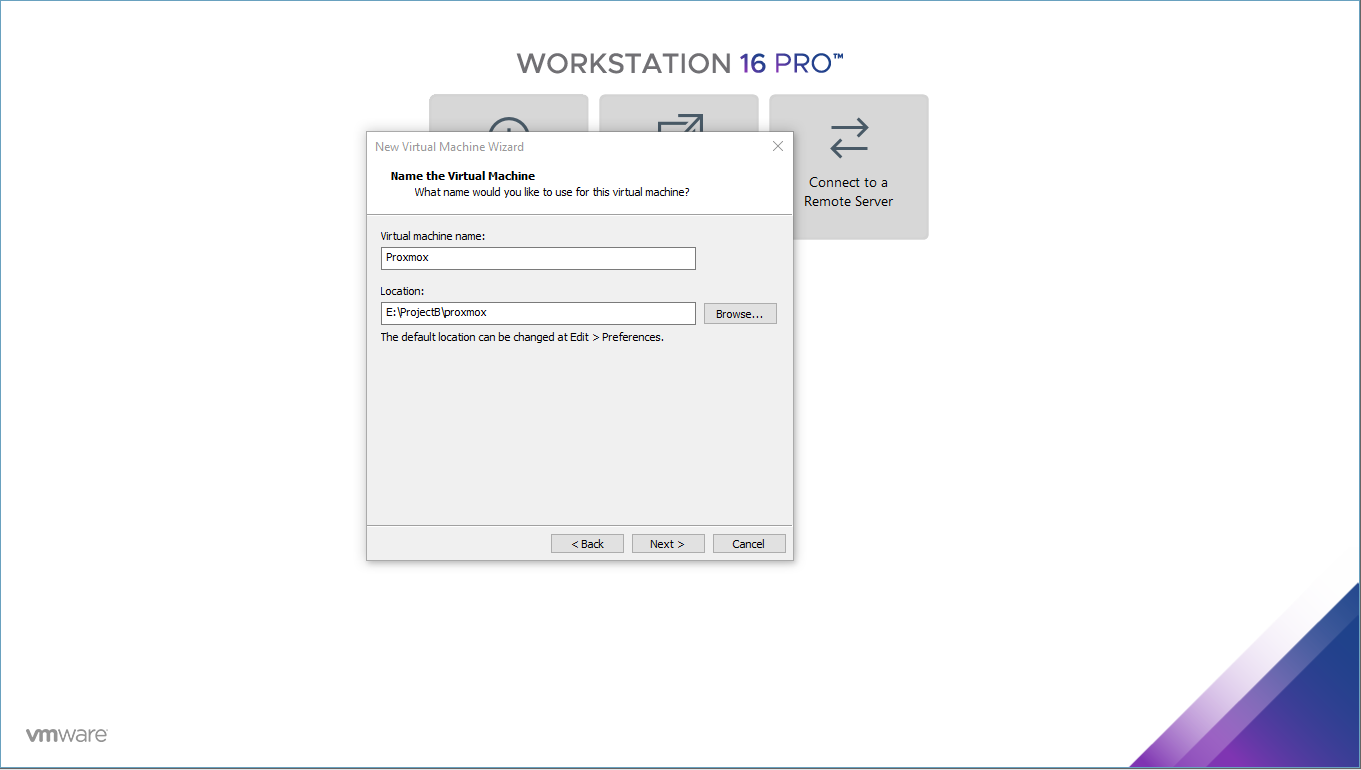
\includegraphics[width=13cm]{Screenshot_5.png}
\caption{Nome e localização da \ac{VM}}
\end{figure}

\newpage
Passo 6: Definir o tamanho do disco para a \ac{VM}. Neste caso foi 120Gb.
\begin{figure}[H]
\center
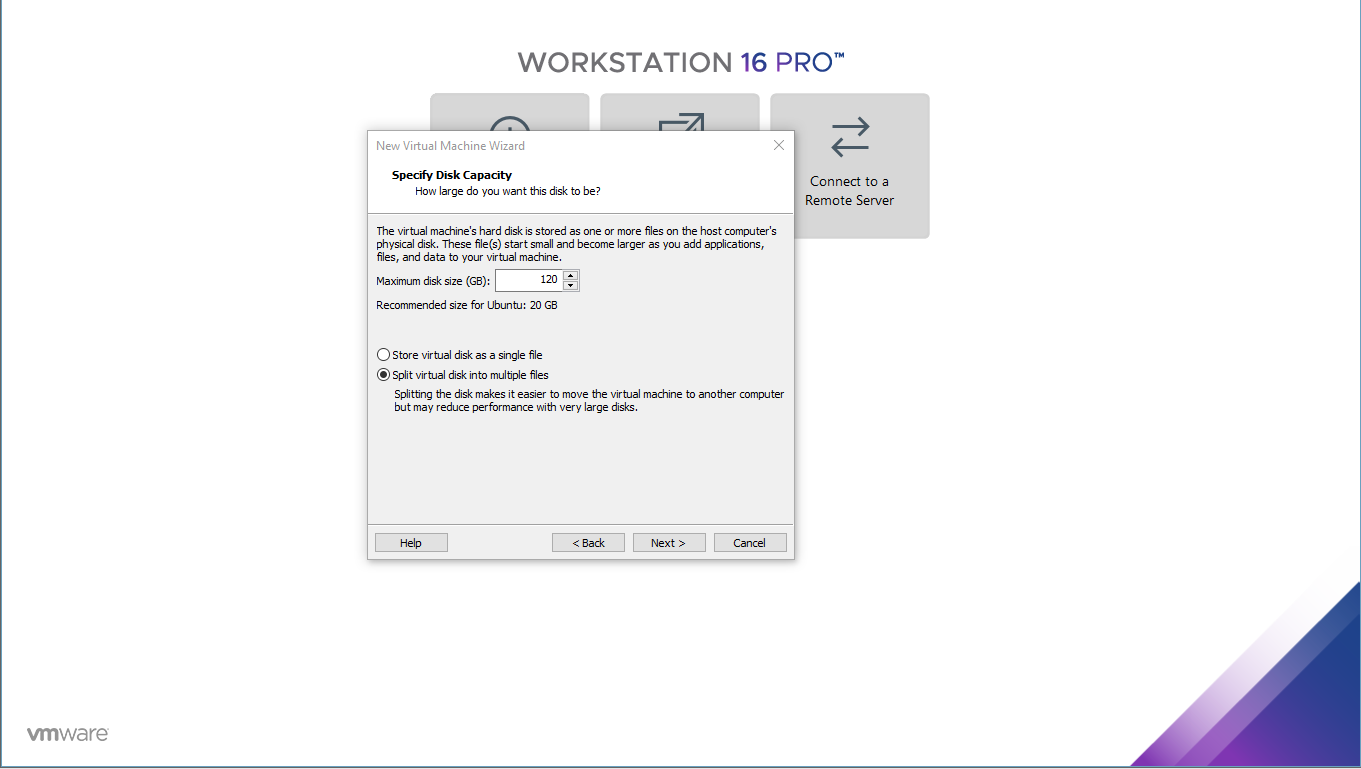
\includegraphics[width=13cm]{Screenshot_6.png}
\caption{Tamanho Disco \ac{VM}}
\end{figure}

Passo 7: Resumo da configuração e finalização.
\begin{figure}[H]
\center
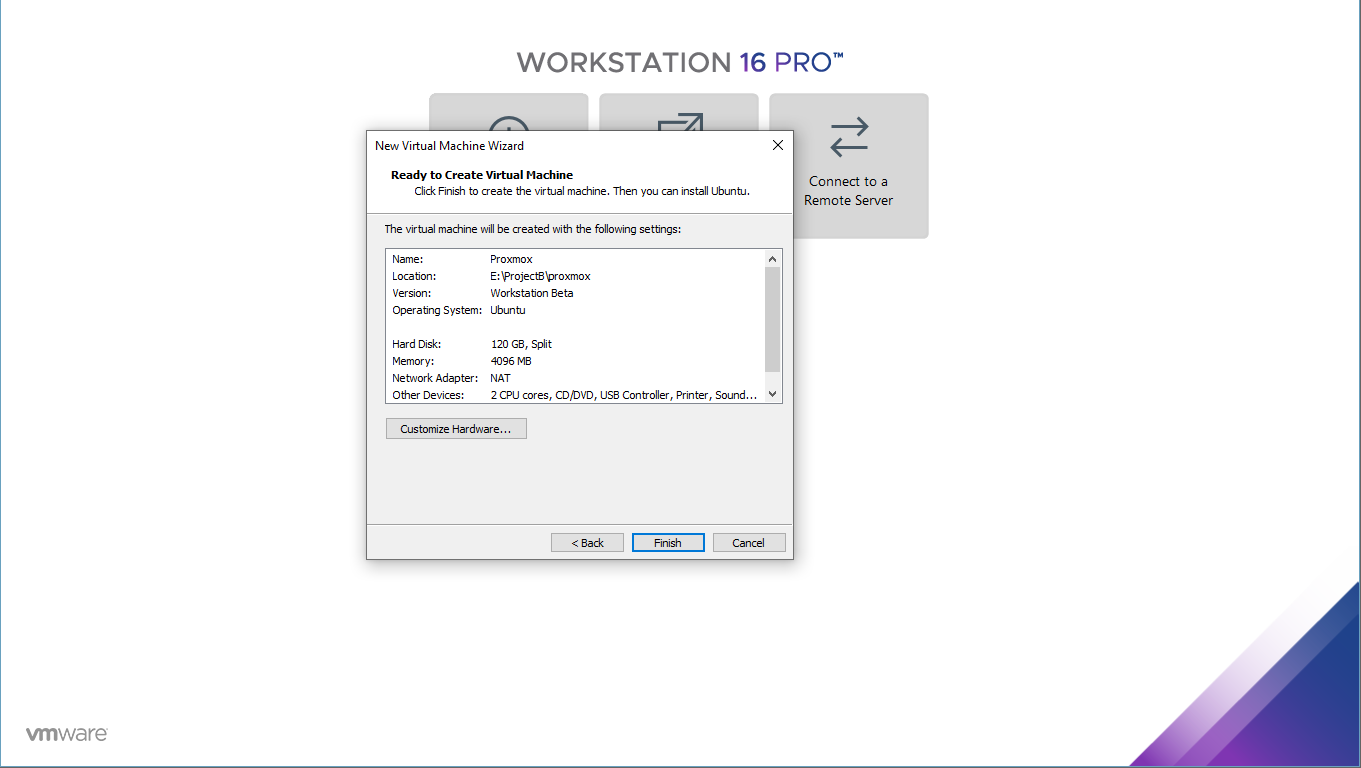
\includegraphics[width=13cm]{Screenshot_7.png}
\caption{Finalização}
\end{figure}

\newpage
Passo 8: Nas propriedades da \ac{VM}, inseri a \ac{ISO} do proxmox em "\ac{CD/DVD} (\ac{SATA})".
\begin{figure}[H]
\center
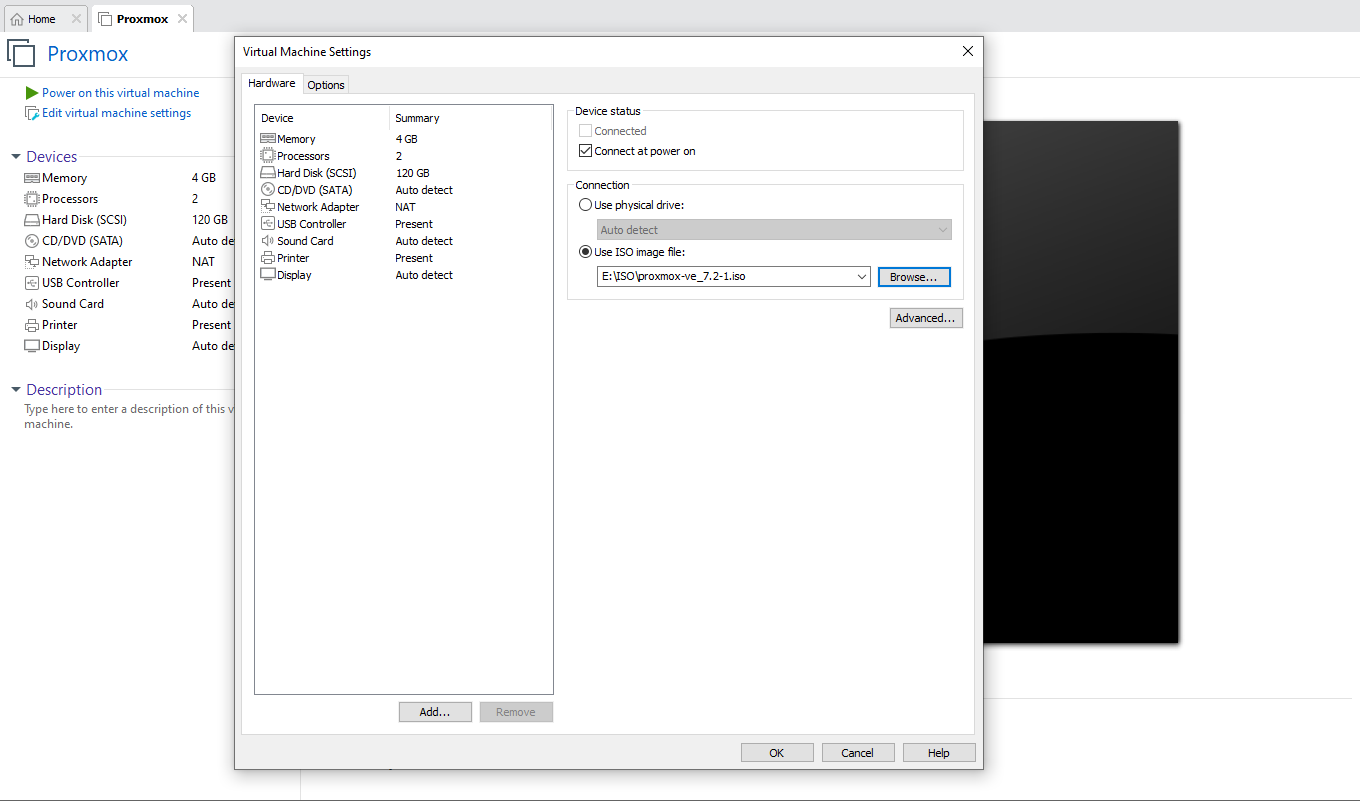
\includegraphics[width=13cm]{Screenshot_8.png}
\caption{Inserir \ac{ISO}}
\end{figure}

Passo 9: Ainda nas propriedades da \ac{VM}, a placa de rede tem de estar em modo \textit{bridge}.
\begin{figure}[H]
\center
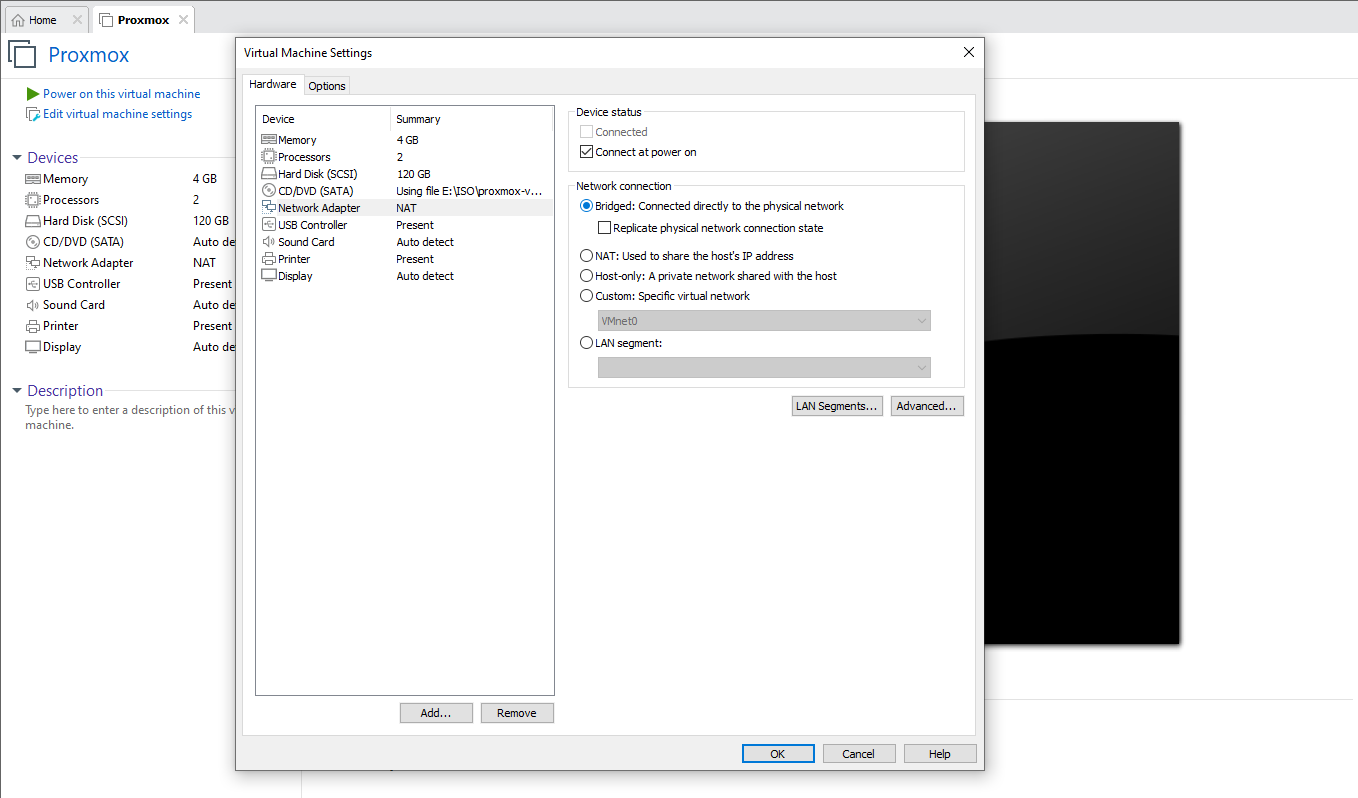
\includegraphics[width=13cm]{Screenshot_9.png}
\caption{Placa de rede}
\end{figure}

\newpage
Passo 10: Depois de alterar algumas configurações iniciais, podemos iniciar a \ac{VM} e iniciar a instalação.
\begin{figure}[H]
\center
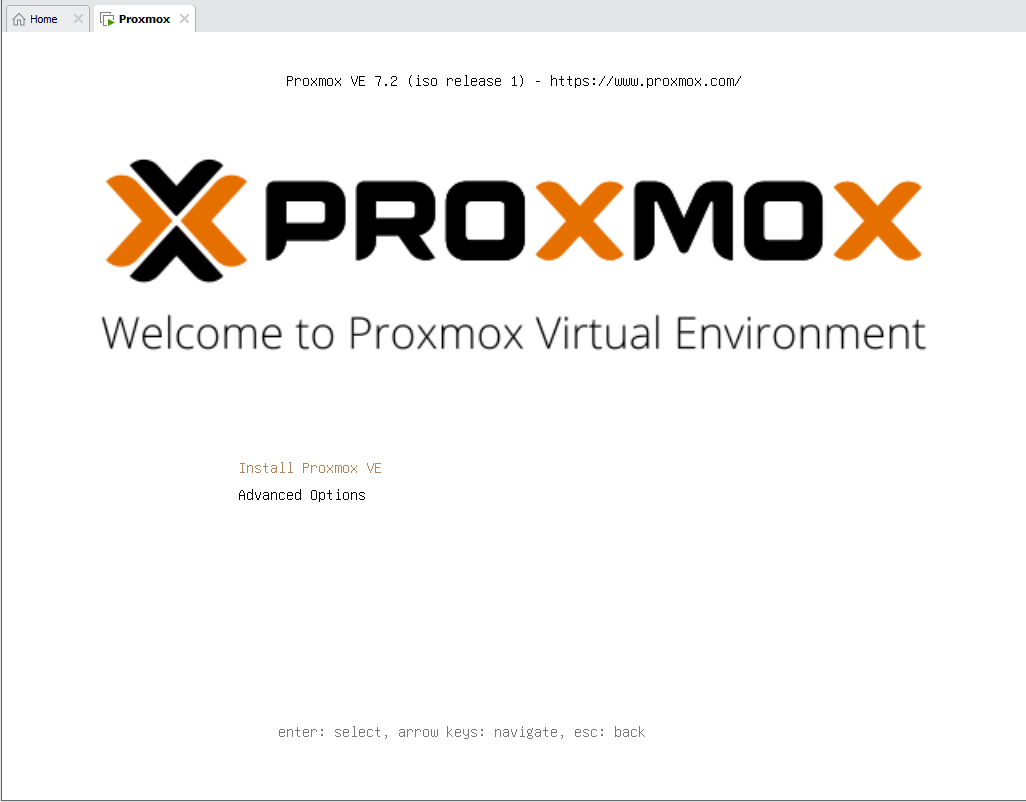
\includegraphics[width=13cm]{Screenshot_10.png}
\caption{Inicialização da \ac{VM}}
\end{figure}

Passo 11: Aceitar os termos e condições do proxmox.
\begin{figure}[H]
\center
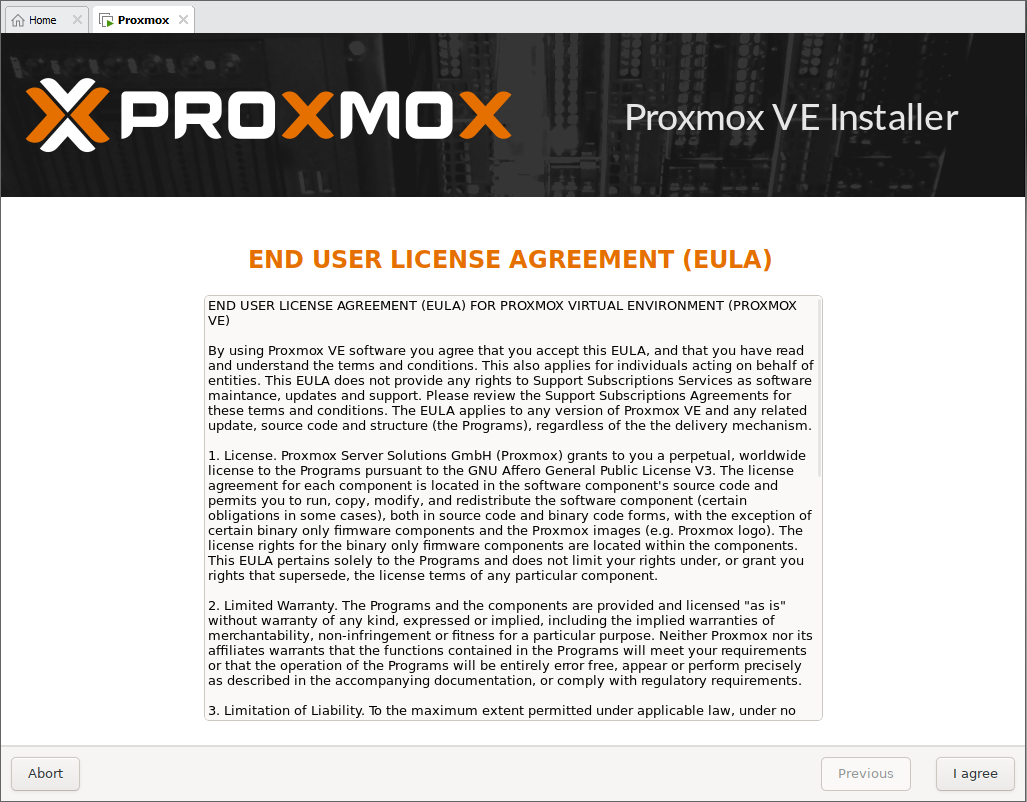
\includegraphics[width=13cm]{Screenshot_11.png}
\caption{Termos e condições}
\end{figure}

\newpage
Passo 12: Escolha do disco para a instalação do servidor. No meu caso estou a usar um disco \ac{HDD} de 1TB e os 120Gb foi a "partição" que criamos inicialmente na criação da \ac{VM}.
\begin{figure}[H]
\center
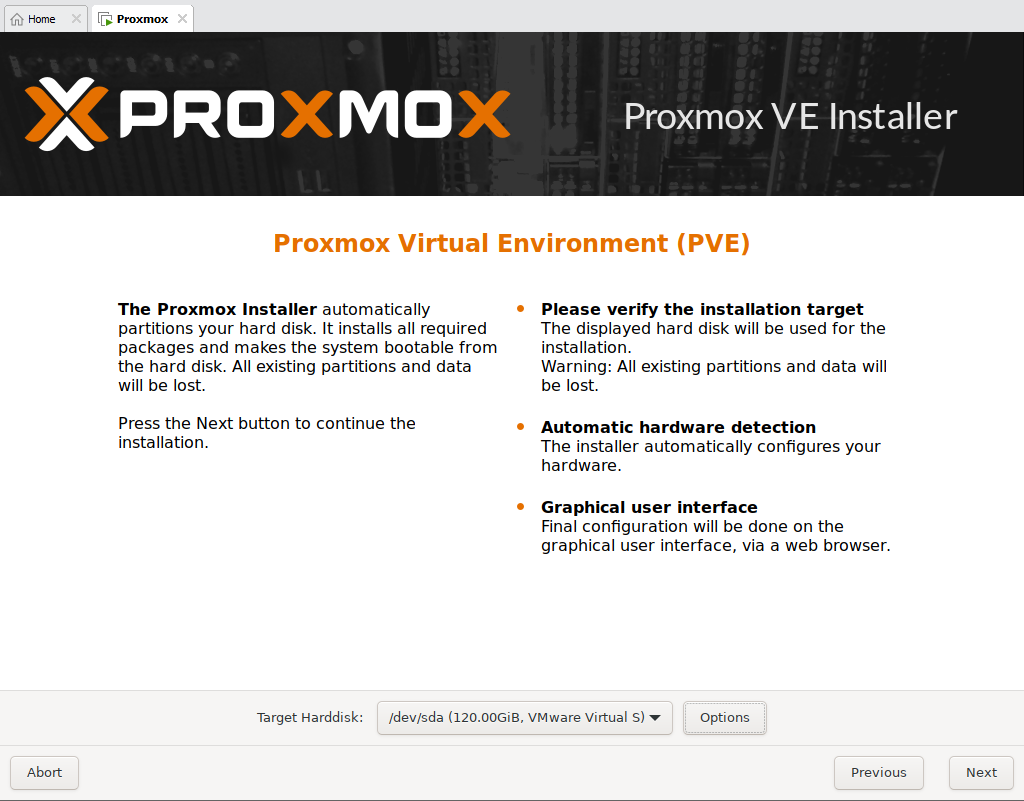
\includegraphics[width=13cm]{Screenshot_14.png}
\caption{Escolha do disco rígido}
\end{figure}

O File System usado foi \textit{ext4}.
\begin{figure}[H]
\center
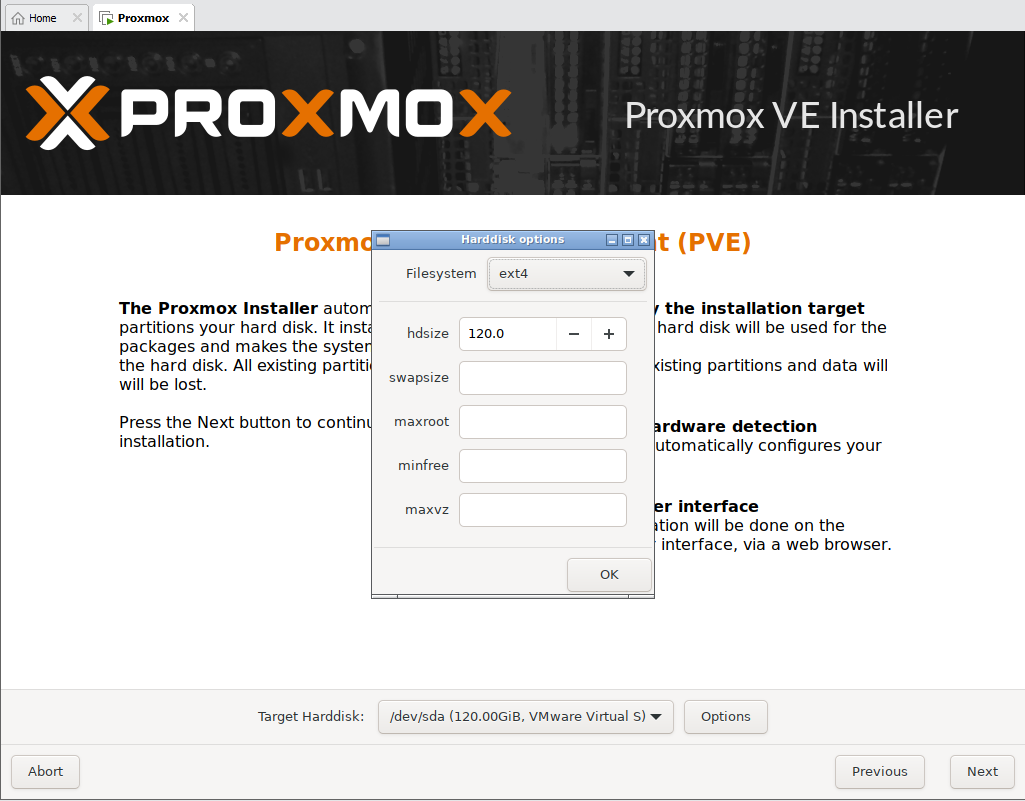
\includegraphics[width=13cm]{Screenshot_12.png}
\caption{File System}
\end{figure}

\newpage
Passo 13: Escolha do país, fuso horário e \textit{layout} do teclado.
\begin{figure}[H]
\center
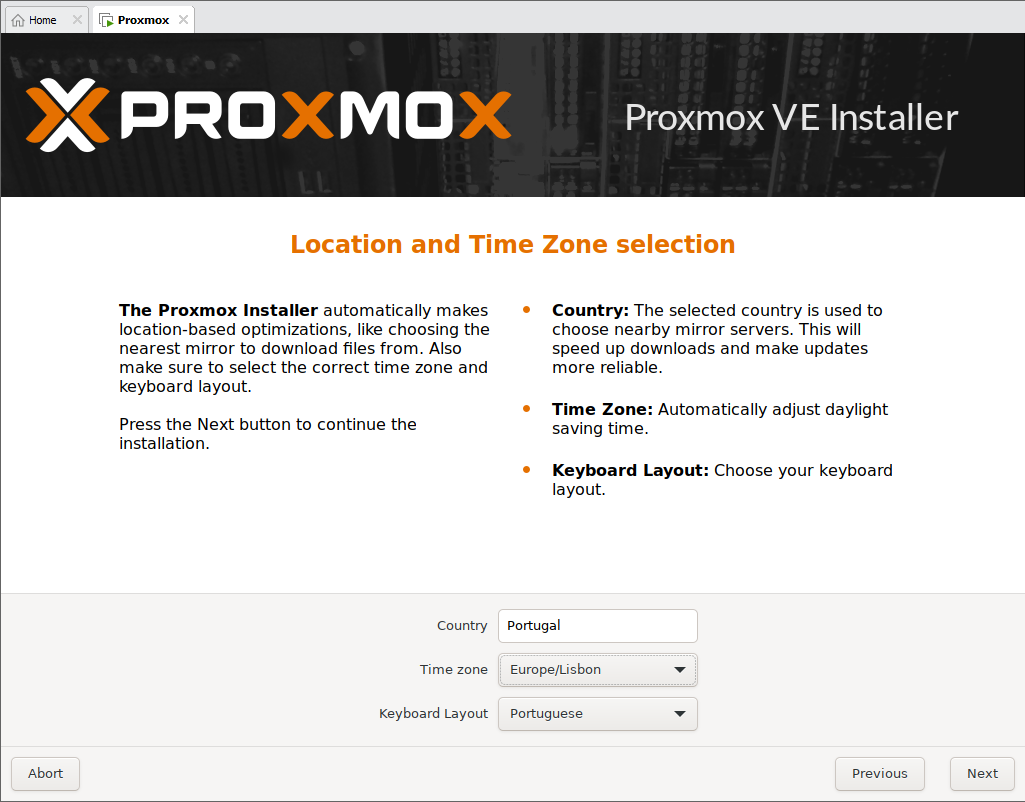
\includegraphics[width=13cm]{Screenshot_15.png}
\caption{Localização e fuso horário}
\end{figure}

Passo 14: Definir uma \textit{password} de administração e \textit{email}.
\begin{figure}[H]
\center
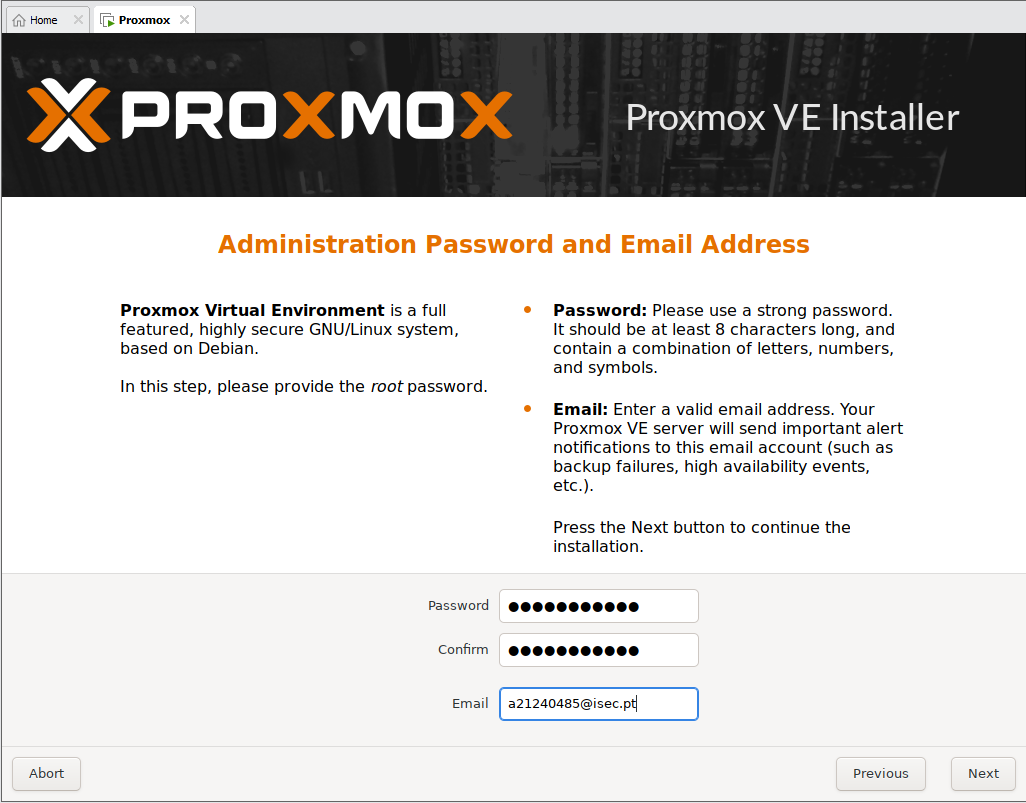
\includegraphics[width=13cm]{Screenshot_16.png}
\caption{Password de Administração e Email}
\end{figure}

\newpage
Passo 15: Para a configuração da Rede de Gestão foi definido a placa de rede (ens33), hostoname (DD1.VM), \ac{IP} (192.168.1.129/24), gateway e \ac{DNS}.
\begin{figure}[H]
\center
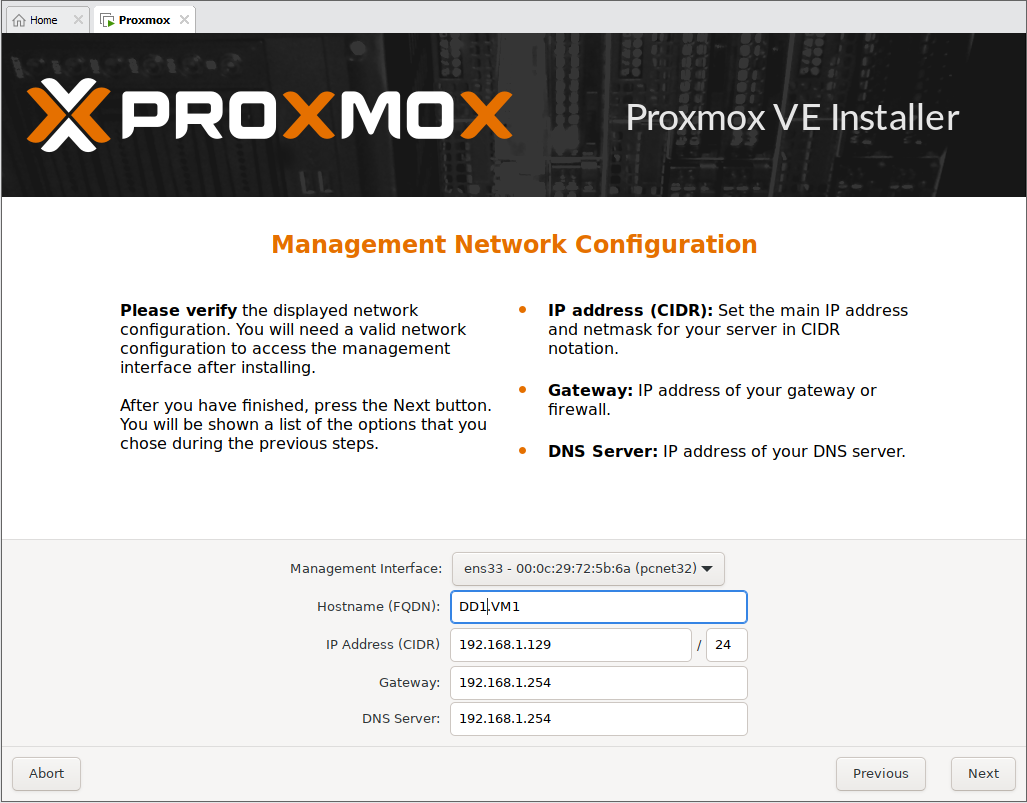
\includegraphics[width=13cm]{Screenshot_17.png}
\caption{Configuração da Rede de Gestão}
\end{figure}

Passo 16: Aqui podemos verificar o resumo das opções de instalação e prosseguir com a instalação.
\begin{figure}[H]
\center
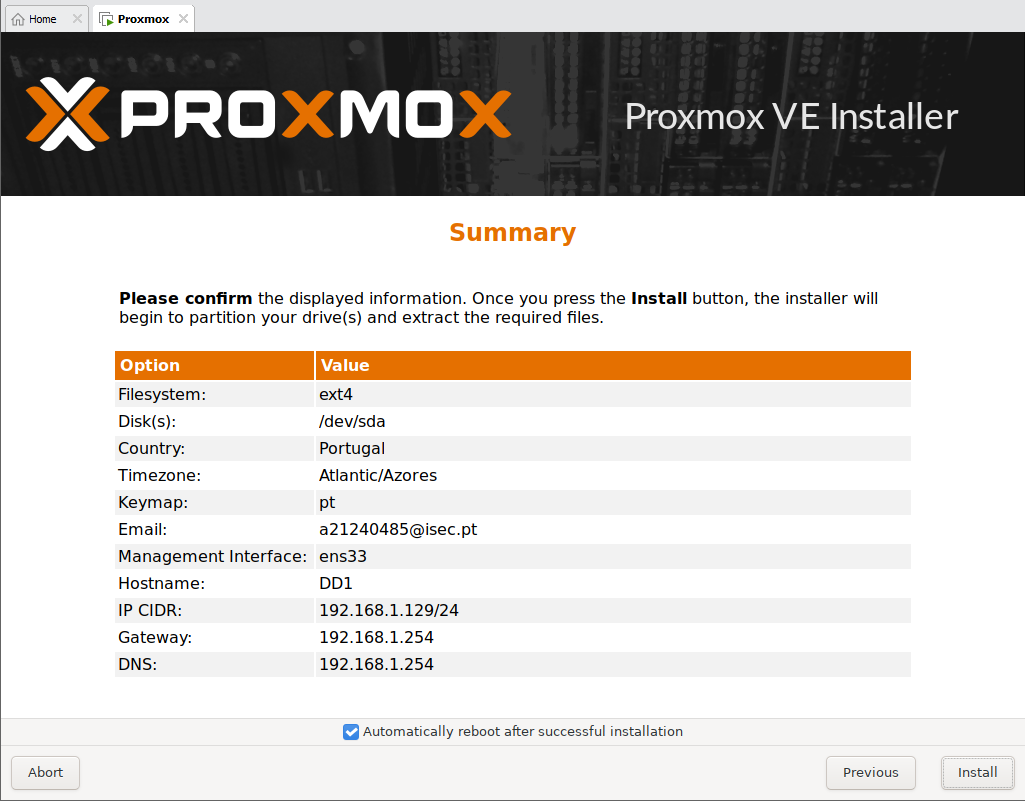
\includegraphics[width=13cm]{Screenshot_18.png}
\caption{Resumo da Instalação}
\end{figure}

\newpage
Passo 17: Instalação do proxmox.
\begin{figure}[H]
\center
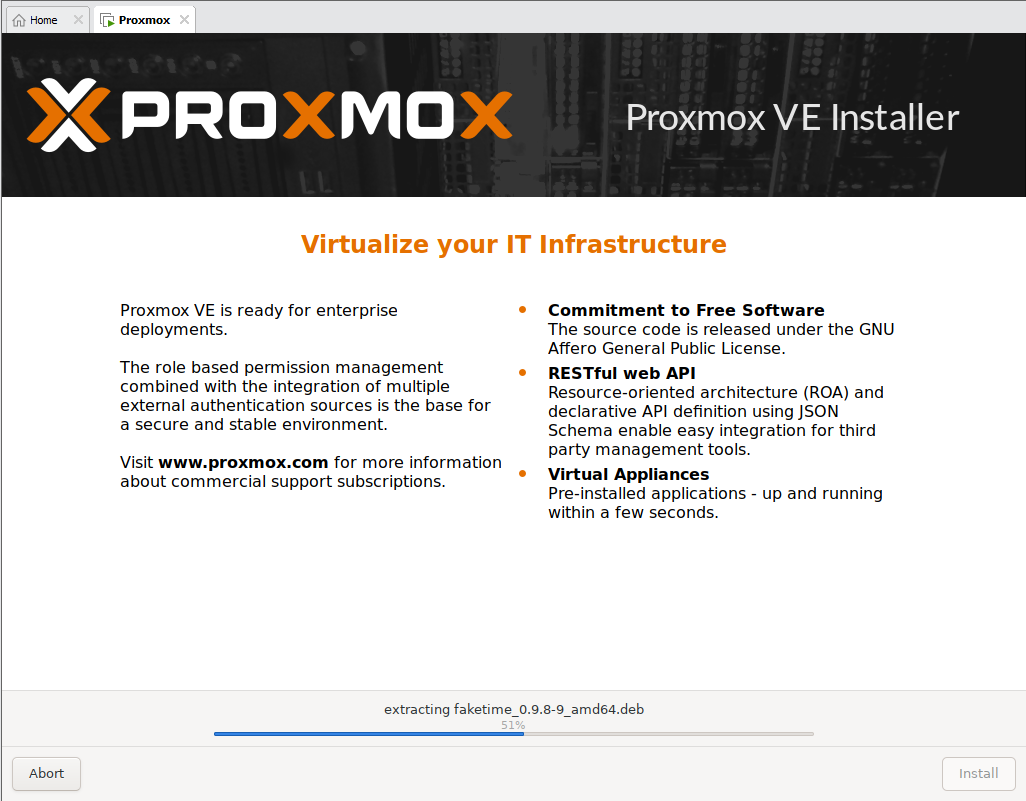
\includegraphics[width=13cm]{Screenshot_19.png}
\caption{Instalação}
\end{figure}

Passo 18: Após a instalação do proxmox é necessário reiniciar o servidor e de seguida fica pronto a ser utilizado. Na tela de apresentação do servidor é apresentado o endereço para poder aceder ao servidor proxmox através da interface web.
\begin{figure}[H]
\center
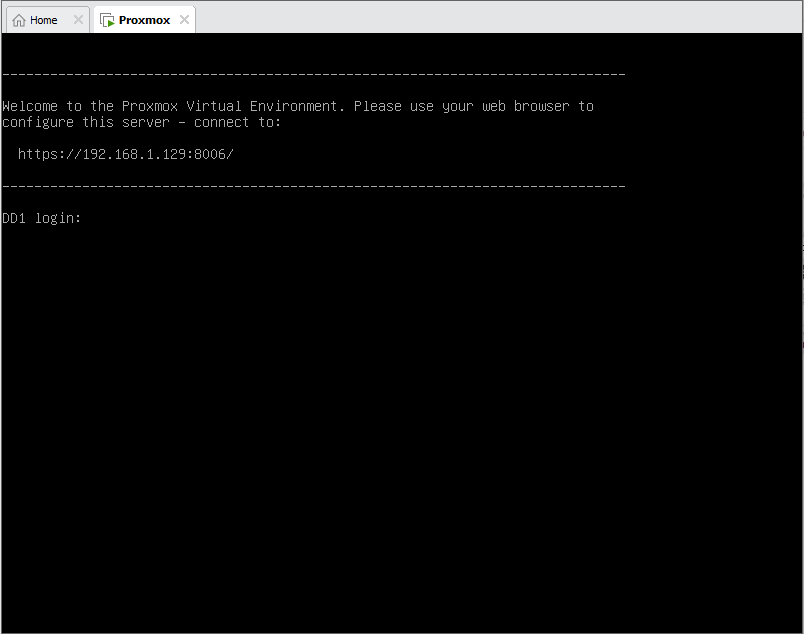
\includegraphics[width=13cm]{Screenshot_20.png}
\caption{\ac{PVE} login}
\end{figure}

\newpage
Passo 19: Depois de verificar o \ac{PVE} login no passo anterior, o mesmo nos indica o endereço para poder aceder à interface web. Num browser à escolha apenas basta conectar ao \ac{IP} do servidor mais a porta 8006 do proxmox. 
\begin{verbatim}https://192.168.1.129:8006\end{verbatim}
\begin{figure}[H]
\center
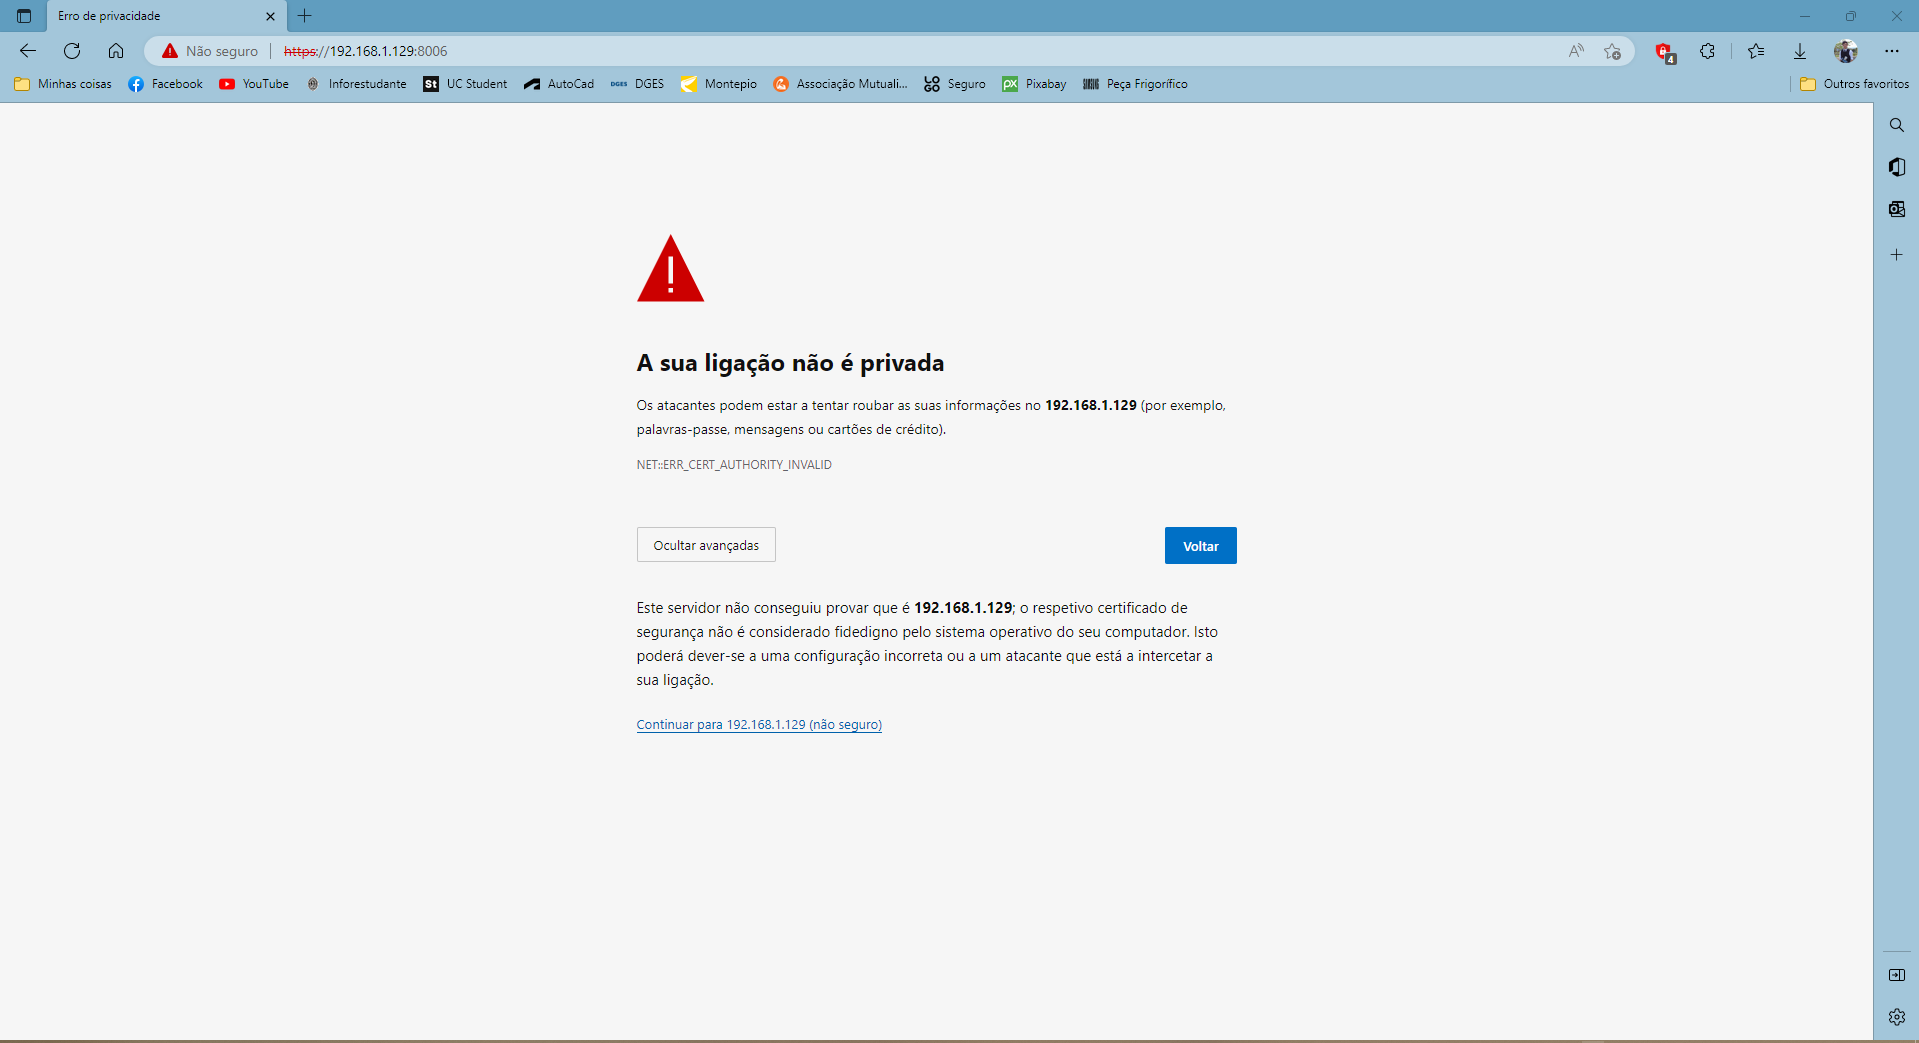
\includegraphics[width=14cm]{Screenshot_21.png}
\caption{Ligação Não Privada}
\end{figure}

O browser vai mostrar o erro de que a ligação não é privada porque não existe um certificado válido mas prosseguimos carregando em: \textbf{"Continuar para 192.168.1.129 (não seguro)"}. De seguida passamos para a tela inicial de login do servidor proxmox.

\begin{figure}[H]
\center
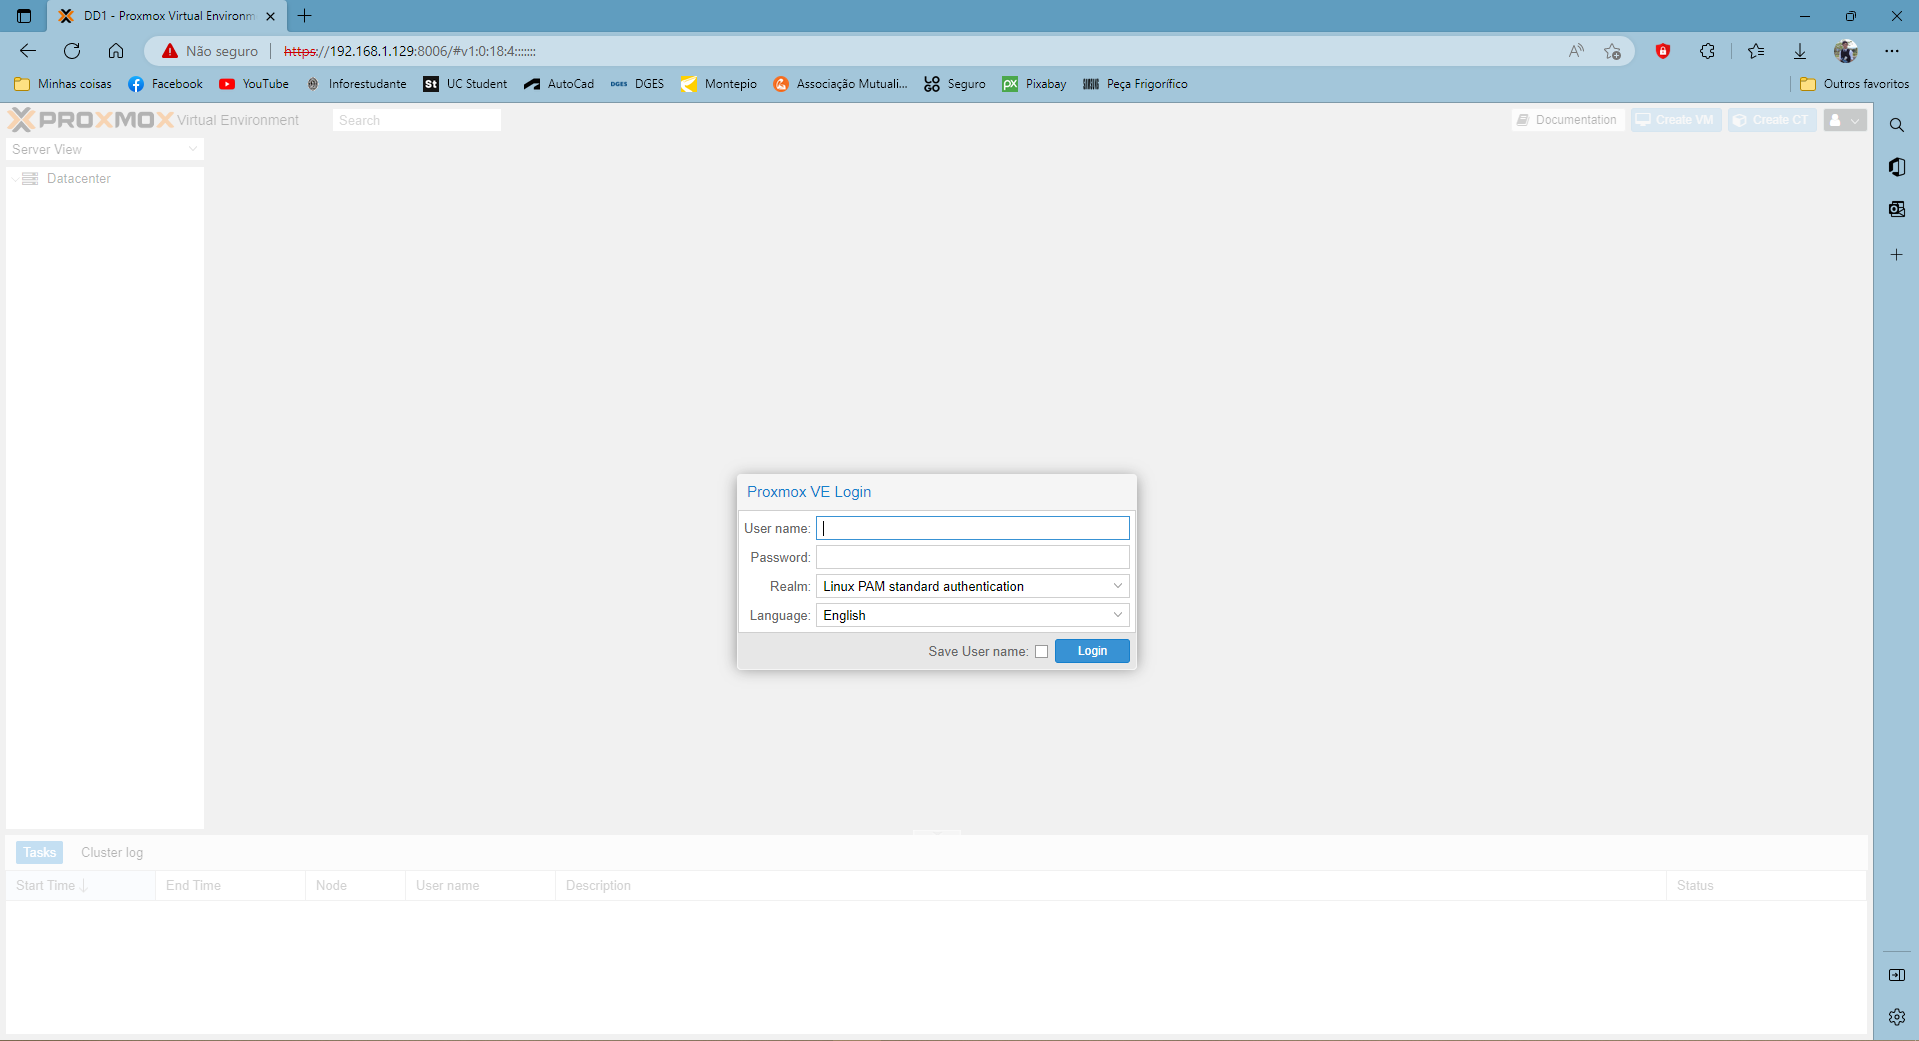
\includegraphics[width=14cm]{Screenshot_22.png}
\caption{\ac{PVE} login}
\end{figure}

O \textit{username} por predefinição é \textit{root} e a \textit{password} foi definida no passo 14.

\newpage
Passo 20: Depois da autenticação temos acesso completo ao servidor proxmox via interface web. 
\begin{figure}[H]
\center
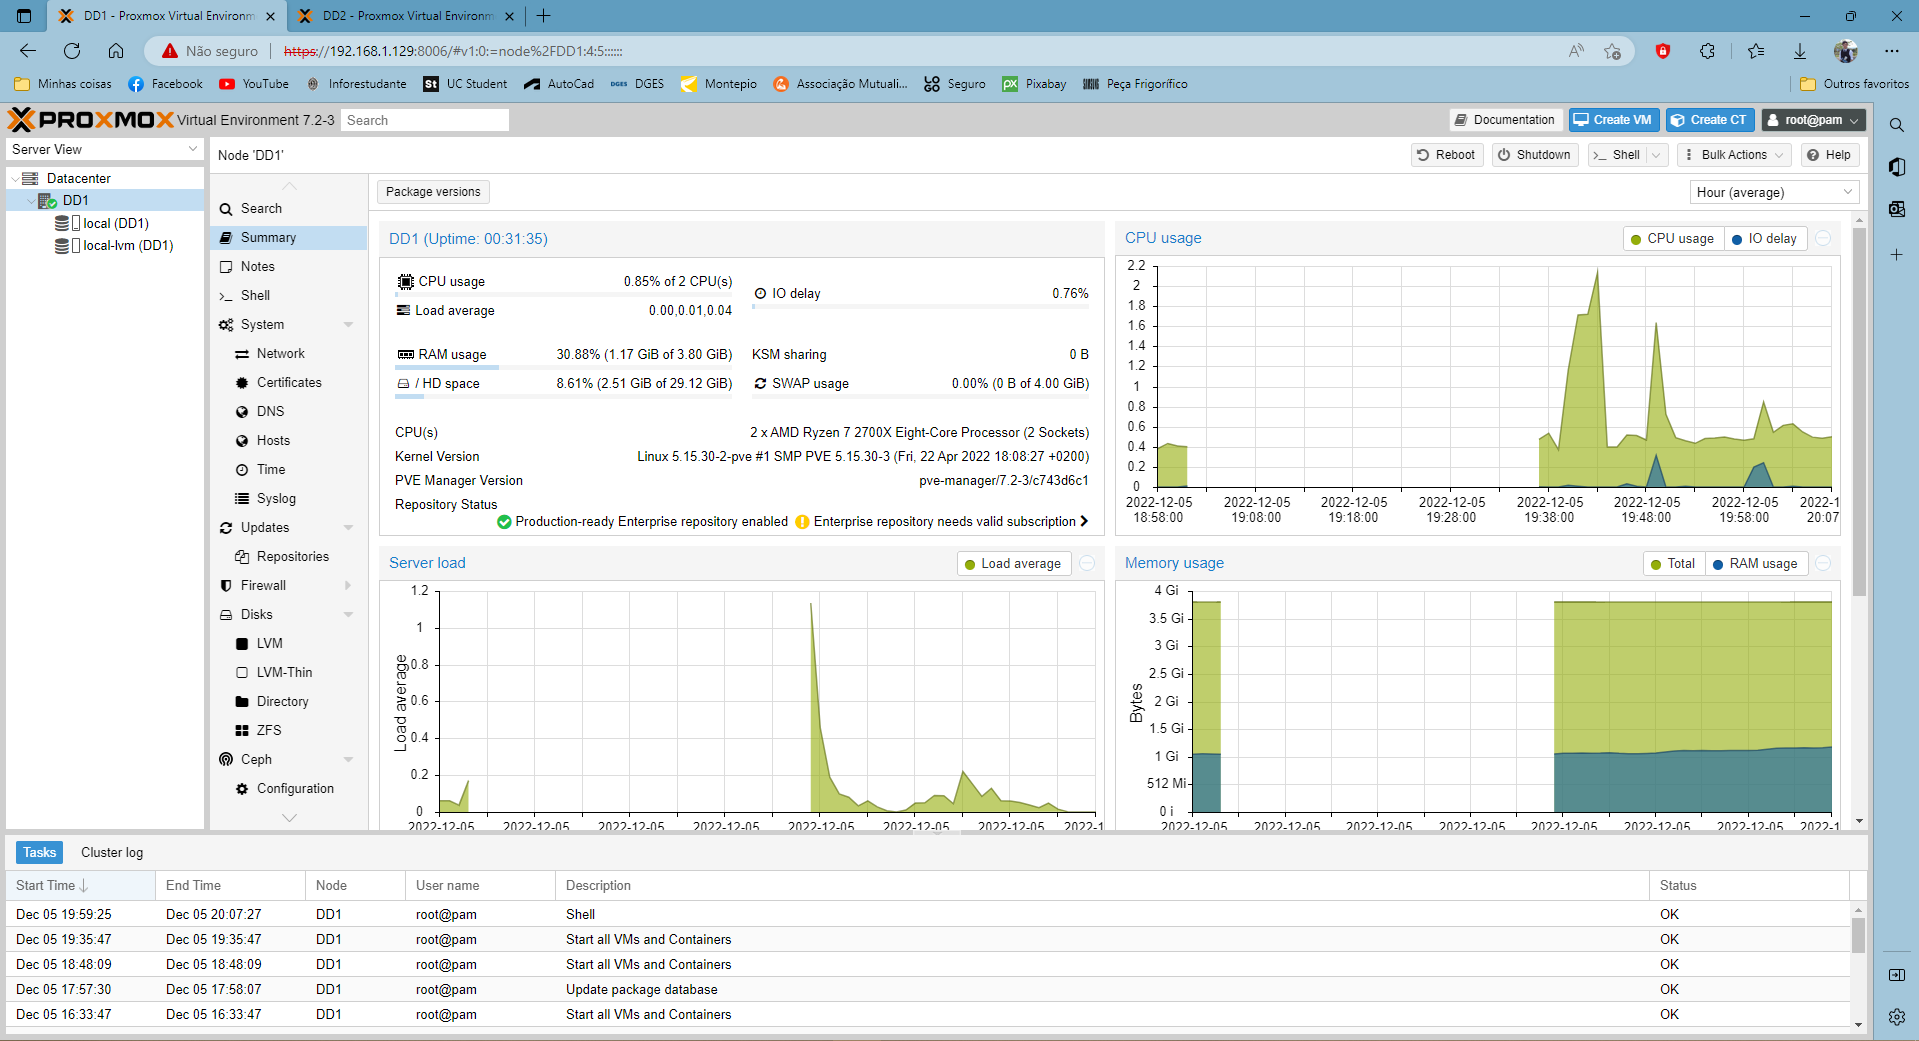
\includegraphics[width=14cm]{Screenshot_24.png}
\caption{Summary DD1}
\end{figure}

O objetivo é a construção de um \textit{cluster} e para isso é preciso no mínimo 3 servidores. De seguida foi adicionado mais 2 servidores proxmox seguindo todos os passos anteriores.
Depois de repetir todos os passos anteriores o objetivo é ter 3 servidores proxmox a funcionar em simultâneo (DD1, DD2 e DD3) no VMWare:

\begin{figure}[H]
\center
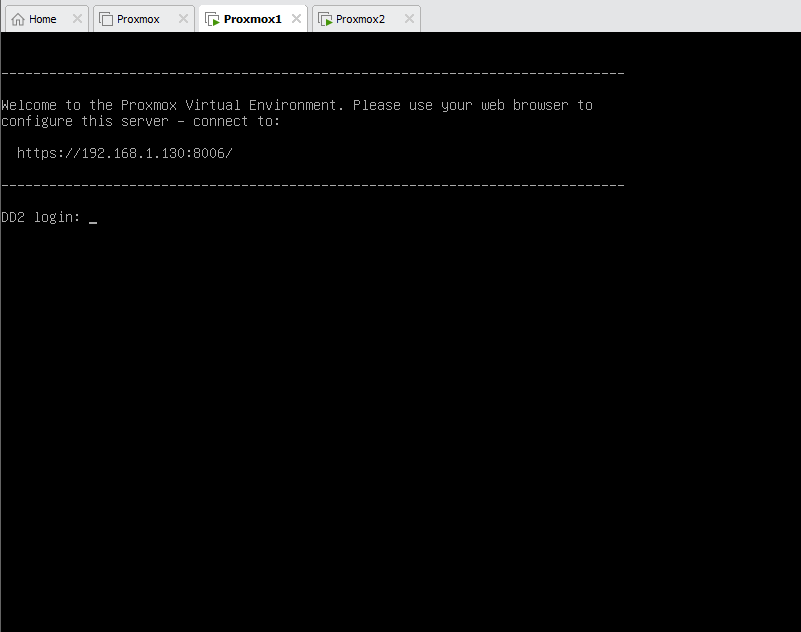
\includegraphics[width=14cm]{Screenshot_26.png}
\caption{Servidor proxmox DD2}
\end{figure}

\newpage
\begin{figure}[H]
\center
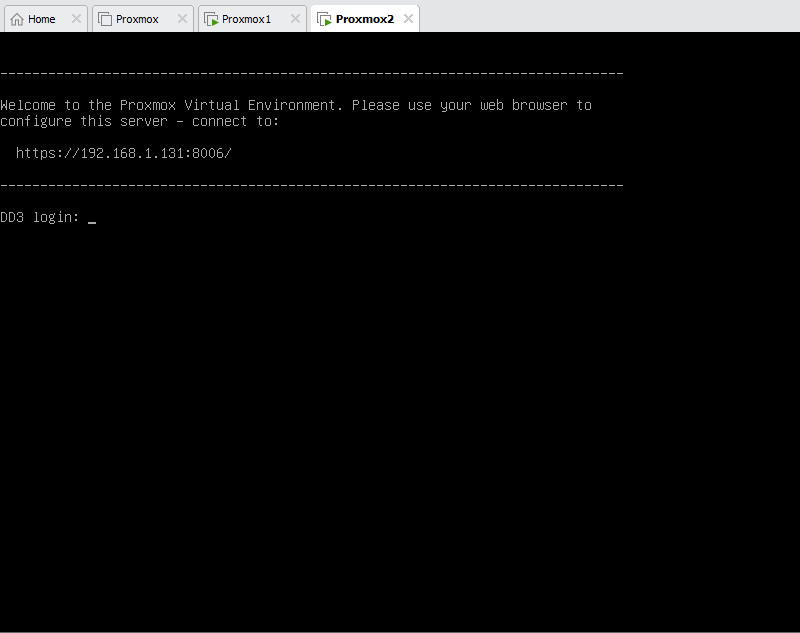
\includegraphics[width=14cm]{Screenshot_27.png}
\caption{Servidor proxmox DD3}
\end{figure}

\newpage
\section{Configuração Ficheiro Hosts}
O ficheiro "hosts" é usado principalmente para resolver nomes de host localmente, sem precisar de uma consulta ao servidor \ac{DNS}. Ele também pode ser usado para bloquear o acesso a sites específicos, redirecionando o nome de host para um endereço \ac{IP} inválido. Além disso, é frequentemente usado em ambientes de desenvolvimento para mapear nomes de host para endereços IP locais.

Desta forma prosseguimos com a configuração do ficheiro "hosts" em cada servidor. O ficheiro "hosts" encontra-se na seguinte diretoria:
\begin{verbatim}/etc/hosts\end{verbatim}

Esta configuração foi realizada através da linha de comandos do servidor proxmox e para isso basta efetuar o \textit{login} no servidor com o \textit{username} \textbf{root} e a \textit{password}.\\

Passo 1: Como foi dito anteriormente, é preciso ter acesso ao servidor proxmox e efetuar o \textit{login}.  
\begin{figure}[H]
\center
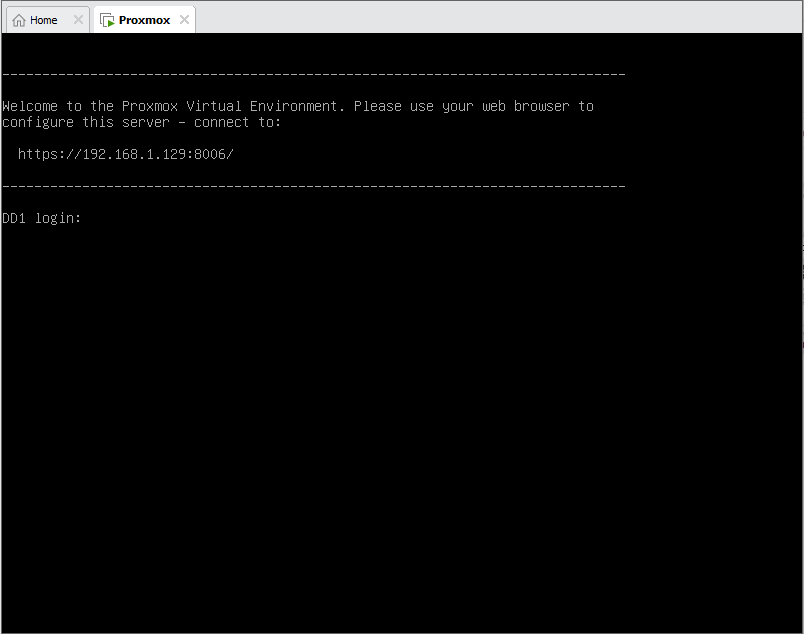
\includegraphics[width=14cm]{Screenshot_20.png}
\caption{Login Servidor DD1}
\end{figure}

\newpage
Passo 2: Depois de efetuar o \textit{login}, com recurso ao editor de texto nano do linux, configuramos o ficheiro "hosts":
\begin{verbatim}nano /etc/hosts\end{verbatim}

No servidor 1, Proxmox (DD1), foi adicionado o servidor 2 e 3.
\begin{verbatim}192.168.1.130 DD2.VM2 DD2\end{verbatim}
\begin{verbatim}192.168.1.131 DD3.VM3 DD3\end{verbatim}

\begin{figure}[H]
\center
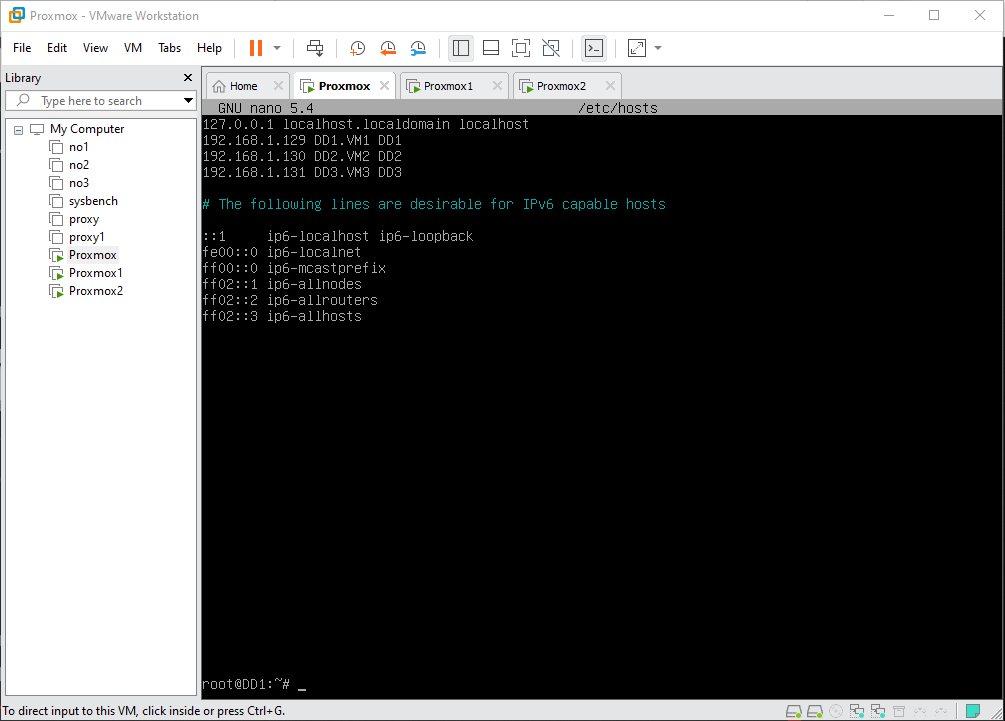
\includegraphics[width=14cm]{Screenshot_135.png}
\caption{Configuração do ficheiro Hosts no servidor 1}
\end{figure}

Nos restantes servidores basta seguir os passos anteriores e adicionar os servidores corretos.

\newpage
Servidor 2, Proxmox1 (DD2), foi adicionado o servidor 1 e 3.
\begin{verbatim}192.168.1.129 DD1.VM1 DD1\end{verbatim}
\begin{verbatim}192.168.1.131 DD3.VM3 DD3\end{verbatim}

\begin{figure}[H]
\center
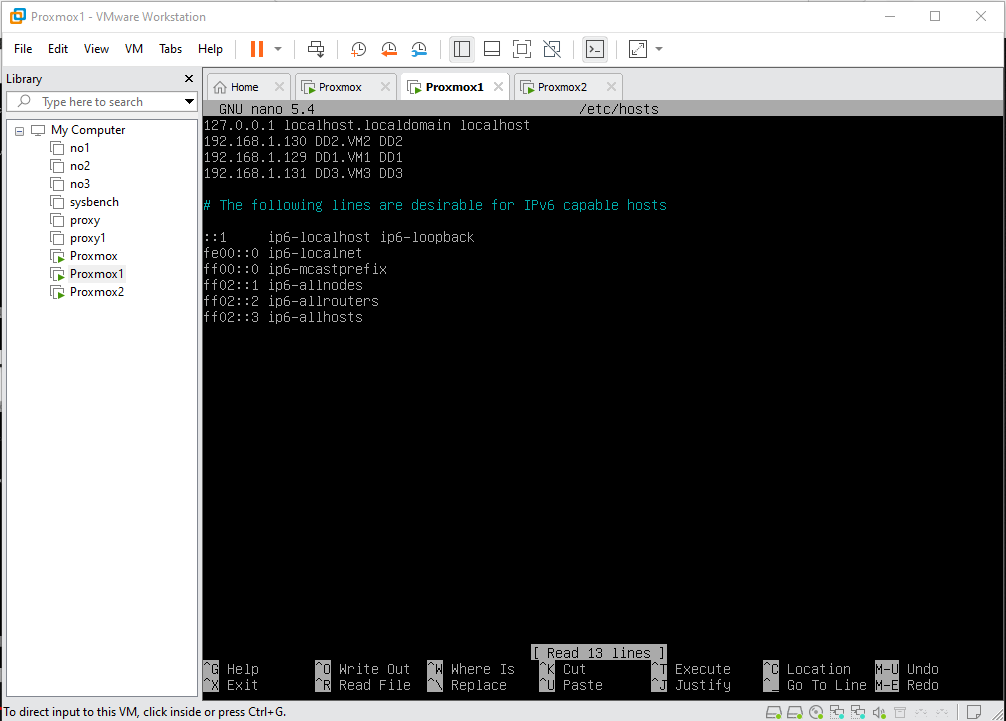
\includegraphics[width=14cm]{Screenshot_136.png}
\caption{Configuração do ficheiro Hosts no servidor 2}
\end{figure}

Servidor 3, Proxmox2 (DD3), foi adicionado o servidor 1 e 2.
\begin{verbatim}192.168.1.129 DD1.VM1 DD1\end{verbatim}
\begin{verbatim}192.168.1.130 DD2.VM2 DD2\end{verbatim}

\begin{figure}[H]
\center
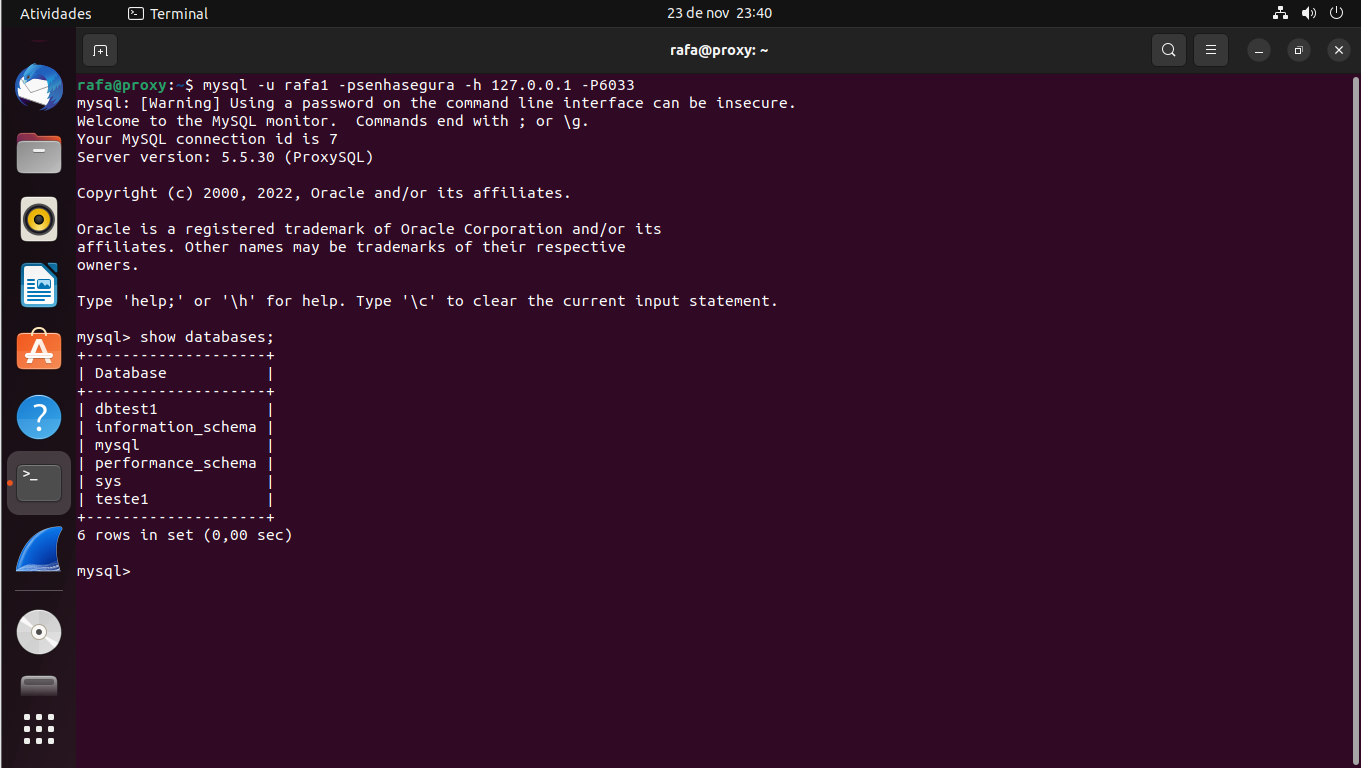
\includegraphics[width=13cm]{Screenshot_137.png}
\caption{Configuração do ficheiro Hosts no servidor 3}
\end{figure}


\section{Segunda Placa de Rede}
Adicionar uma segunda placa de rede a um sistema é uma maneira de criar redundância e garantir a disponibilidade da rede em caso de falha de uma das placas de rede. É especialmente útil em ambientes de alta disponibilidade \ac{HA}, onde é importante minimizar o tempo de inatividade (\textit{downtime}).

Para criar redundância com duas ou mais placas de rede, precisamos de configurar as placas de rede de forma a trabalharem em conjunto. Isso pode ser feito de várias maneiras, dependendo do \ac{SO} e do hardware utilizado. Algumas opções comuns são:

\begin{enumerate}
    \item Configurar as placas de rede para trabalhar em conjunto como um link ativo-passivo: uma placa de rede é configurada como principal e a outra é configurada como secundária. A placa principal é usada para o tráfego de rede, enquanto a placa secundária é usada apenas em caso de falha da placa principal.
    \item Configurar as placas de rede para trabalhar em conjunto como um link ativo-ativo: ambas as placas de rede são configuradas para trabalhar ao mesmo tempo e dividir o tráfego de rede. Isso pode ser feito usando técnicas como balanceamento de carga ou agregação de link.
    \item Configurar as placas de rede como um \textit{bond}: Um \textit{bond} é uma configuração de rede que permite combinar múltiplas placas de rede num único link. Isso permite criar uma conexão mais rápida e mais confiável, pois as placas de rede trabalham em conjunto para transmitir e receber dados.
\end{enumerate}

O meu objetivo com a segunda placa de rede foi criar boas práticas de implementação/configuração de rede apesar de no trabalho não aprofundar muito este tema (agregação de placas de rede) porque o principal foco não era este. Então, como acima mostrei (ambiente proxmox), tentei isolar a rede do cluster da rede de administração. Para isso criei uma segunda placa de rede para a rede do cluster (10.10.10.0).

\newpage
De seguida, mostro passo a passo da criação e configuração da segunda placa de rede.\\

Passo 1: Em \textbf{Virtual Machine Settings} do servidor proxmox, na aba de \textbf{Hardware} carregar em \textbf{Add...}.
\begin{figure}[H]
\center
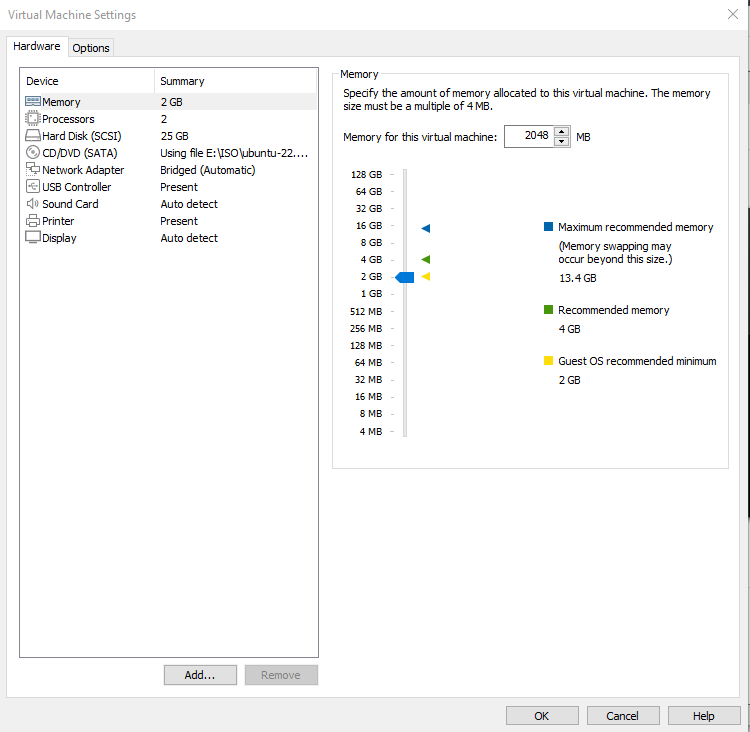
\includegraphics[width=14cm]{placa1.png}
\caption{Definições do servidor proxmox}
\end{figure}

\newpage
Passo 2: Como é uma placa de rede escolhemos \textbf{Network Adapter}.
\begin{figure}[H]
\center
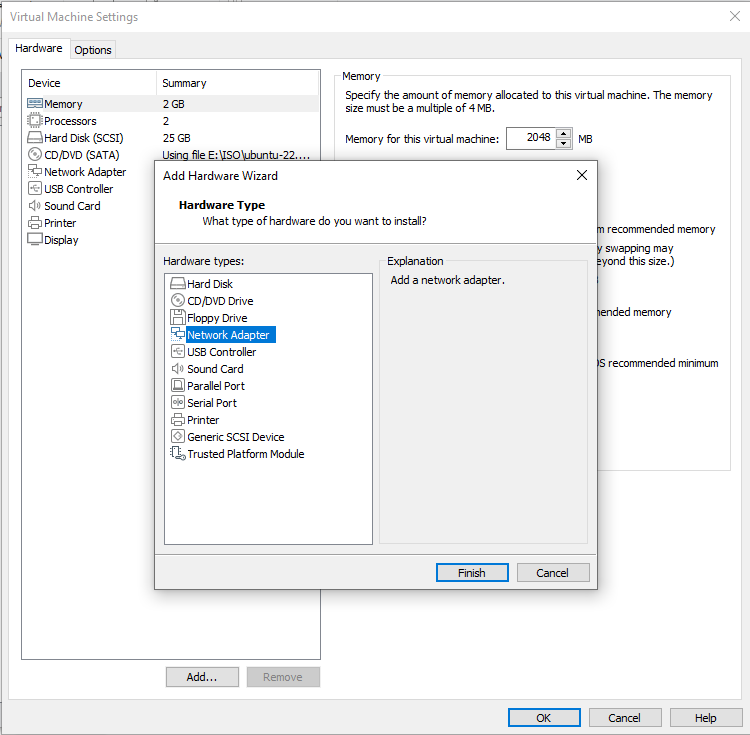
\includegraphics[width=14cm]{placa2.png}
\caption{Add Hardware Wizard}
\end{figure}

\newpage
Passo 3: Por fim, colocar a nova placa de rede (\textbf{Network Adpater 2}) em modo \textit{bridged}.
\begin{figure}[H]
\center
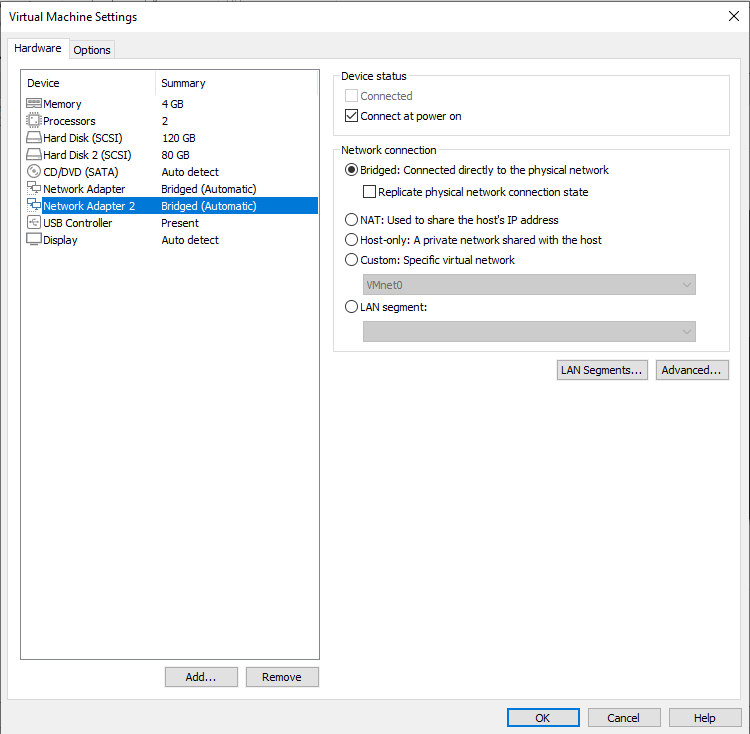
\includegraphics[width=14cm]{placa3.png}
\caption{Modo Bridge Placa de Rede}
\end{figure}

Para os outros 2 servidores é só repetir estes 3 passos anteriores.

\newpage
Passo 4: Depois de adicionar a nova placa de rede aos servidores e colocar em modo \textit{bridged}, na interface web dos 3 servidores proxmox já conseguimos ver a nova placa de rede (ens37). Para fazer a gestão da placas de rede no proxmox vamos ao nosso \textbf{Datacenter} e escolhemos o nosso servidor, no meu caso DD2, depois \textbf{System} e \textbf{Network}.
Por fim, foi só atribuir o \ac{IP} (10.10.10.130) à nova placa de rede carregando em \textbf{Edit}. Não esquecer de colocar a \textit{checkbox} \textbf{Autostart} marcada para a placa de rede iniciar sempre com o servidor.
\begin{figure}[H]
\center
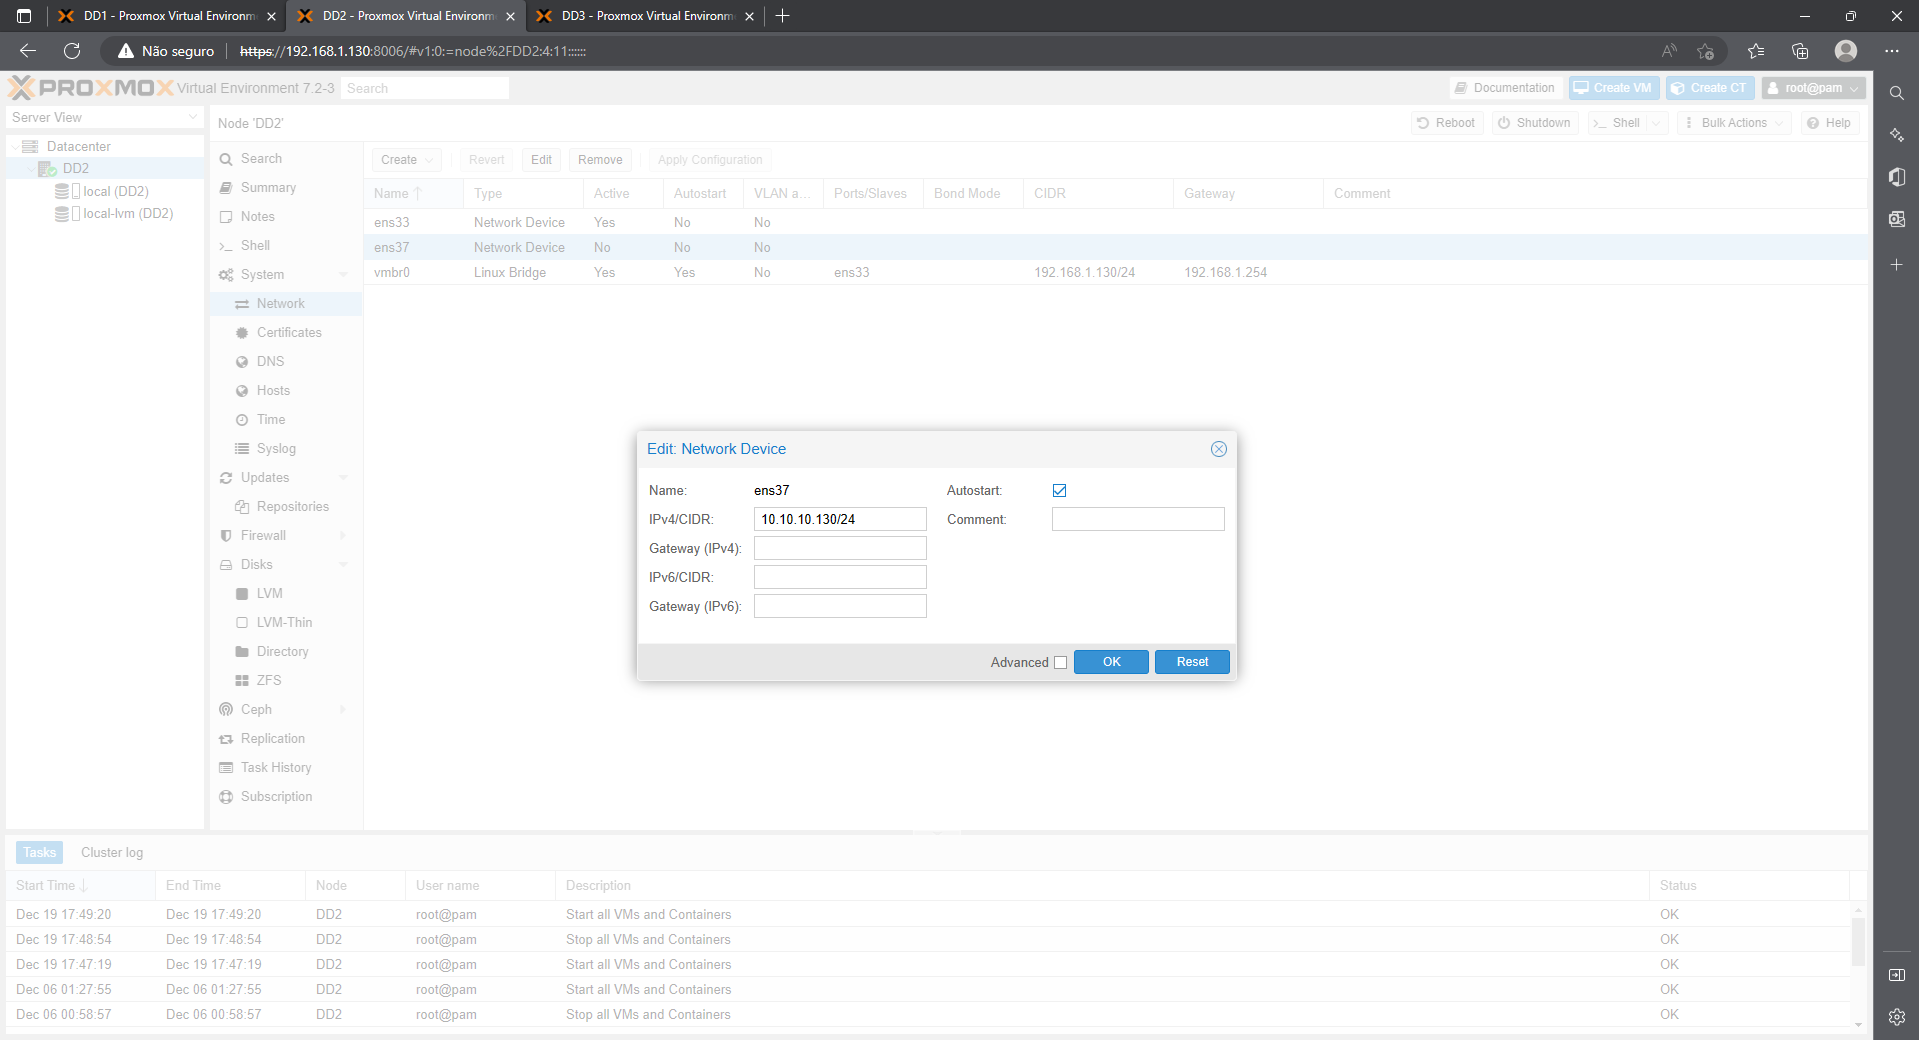
\includegraphics[width=14cm]{Screenshot_30.png}
\caption{\ac{IP} Segunda Placa de Rede}
\end{figure}

Passo 5: Depois de atribuir o \ac{IP} à placa de rede é sempre importante e necessário reiniciar o sistema.
\begin{figure}[H]
\center
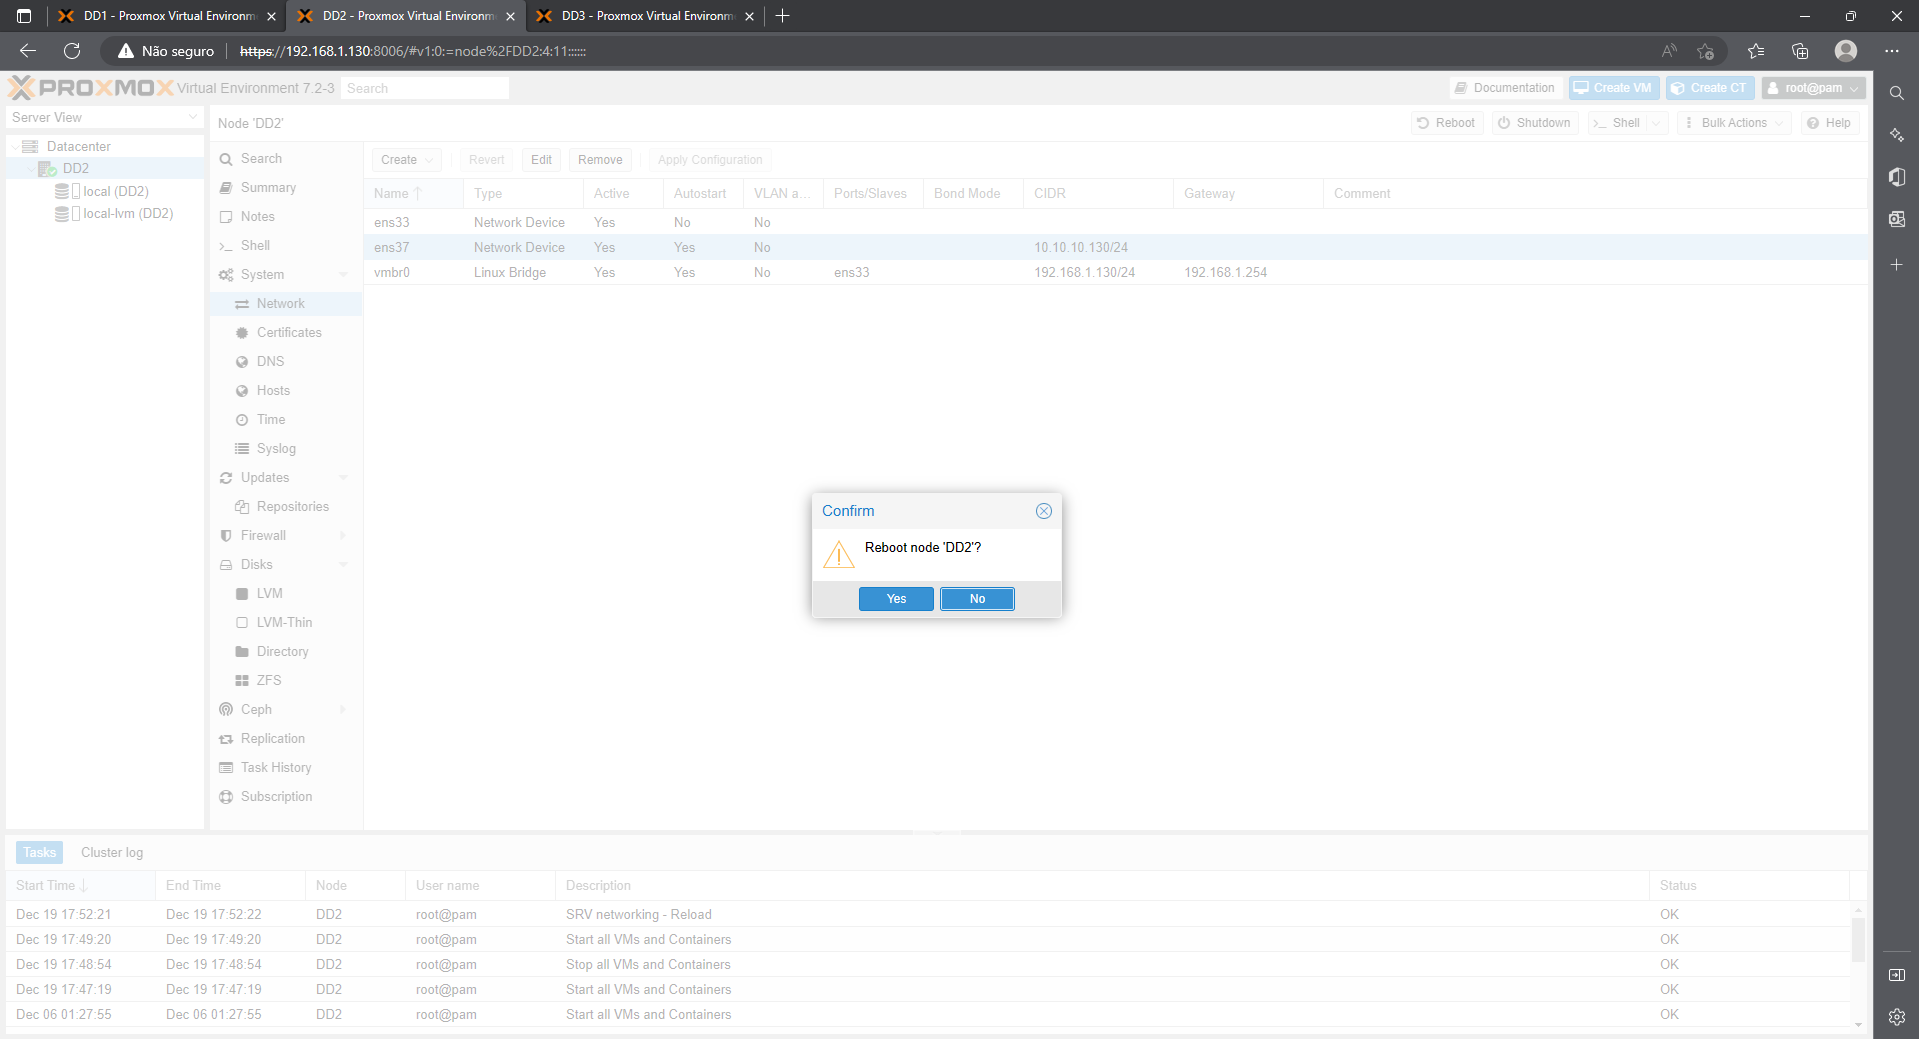
\includegraphics[width=14cm]{Screenshot_31.png}
\caption{Restart Node}
\end{figure}

Os passos anteriores são repetidos nos restantes servidores.

\newpage
Sem recorrer à interface gráfica do servidor também podemos configurar os passos anteriores através de linha de comandos, basta abrir a \textbf{shell} do servidor e temos acesso ao \ac{SO}. Como fiz a configuração na interface gráfica podemos verificar o ficheiro \textit{interfaces} do linux que contém a configuração das placas de rede. 
\begin{verbatim}nano /etc/network/interfaces\end{verbatim}

\begin{figure}[H]
\center
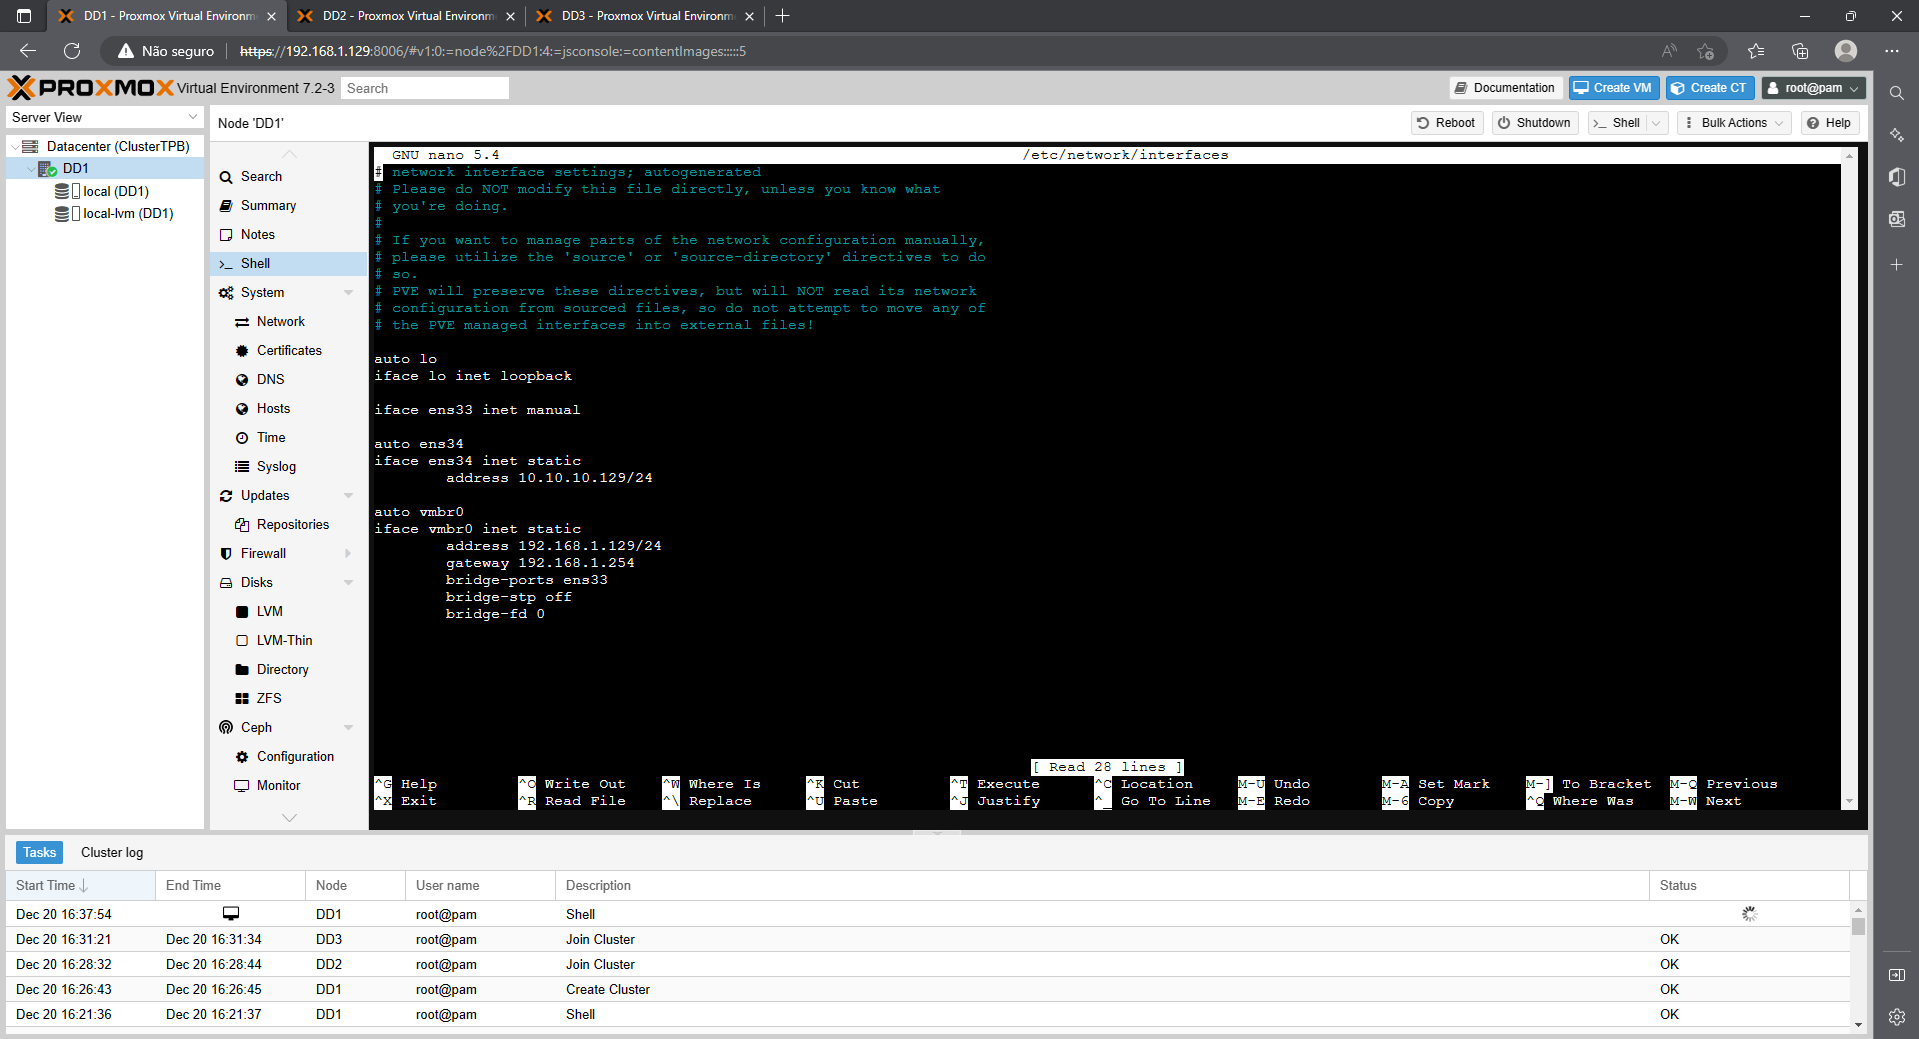
\includegraphics[width=14cm]{Screenshot_52.png}
\caption{Ficheiro configuração interfaces}
\end{figure}


\newpage
\section{Conectividade}
Feitas as instalações e configurações necessárias para obter um sistema funcional e comunicativo precisamos de verificar se os servidores conseguem comunicar entre si para poder avançar no projeto. Na \textbf{shell} de cada servidor foi feito um \textit{ping} para os restantes servidores para testar a conectividade.\\

DD1: Conseguiu "\textit{pingar}" o servidor DD2 e DD3 e ainda o exterior (1.1.1.1).
\begin{figure}[H]
\center
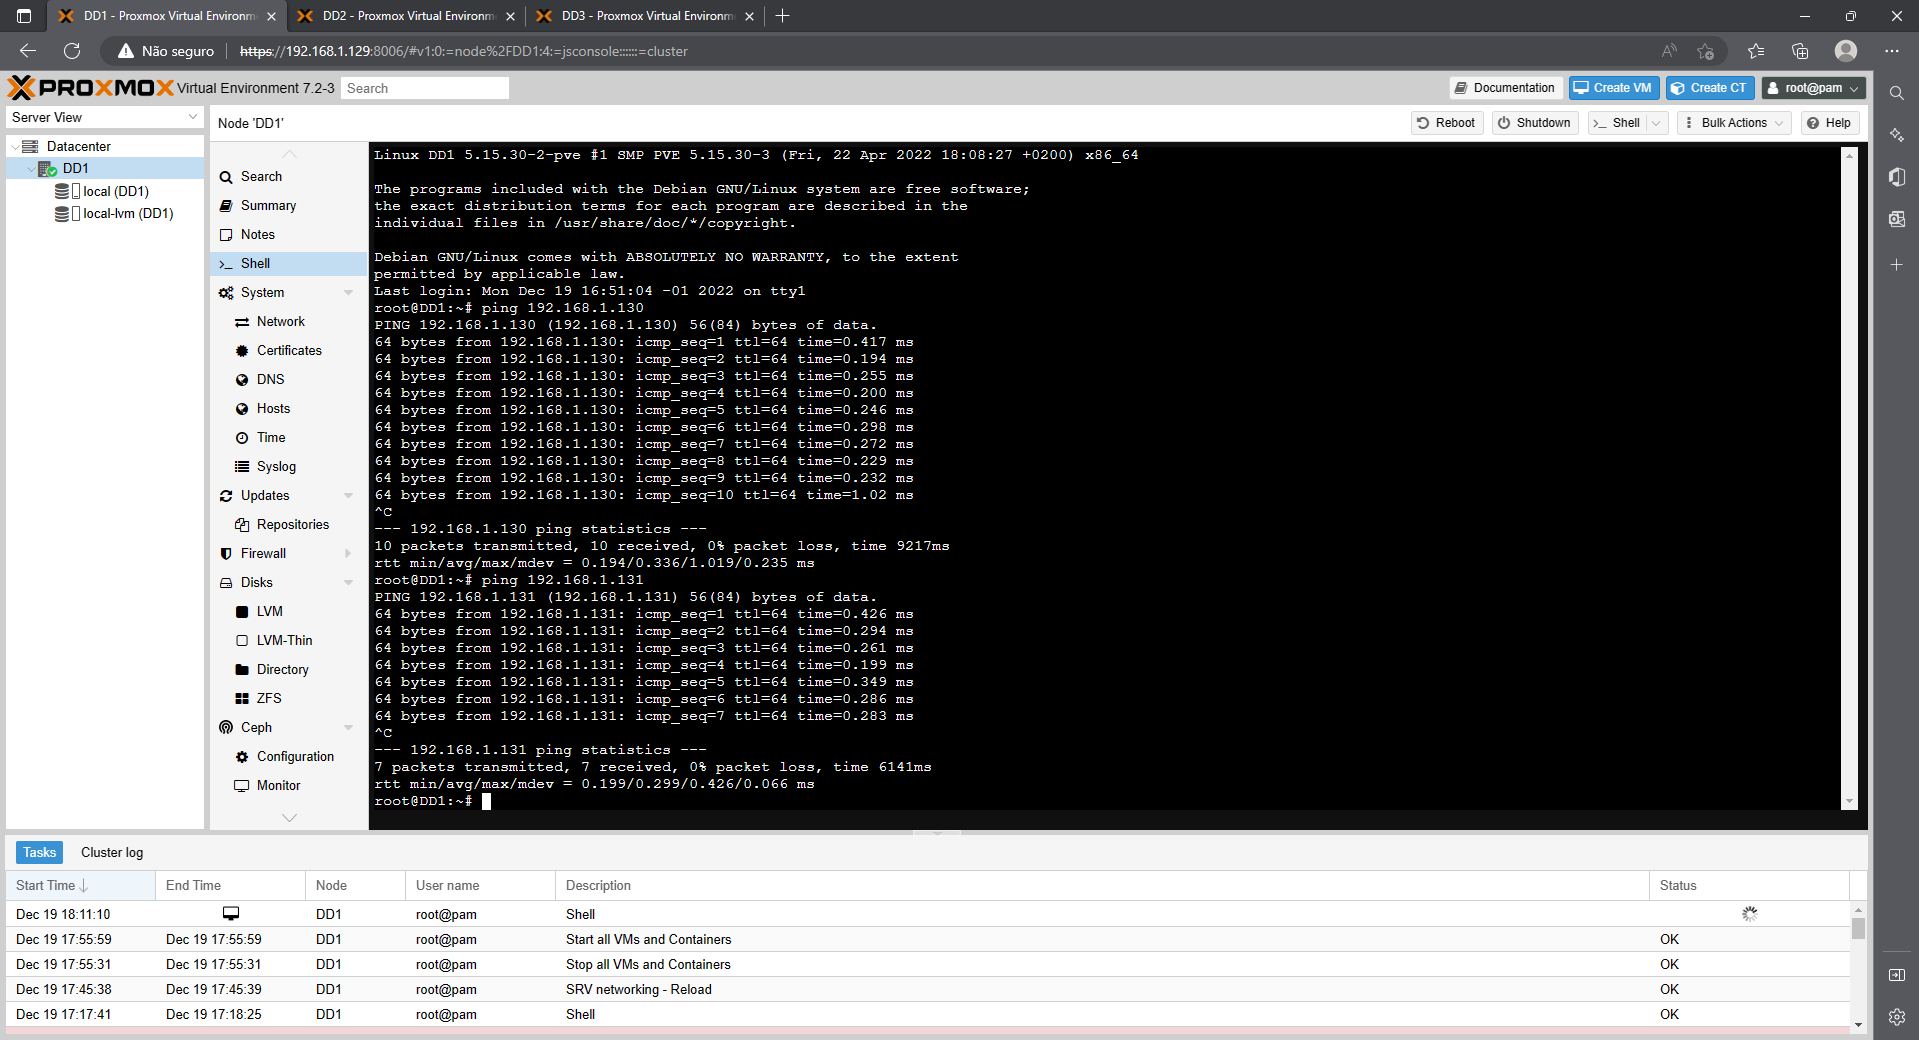
\includegraphics[width=14cm]{Screenshot_33.png}
\caption{Ping para DD2 e DD3}
\end{figure}

\begin{figure}[H]
\center
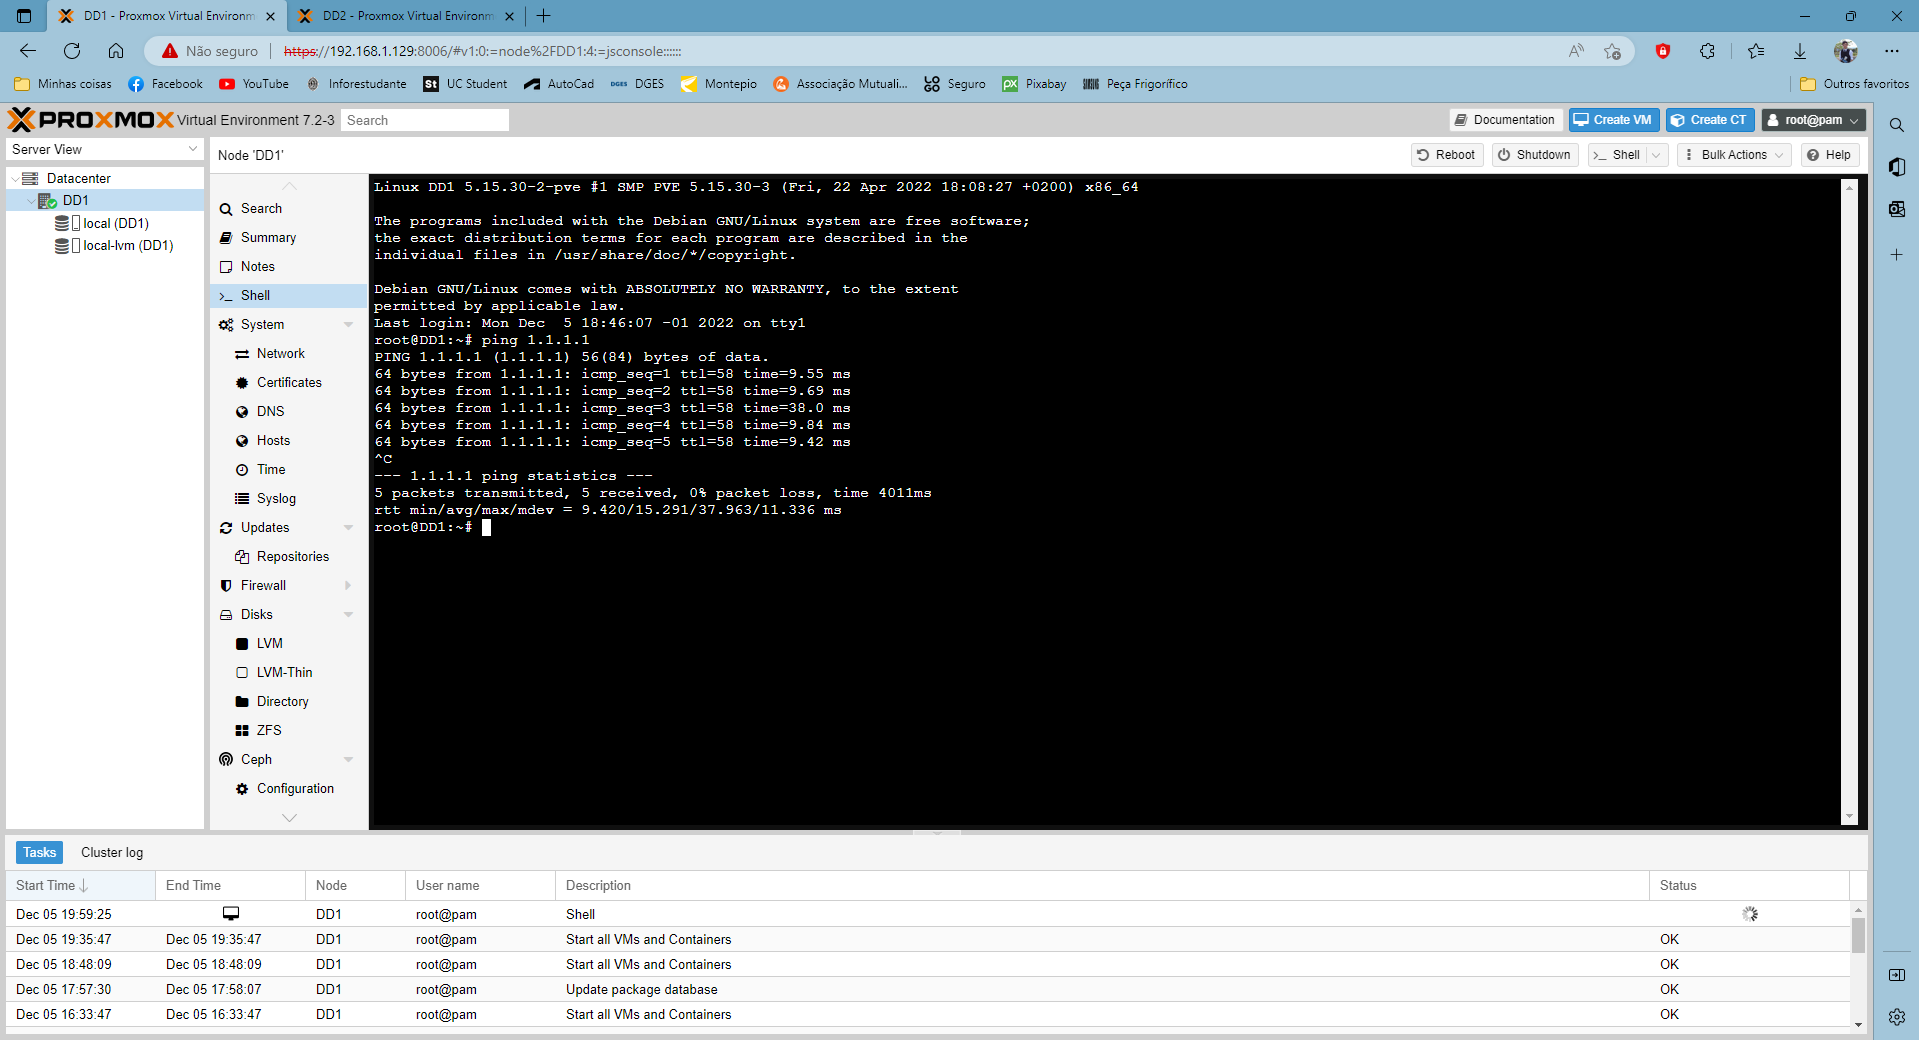
\includegraphics[width=14cm]{Screenshot_23.png}
\caption{Ping para o exterior}
\end{figure}

\newpage
DD2: Conseguiu "\textit{pingar}" o servidor DD1 e DD3.
\begin{figure}[H]
\center
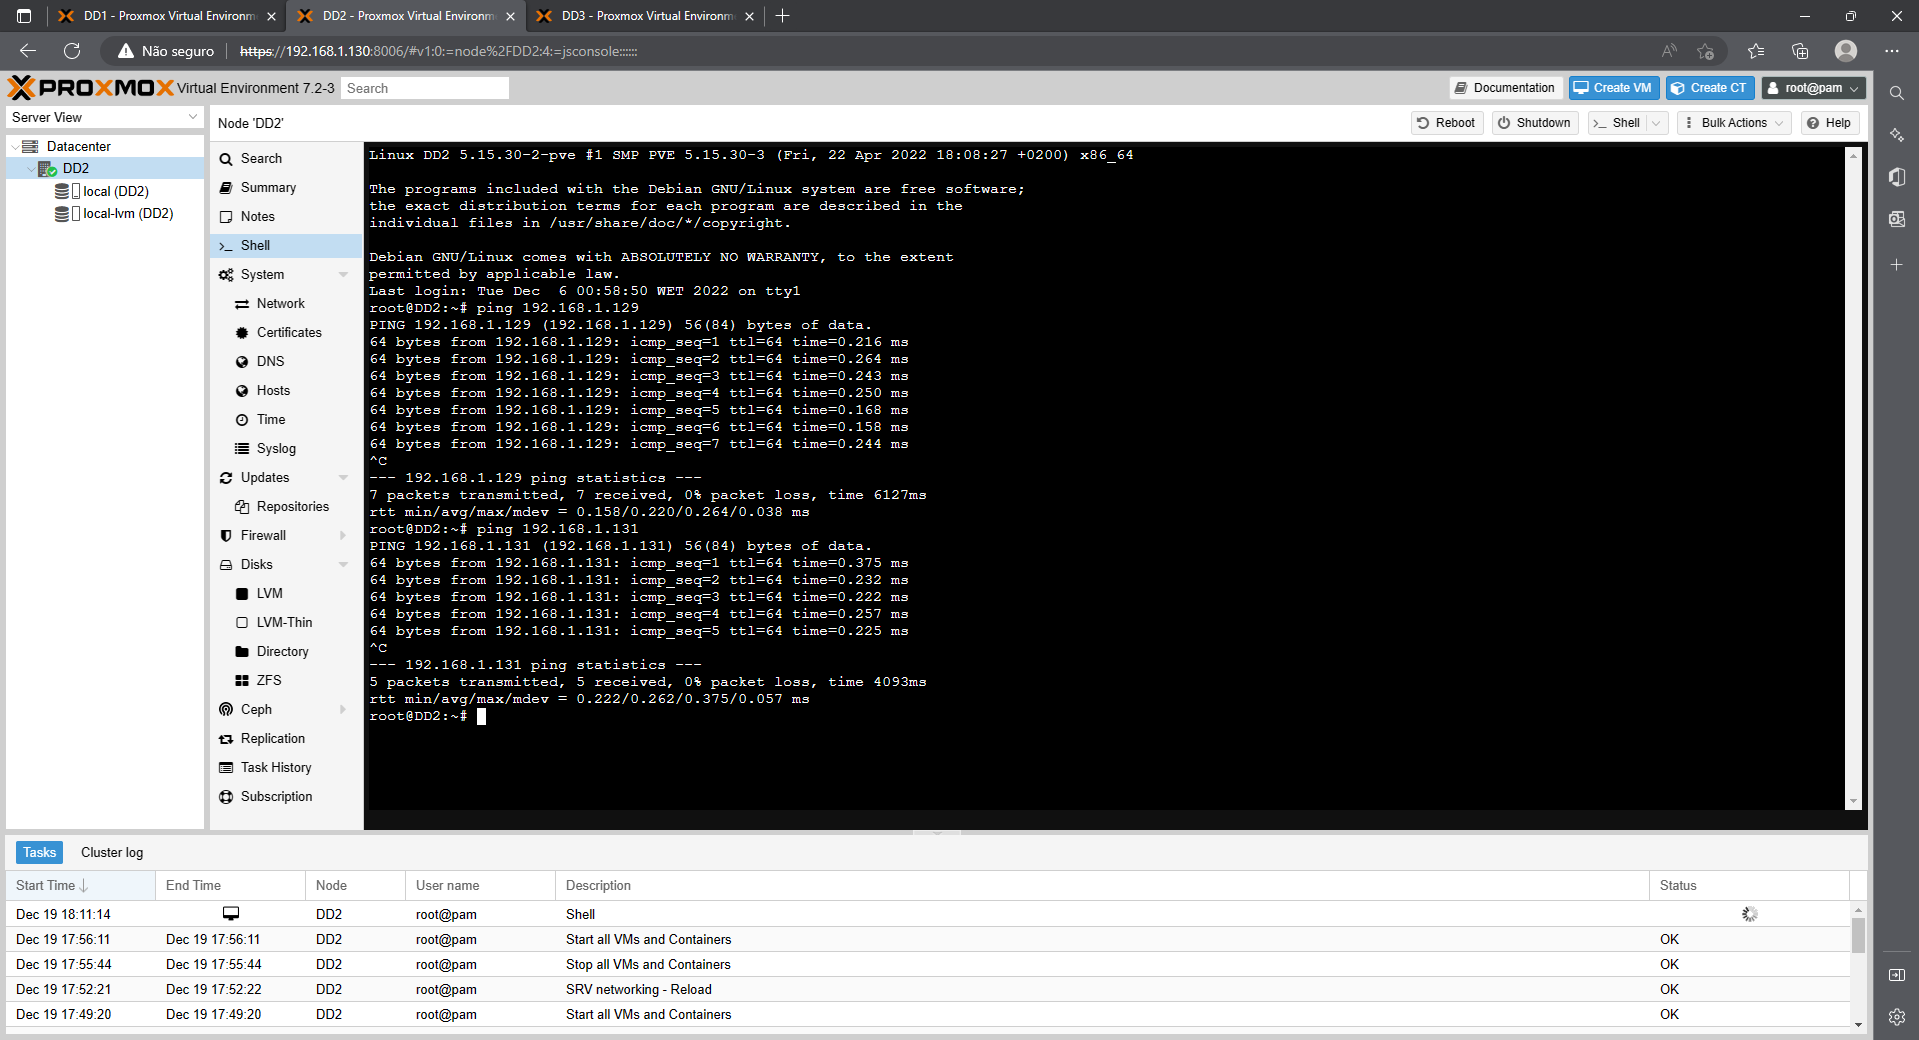
\includegraphics[width=14cm]{Screenshot_34.png}
\caption{Ping para DD1 e DD3}
\end{figure}

DD3: Conseguiu "\textit{pingar}" o servidor DD1 e DD2.
\begin{figure}[H]
\center
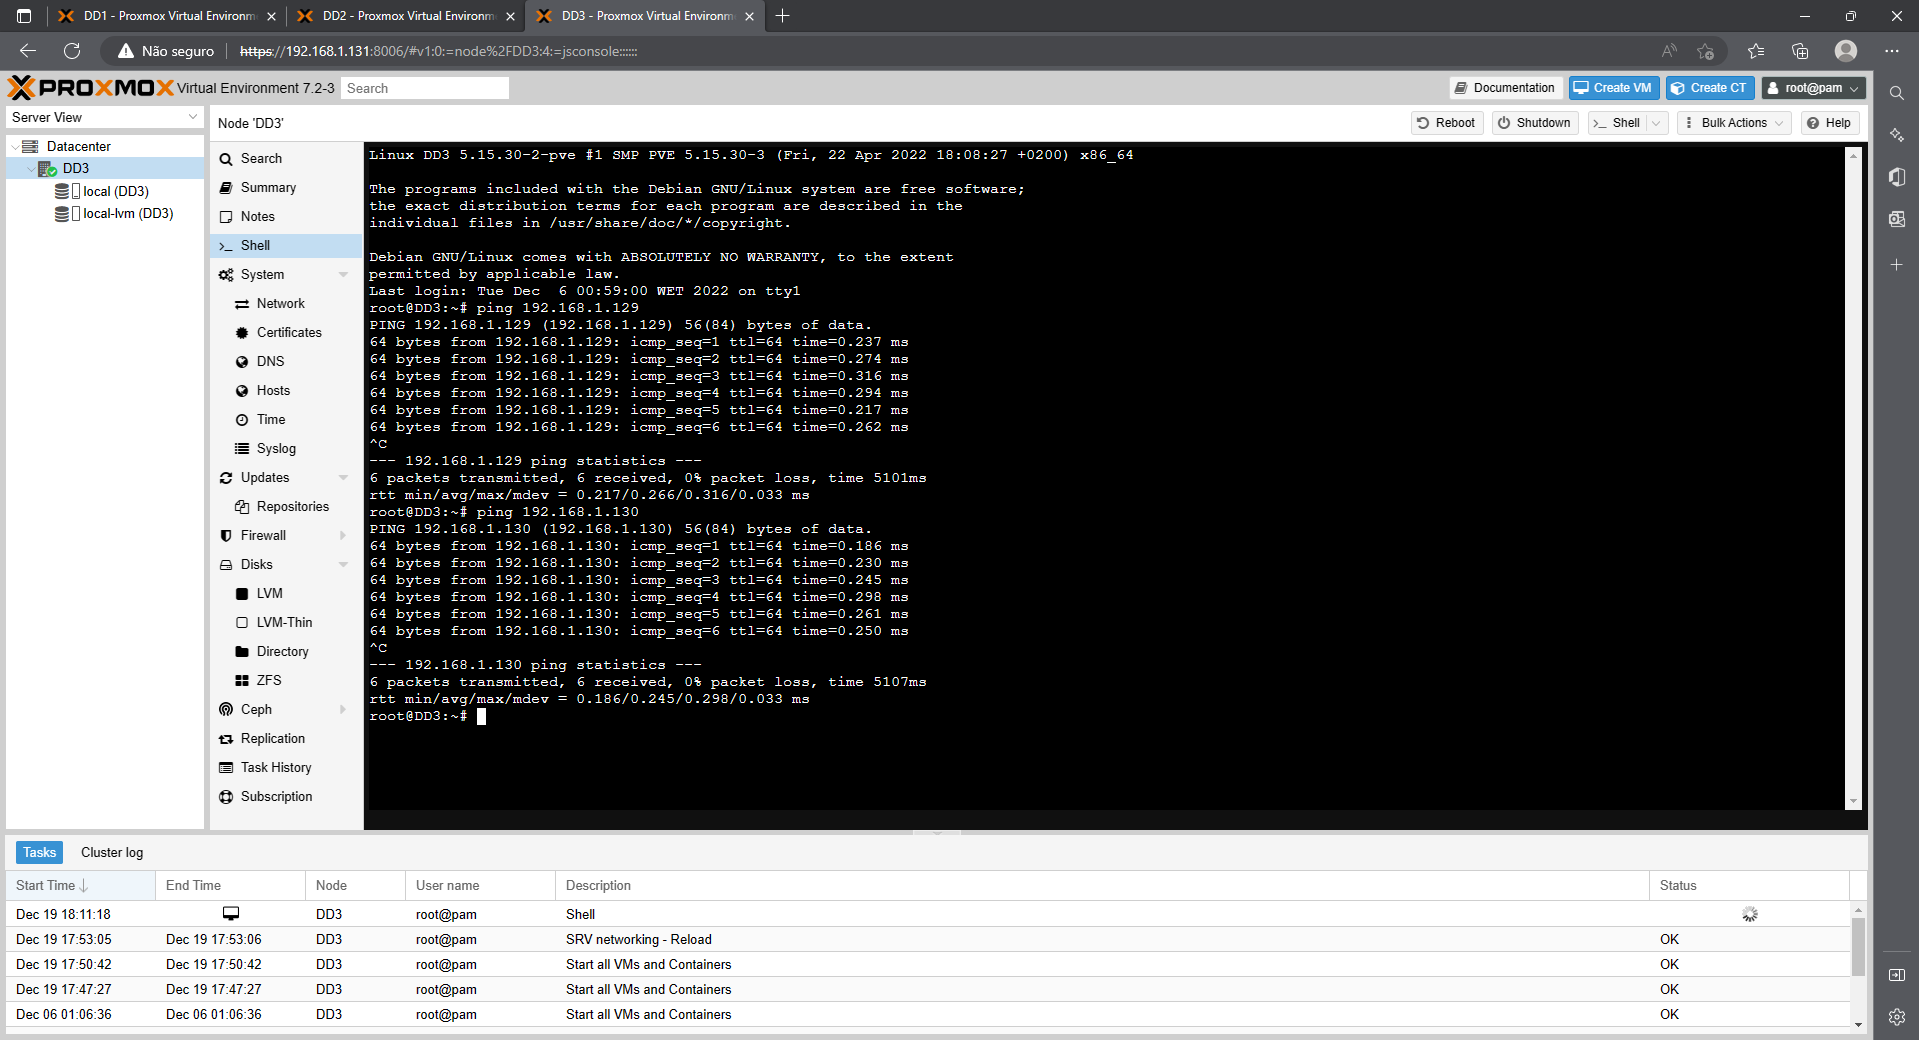
\includegraphics[width=14cm]{Screenshot_35.png}
\caption{Ping para DD1 e DD3}
\end{figure}

\newpage
Por fim, o DD1 ainda conseguiu "\textit{pingar}" a segunda interface de rede de DD2 (192.168.1.130).
\begin{figure}[H]
\center
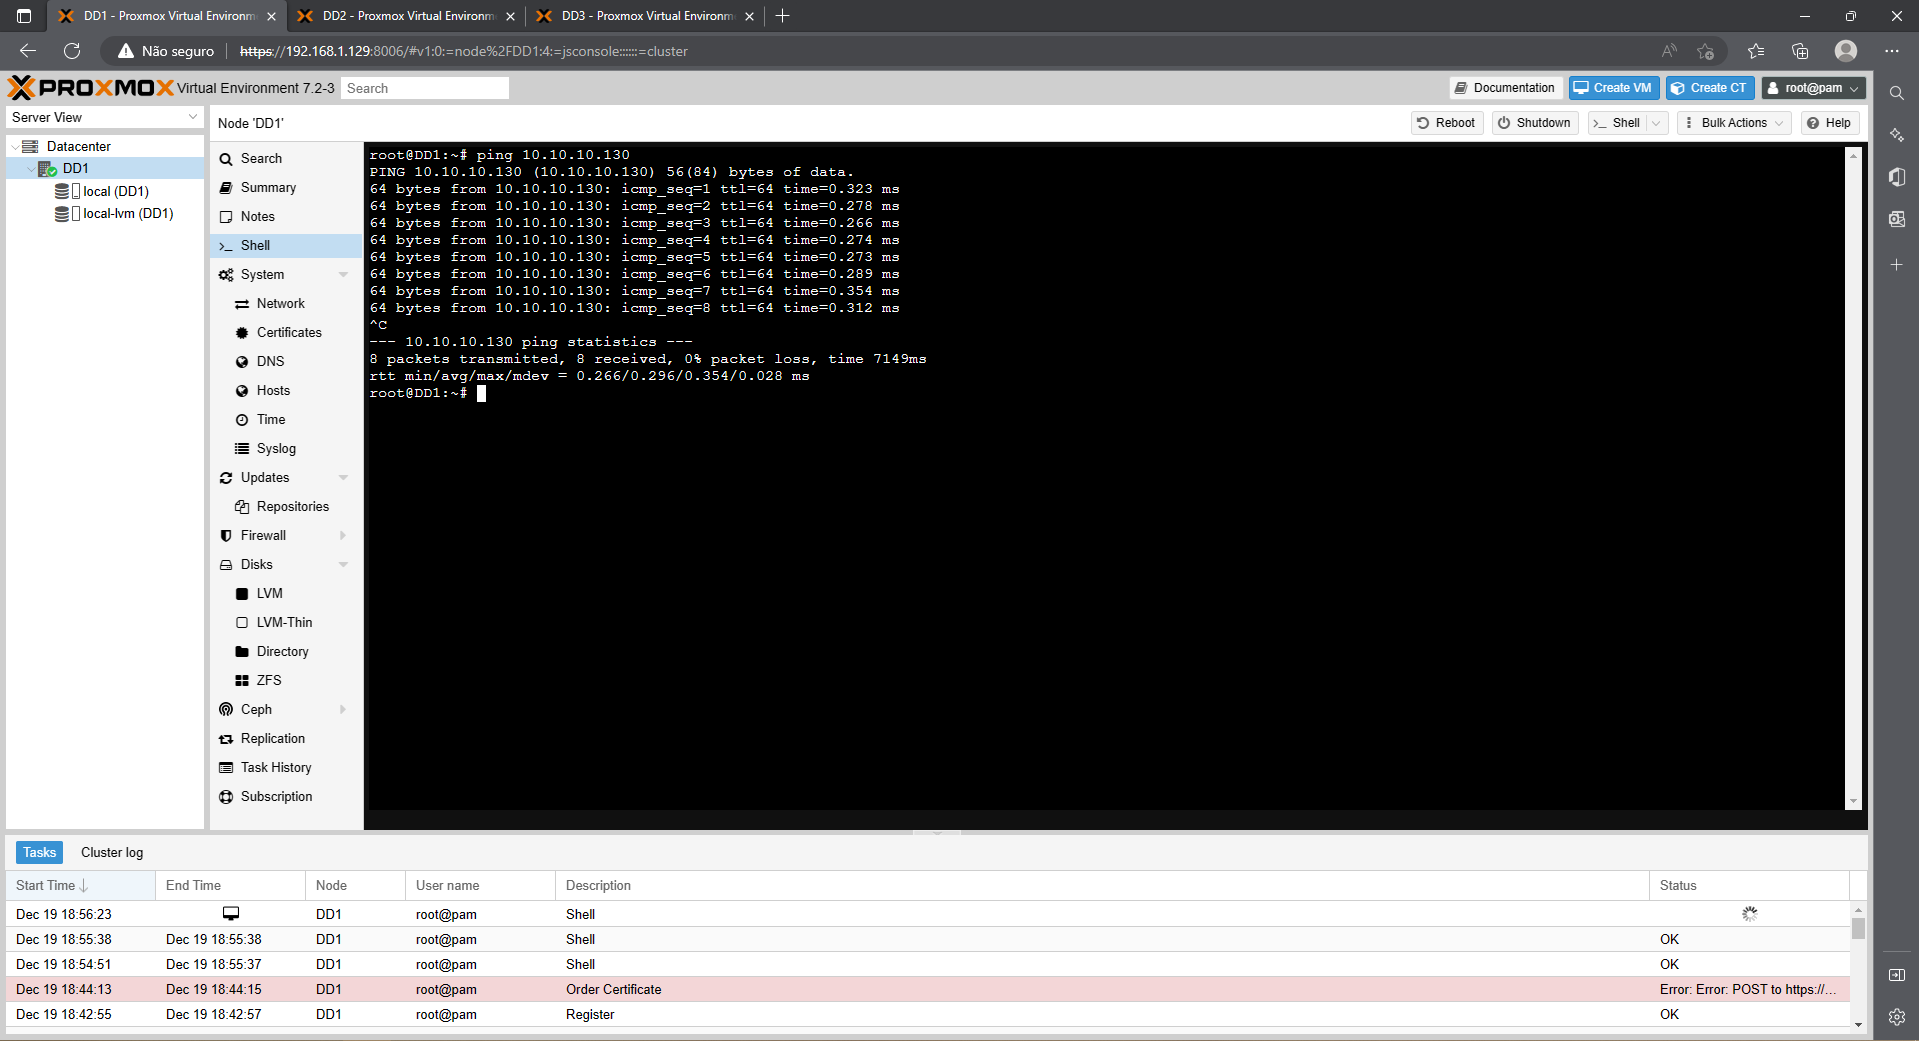
\includegraphics[width=14cm]{Screenshot_36.png}
\caption{Ping para segunda interface de rede DD2}
\end{figure}


Devido à configuração que foi feita inicialmente do ficheiro "hosts" também testei, no servidor DD2, "\textit{pingar}" por nome o servidor DD1.
\begin{figure}[H]
\center
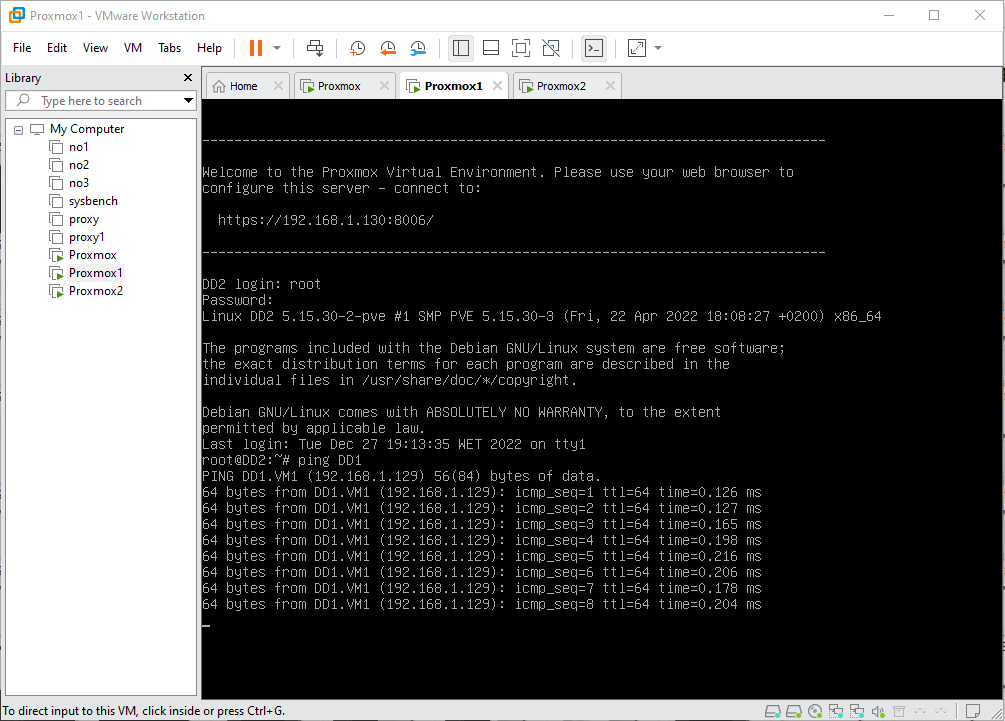
\includegraphics[width=14cm]{Screenshot_139.png}
\caption{Ping para segunda interface de rede DD2}
\end{figure}

\newpage
\section{Criação do Cluster}
O cluster, como já referido, é o funcionamento em conjunto de várias \ac{VM}. Para isso passamos à criação e configuração do cluster em proxmox.\\

Passo 1: Escolhi criar o cluster no servidor DD1 e os restantes apenas se conectavam ao cluster criado em DD1. O cluster é criado no \textbf{Datacenter}-\textbf{Cluster}-\textbf{Create Cluster}.
\begin{figure}[H]
\center
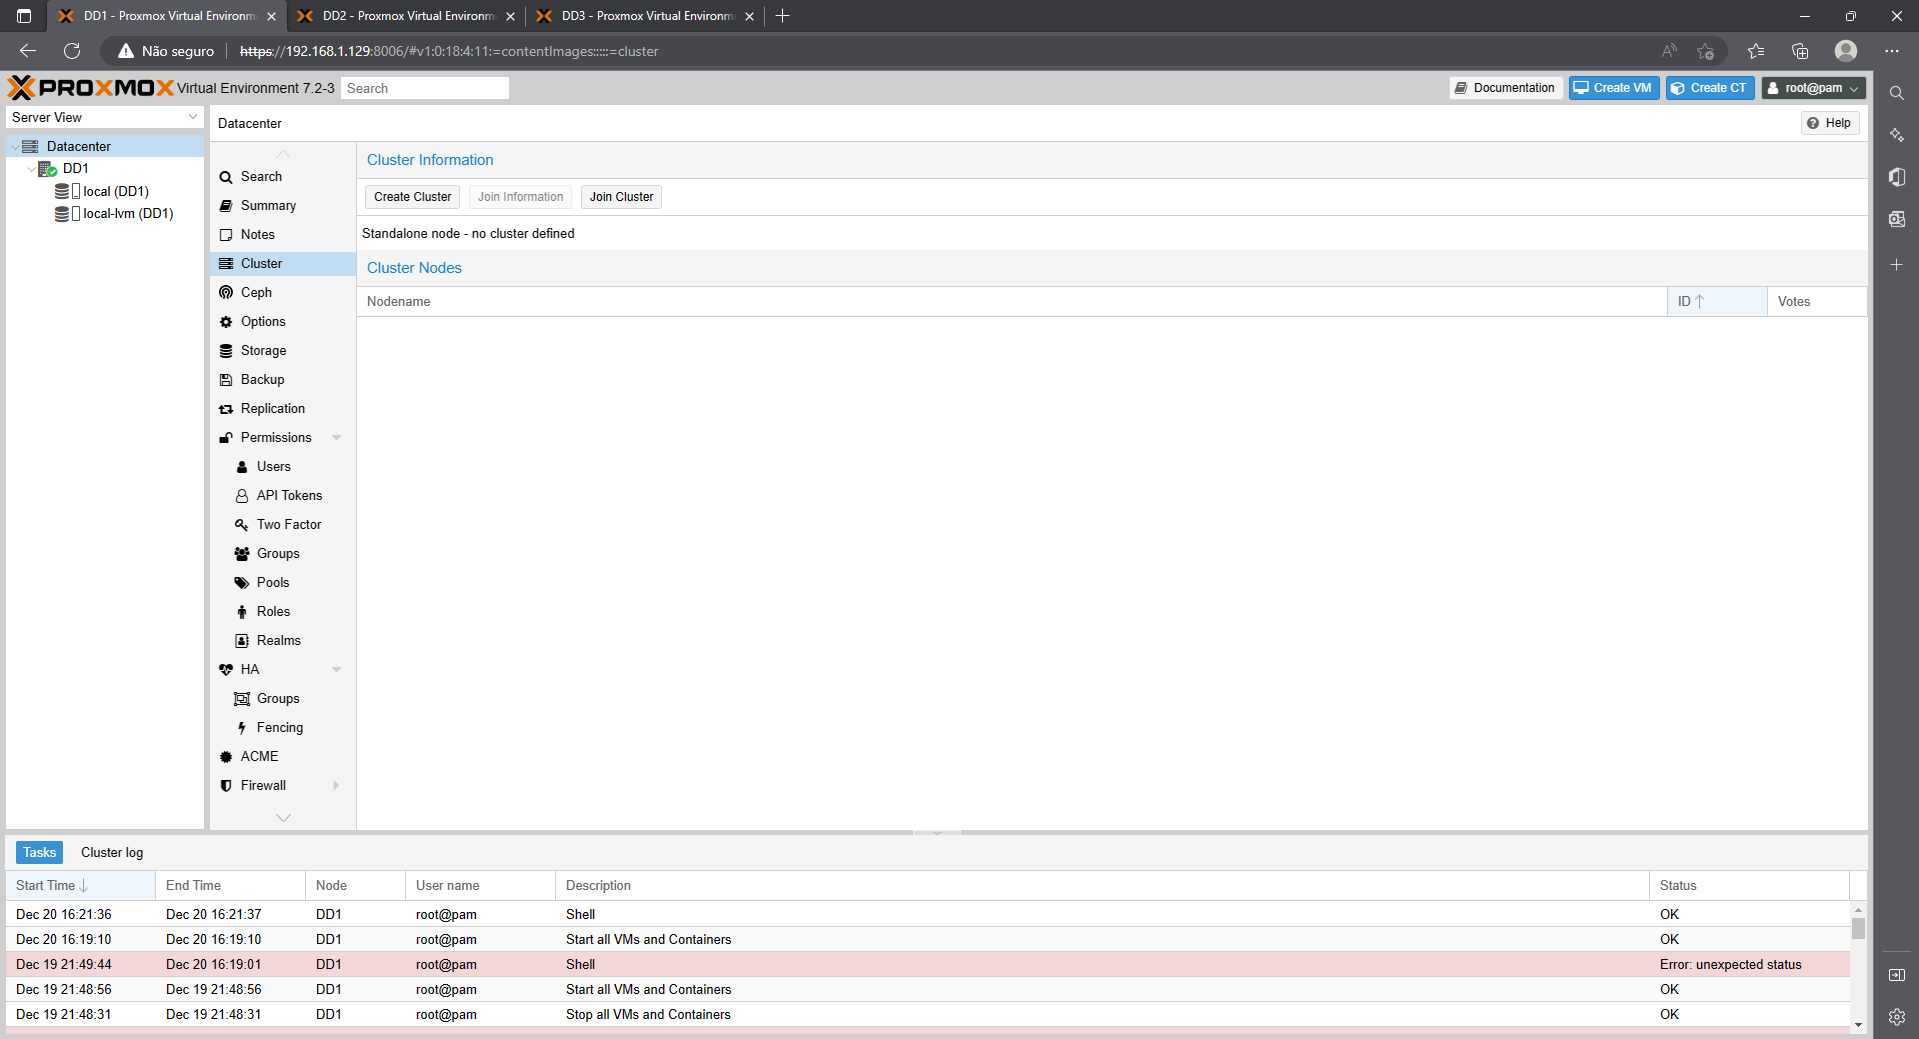
\includegraphics[width=14cm]{Screenshot_37.png}
\caption{Cluster}
\end{figure}

Passo 2: Nesta passo vamos atribuir um nome ao cluster, no meu caso chamei \textbf{clusterTPB,} e atribuir um ou mais \ac{IP} para criar redundância. Inseri apenas o \ac{IP} da rede do cluster (\textbf{10.10.10.129}).
\begin{figure}[H]
\center
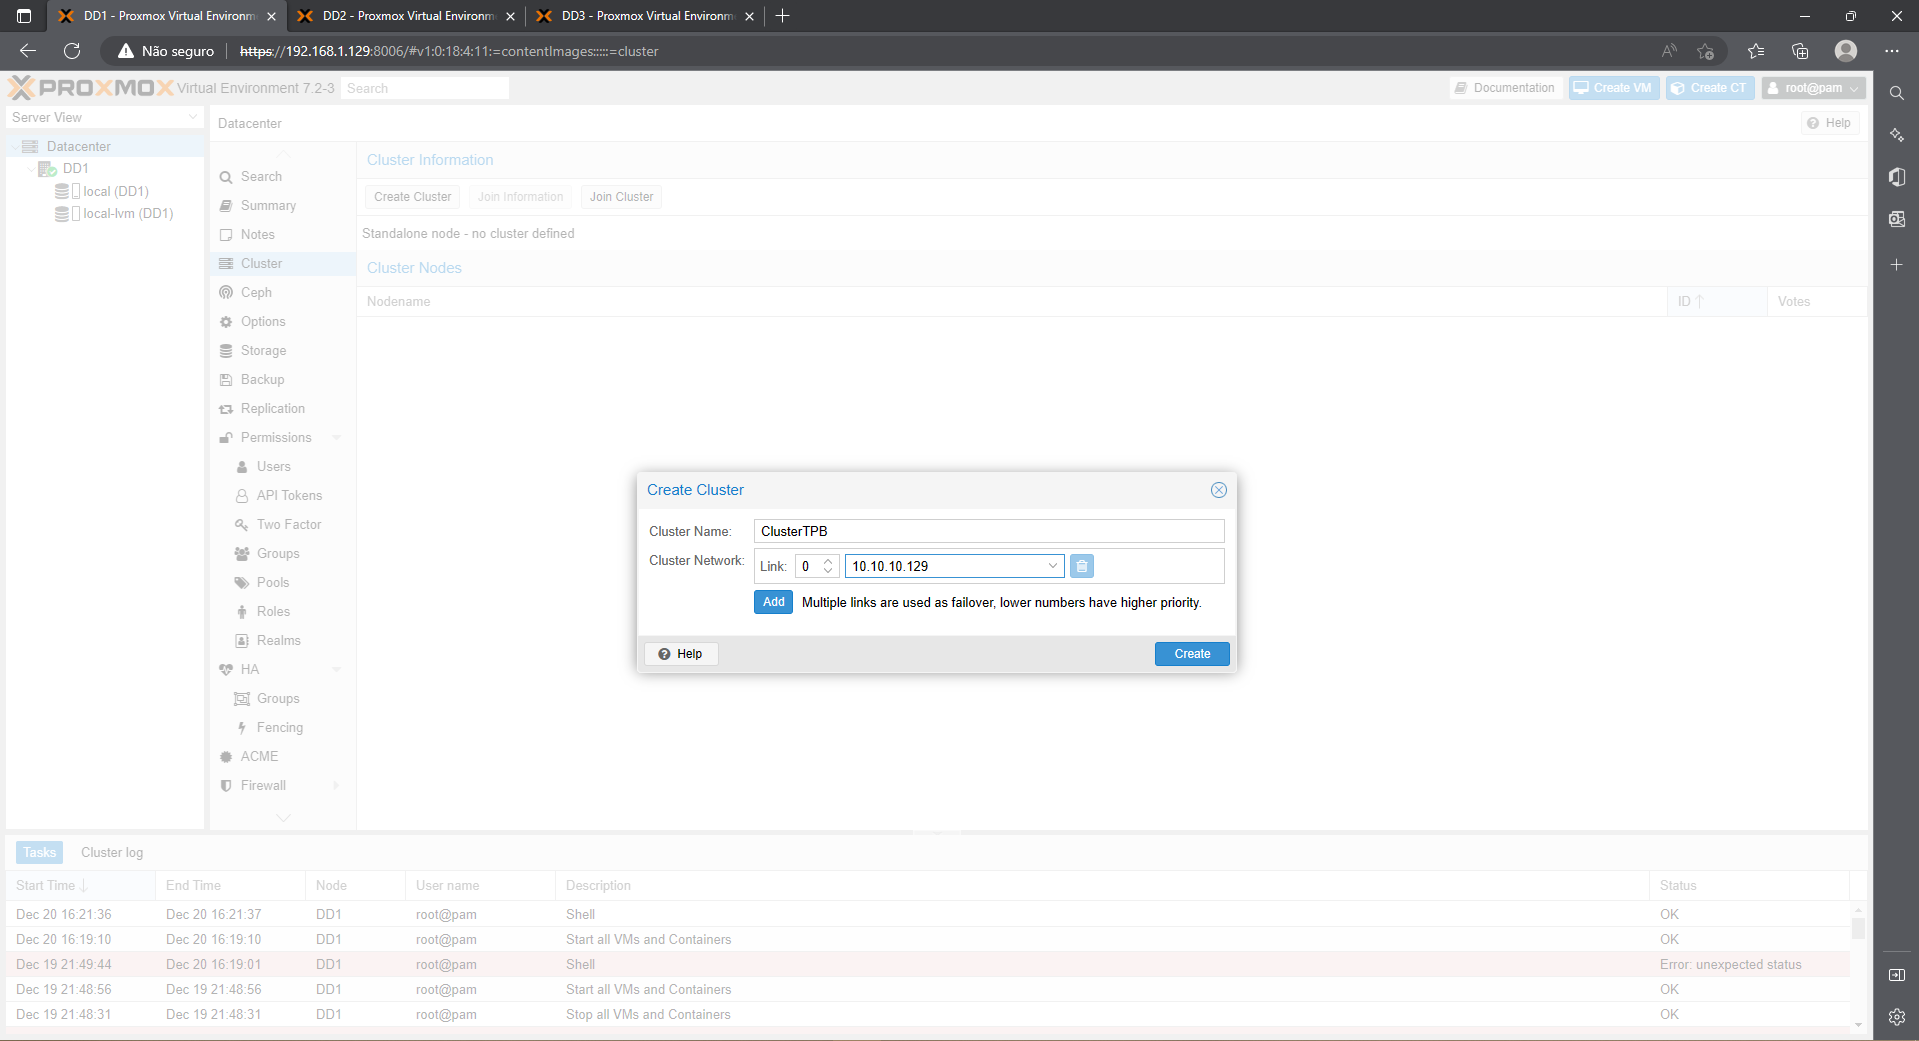
\includegraphics[width=14cm]{Screenshot_38.png}
\caption{Create Cluster}
\end{figure}

\newpage
De seguida podemos verificar alguns processos a serem iniciados, automaticamente, pelo proxmox, nomeadamente a configuração do \textit{corosync}. No final quando aparecer a informação de \textbf{TASK OK} podemos fechar a janela do \textit{Task Viewer} e o cluster está criado.
\begin{figure}[H]
\center
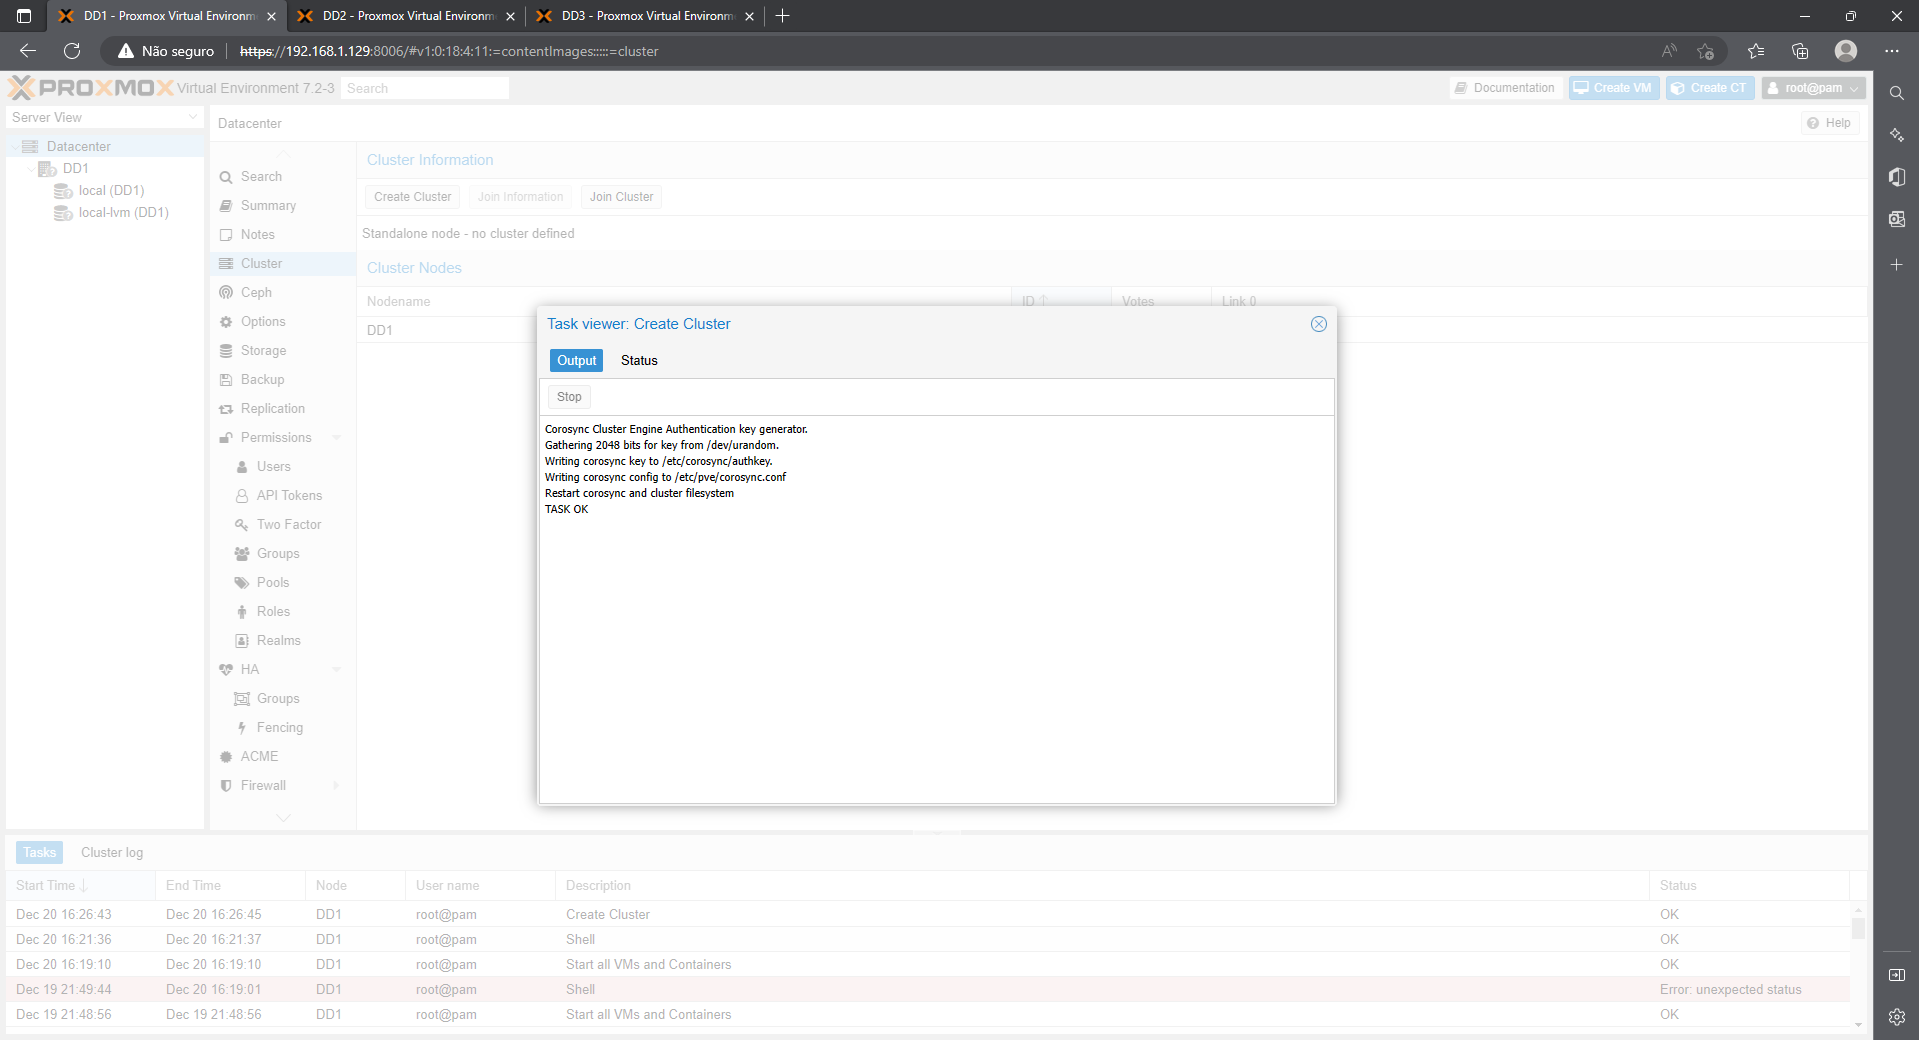
\includegraphics[width=14cm]{Screenshot_39.png}
\caption{Create Cluster Task Viewer}
\end{figure}

\begin{figure}[H]
\center
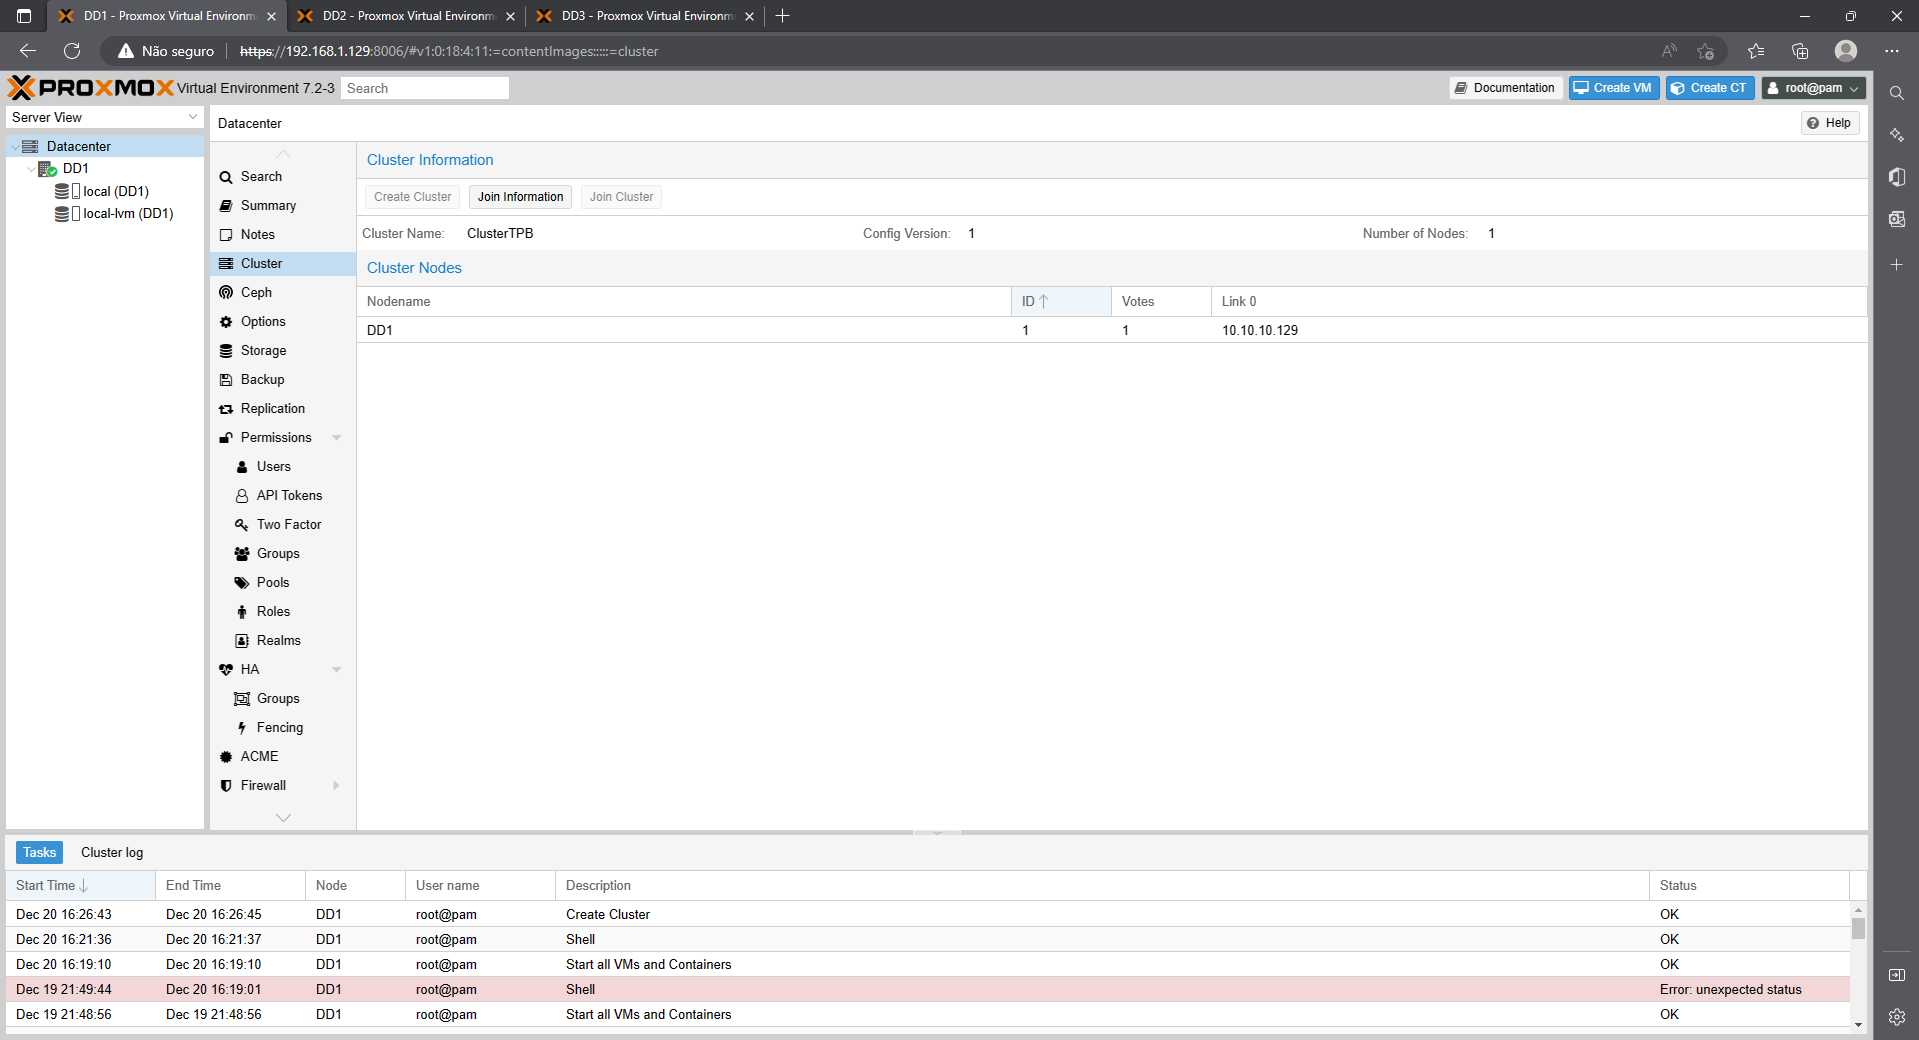
\includegraphics[width=14cm]{Screenshot_40.png}
\caption{Cluster Nodes DD1}
\end{figure}

\newpage
Um passo importante antes de adicionar os restantes nós ao cluster é copiar um conjunto de informações que se encontram em \textbf{Join Information} do nó criado (DD1). Apenas basta carregar em \textbf{Copy Information} e é selecionado e copiado automaticamente toda a informação.

\begin{figure}[H]
\center
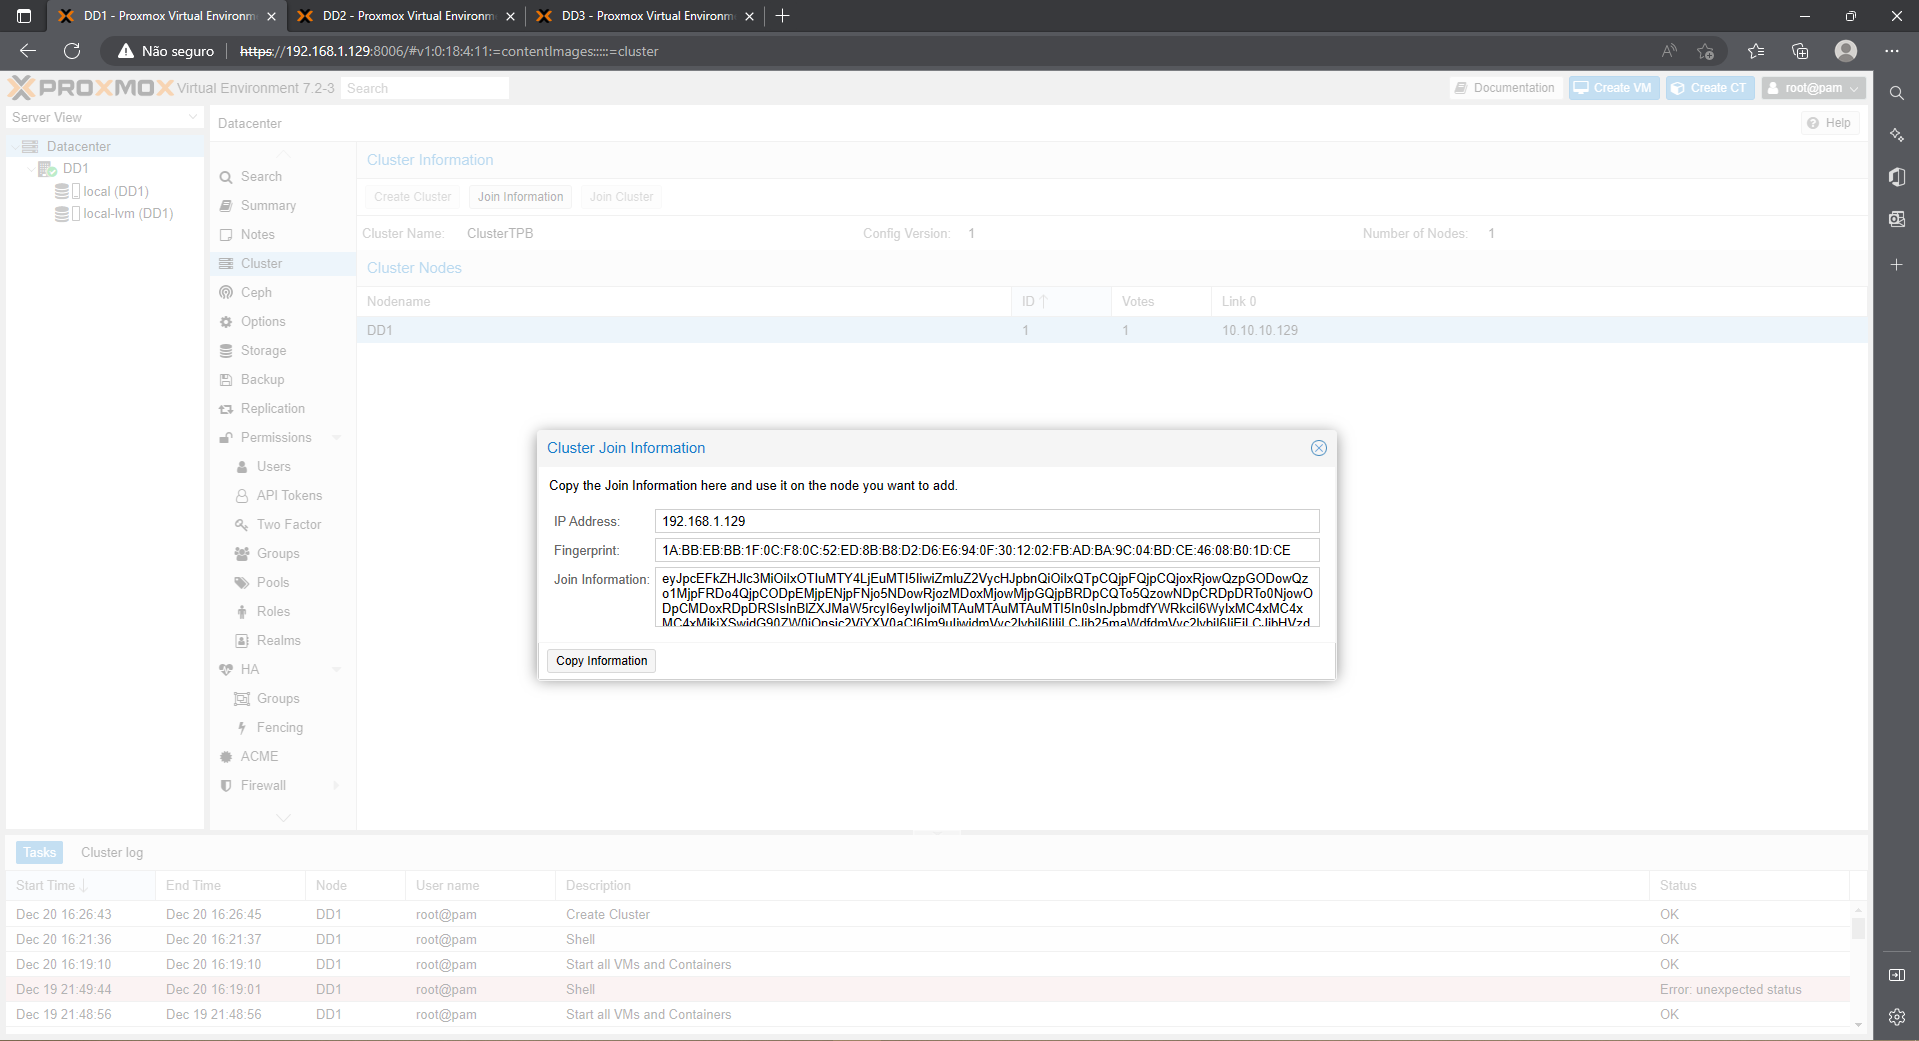
\includegraphics[width=14cm]{Screenshot_41.png}
\caption{Copy Information}
\end{figure}

Passo 3: No seguinte servidor, DD2, vamos novamente ao \textbf{Datacenter}-\textbf{Cluster} e agora não vamos criar um cluster porque já existe um. Vamos adicionar o nó DD2 ao cluster em DD1. Para isso precisamos de ir a \textbf{Join Cluster}.
\begin{figure}[H]
\center
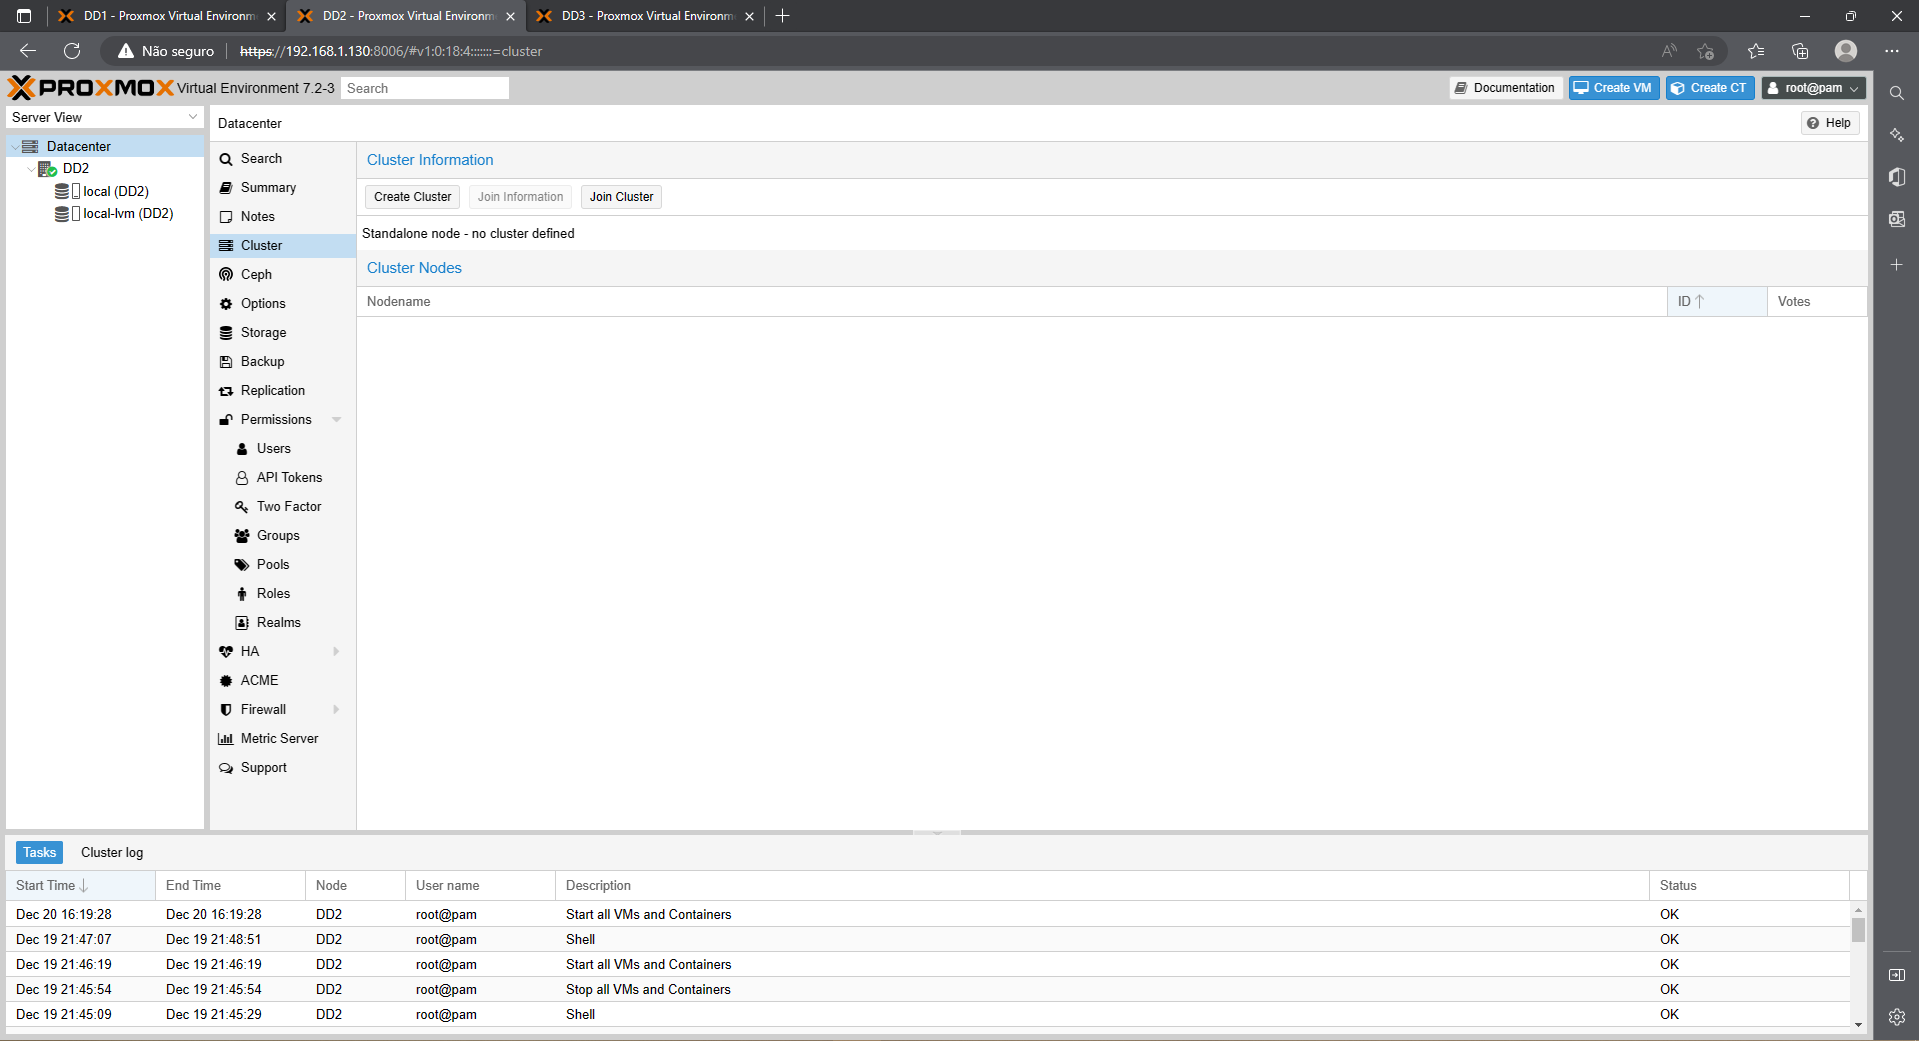
\includegraphics[width=14cm]{Screenshot_42.png}
\caption{Join Cluster}
\end{figure}

\newpage
Passo 4: No campo \textbf{Information} é onde vai ser colado a informação copiada do cluster em DD1. \textbf{Peer Address} é o \ac{IP} de administração do servidor DD1, 192.168.1.129. \textbf{Cluster Network} atribuiu o \ac{IP} da rede do cluster de DD2, 10.10.10.130. Por último inserir uma \textbf{Password}.
\begin{figure}[H]
\center
\includegraphics[width=14cm]{Screenshot_43.png}
\caption{Join Cluster}
\end{figure}

 No passo anterior depois de carregar em \textbf{Join ClusterTPB} podemos observar que no servidor DD2 já aparecem 2 nós, DD1 e DD2. Em DD1 também ja podems ver no \textbf{Datacenter} os nós do cluster.
\begin{figure}[H]
\center
\includegraphics[width=14cm]{Screenshot_44.png}
\caption{Cluster Nodes DD2}
\end{figure}

\begin{figure}[H]
\center
\includegraphics[width=14cm]{Screenshot_45.png}
\caption{Cluster Nodes DD1}
\end{figure}

Para o cluster ficar completo, no servidor DD3 repetimos o passo 3 e 4 e obtemos o cluster com os 3 nós.

\begin{figure}[H]
\center
\includegraphics[width=14cm]{Screenshot_46.png}
\caption{Cluster DD3}
\end{figure}

\begin{figure}[H]
\center
\includegraphics[width=14cm]{Screenshot_47.png}
\caption{Cluster Join}
\end{figure}

\begin{figure}[H]
\center
\includegraphics[width=14cm]{Screenshot_48.png}
\caption{Cluster Nodes DD3}
\end{figure}

\newpage
Em DD1 também já podemos ver o cluster completo.
\begin{figure}[H]
\center
\includegraphics[width=14cm]{Screenshot_49.png}
\caption{Cluster DD1}
\end{figure}

A partir de agora pode-se trabalhar apenas numa interface web de um servidor à escolha, eu usei sempre o DD1, 192.168.1.129. Como o cluster já esta completo a replicação já está a funcionar entre os nós, por isso o que for feito num nó será replicado entre os restantes.\\

Por fim, podemos observar a configuração do ficheiro \textit{corosync}:

\begin{figure}[H]
\center
\includegraphics[width=14cm]{Screenshot_180.png}
\caption{Configuração Corosync}
\end{figure}

\begin{figure}[H]
\center
\includegraphics[width=14cm]{Screenshot_181.png}
\caption{Configuração Corosync}
\end{figure}

Para observar algumas informações acerca do cluster, nodes, resources do Datacenter entre outros, podemos observar em \textbf{Datacenter}-\textbf{Summary}.
\begin{figure}[H]
\center
\includegraphics[width=14cm]{Screenshot_50.png}
\caption{Datacenter Summary}
\end{figure}


\newpage
\section{Ceph}

Para criar o sistema de armazenamento distribuído passamos para a instalação e configuração do \textit{Ceph}.\\

Passo 1: Instalação do \textit{Ceph} em cada "nó".
\begin{figure}[H]
\center
\includegraphics[width=14cm]{Screenshot_51.png}
\caption{Instalação Ceph}
\end{figure}

Passo 2: A versão escolhida foi 16.2 (pacific). Existiam outras.
\begin{figure}[H]
\center
\includegraphics[width=14cm]{Screenshot_53.png}
\caption{Versão do Ceph}
\end{figure}

\newpage
Passo 3: Durante o processo de instalação vai ser preciso confirmar a continuação.
\begin{figure}[H]
\center
\includegraphics[width=14cm]{Screenshot_54.png}
\caption{Continuação da instalação}
\end{figure}

Passo 4: Configuração do \textit{Ceph}.
Em \textbf{Public Network} fica a rede que foi criada para separar o \textit{Cluster} da rede de "Administração": \textbf{10.10.10.129/24} e \textbf{Cluster Network} a rede da "Administração": \textbf{192.168.1.129/24}.
Para terminar, no Monitor a escolha é \textbf{DD1}.
\begin{figure}[H]
\center
\includegraphics[width=14cm]{Screenshot_56.png}
\caption{Configuração do \textit{Ceph}}
\end{figure}

\newpage
Por último, a instalação e configuração fica finalizada.
\begin{figure}[H]
\center
\includegraphics[width=14cm]{Screenshot_57.png}
\caption{Término da instalação}
\end{figure}

Podemos verificar que no "nó" DD1 foi criado o \textit{Monitor}.
\begin{figure}[H]
\center
\includegraphics[width=14cm]{Screenshot_60.png}
\caption{Monitor DD1}
\end{figure}

\newpage
Nos restantes "nós" temos de repetir os passos anteriores para cada um deles ficar com o \textit{Ceph}.
Existe uma diferença na configuração e que não foi preciso configurar porque automaticamente é preenchida.
\begin{figure}[H]
\center
\includegraphics[width=14cm]{Screenshot_59.png}
\caption{Configuração nos restantes nós}
\end{figure}

No "nó" DD2 podemos verificar que já existem os dois \textit{Monitor}.
\begin{figure}[H]
\center
\includegraphics[width=14cm]{Screenshot_62.png}
\caption{Monitor DD2}
\end{figure}

\newpage
Caso algum monitor não seja criado automaticamente com a instalação do \textit{Ceph}, é preciso adicionar manualmente. Para isso precisamos de ir a: \textbf{Ceph}-\textbf{Monitor}-\textbf{Create}. No meu caso foi o DD3.
\begin{figure}[H]
\center
\includegraphics[width=14cm]{Screenshot_64.png}
\caption{Create Monitor DD3 Manualmente}
\end{figure}

Por último, podemos veirifcar que todos os "nós" possuem os vários \textit{Monitor}.
\begin{figure}[H]
\center
\includegraphics[width=14cm]{Screenshot_65.png}
\caption{Monitor do Cluster}
\end{figure}

\newpage
Podemos verificar o estado (\textit{Health}) do \textit{Ceph}. Neste momento vai indicar um \textit{WARNING} porque ainda não existem \ac{OSD} criados.
\begin{figure}[H]
\center
\includegraphics[width=14cm]{Screenshot_66.png}
\caption{Configuração do \textit{Ceph}}
\end{figure}

\subsection{OSD}
Cada \ac{OSD} faz a gestão de armazenamento de cada "nó" e para isso foi preciso criar de seguida um novo "disco" para associar a cada \ac{OSD}. Disco esse que vai ser replicado pelo \textit{Cluster}.

Passo 1: Adicionar mais um \textit{Hard Disk} a cada servidor no \textit{VMWare}.
\begin{figure}[H]
\center
\includegraphics[width=14cm]{Screenshot_69.png}
\caption{Adicionar Hard Disk}
\end{figure}

\newpage
Passo 2: Escolha do tipo de Disco: \textbf{\ac{SCSI}}.
\begin{figure}[H]
\center
\includegraphics[width=14cm]{Screenshot_70.png}
\caption{Escolha de Tipo de Disco}
\end{figure}

Passo 3: Por defeito escolhi \textbf{Create a new virtual disk}.
\begin{figure}[H]
\center
\includegraphics[width=14cm]{Screenshot_71.png}
\caption{Create New vitual Disk}
\end{figure}

\newpage
Passo 4: Capacidade do disco: 80Gb.
\begin{figure}[H]
\center
\includegraphics[width=14cm]{Screenshot_72.png}
\caption{Capacidade do disco}
\end{figure}

Passo 5: Por defeito optei por deixar o nome do ficheiro \textit{vmdk} e finalizar.
\begin{figure}[H]
\center
\includegraphics[width=14cm]{Screenshot_73.png}
\caption{Término da criação do novo disco}
\end{figure}

Nos restantes servidores é só repetir os passos anteriores para adicionar um novo disco ao servidor.

\newpage
Passo 6: Depois de adicionar um novo disco aos servidores, criei então o \ac{OSD} com o devido disco.
\begin{figure}[H]
\center
\includegraphics[width=14cm]{Screenshot_67.png}
\caption{Create OSD}
\end{figure}

\begin{figure}[H]
\center
\includegraphics[width=14cm]{Screenshot_74.png}
\caption{Escolha do disco}
\end{figure}

\newpage
Em DD1 e DD2 já podemos verificar o \ac{OSD} criado com o disco de 80Gb agregado.
\begin{figure}[H]
\center
\includegraphics[width=14cm]{Screenshot_75.png}
\caption{OSD DD1}
\end{figure}

\begin{figure}[H]
\center
\includegraphics[width=14cm]{Screenshot_76.png}
\caption{OSD DD2}
\end{figure}

\newpage
Para obter todos os \ac{OSD} no \textit{Cluster} apenas foi preciso repetir o passo 6.
No final podemos observar que em DD1 e nos restantes "nós" existem os três \ac{OSD}.

\begin{figure}[H]
\center
\includegraphics[width=14cm]{Screenshot_78.png}
\caption{OSD Cluster}
\end{figure}

Depois de ter adicionado um novo disco aos servidores e ter criado os \ac{OSD} podemos confirmar que o \textit{Ceph} está com boa "saúde". 
\begin{figure}[H]
\center
\includegraphics[width=14cm]{Screenshot_79.png}
\caption{Health Ceph}
\end{figure}

\newpage
\subsection{Pools}
\textit{Pools} são partições lógicas usadas para armazenar objetos. Objetos esses que ficam armazenados no núcleo do \textit{Ceph}, \ac{RADOS}. Para criar a \textit{pool} de armazenamento apenas é preciso criar uma vez. Neste caso criei em DD1.\\

Passo 1: Em \textbf{DD1}-\textbf{Ceph}-\textbf{Pools}-\textbf{Create}, criei a \textit{pool} indicando apenas um nome.
\begin{figure}[H]
\center
\includegraphics[width=14cm]{Screenshot_81.png}
\caption{Pool Create}
\end{figure}

Como no \textit{Cluster} existem menos de 5 OSD, os \ac{PG} ficam definidos com o número de 128.\\

Depois de ter criado a \textit{pool} de armazenamento podemos verificar que foi criada e replicada no \textit{cluster}.
\begin{figure}[H]
\center
\includegraphics[width=14cm]{Screenshot_82.png}
\caption{Pool Create}
\end{figure}

\newpage
De seguida, ao verificar a \textit{Health} do \textit{Ceph} podemos observar os \ac{PG} a 33.
\begin{figure}[H]
\center
\includegraphics[width=14cm]{Screenshot_84.png}
\caption{Health Ceph}
\end{figure}

\newpage
\section{Criação Máquina Virtual}
Para testar a migração precisamos de criar uma máquina virtual/container. De seguida segue o registo do passo a passo da criação da máquina virtual.\\

Passo 1: \textit{Upload} do ficheiro \textit{ISO}. Neste caso foi usado o Ubuntu Server 22.04.
\begin{figure}[H]
\center
\includegraphics[width=14cm]{Screenshot_110.png}
\caption{Upload ISO}
\end{figure}

Depois da importação finalizada é esperado o "\textbf{TASK OK}".
\begin{figure}[H]
\center
\includegraphics[width=14cm]{Screenshot_111.png}
\caption{Task Ok Upload}
\end{figure}

\newpage
Passo 2: Depois de ter o ficheiro \textit{ISO} no servidor podemos criar a máquina virtual. \textbf{DD1}-\textbf{Create VM}.Em General:\\
\textbf{Node}: "nó" onde colocar a \ac{VM};\\
\textbf{VM ID}: um ID para a \ac{VM};\\
\textbf{Name}: Nome da \ac{VM}.
\begin{figure}[H]
\center
\includegraphics[width=14cm]{Screenshot_112.png}
\caption{Create Virtual Machine-General}
\end{figure}

Passo 3: Em OS:\\
\textbf{Storage}: local;\\
\textbf{ISO image}: escolher o ficheiro \textit{ISO} que foi importado para o servidor.\\
\begin{figure}[H]
\center
\includegraphics[width=14cm]{Screenshot_113.png}
\caption{Create Virtual Machine-OS}
\end{figure}

\newpage
Passo 4: Em Disks:\\
\textbf{Storage}: poolceph, que foi a \textit{pool} criada anteriormente.
\begin{figure}[H]
\center
\includegraphics[width=14cm]{Screenshot_114.png}
\caption{Create Virtual Machine-Disks}
\end{figure}

Passo 5: Em CPU:\\
\textbf{Cores}: 2.
\begin{figure}[H]
\center
\includegraphics[width=14cm]{Screenshot_115.png}
\caption{Create Virtual Machine-CPU}
\end{figure}

\newpage
Passo 6: Em Memory:\\
\textbf{Memory (MiB)}: 512.
\begin{figure}[H]
\center
\includegraphics[width=14cm]{Screenshot_116.png}
\caption{Create Virtual Machine-Memory}
\end{figure}

Passo 6: Em Network:\\
\textbf{Bridge}: vmbr0.
\begin{figure}[H]
\center
\includegraphics[width=14cm]{Screenshot_117.png}
\caption{Create Virtual Machine-Network}
\end{figure}

Terminada a configuração da criação da máquina virtual, esta está logo pronta no "nó" para ser iniciada.
Na consola da máquina virtual temos acesso ao \ac{SO}.

\newpage
O \ac{IP} atribuído à maquina virtual foi: \textbf{192.168.1.128}
\begin{figure}[H]
\center
\includegraphics[width=14cm]{Screenshot_119.png}
\caption{Ifconfig Ubuntu Server}
\end{figure}

Existe conectividade com a máquina virtual:
\begin{figure}[H]
\center
\includegraphics[width=14cm]{Screenshot_120.png}
\caption{Conectividade com a VM}
\end{figure}

\newpage
\section{Experiência 1 - Migration Ceph}
O \textit{Cluster} ainda não está totalmente configurado mas consegue-se fazer uma experiência simples com a migração da \ac{VM} já criada recorrendo à opção "\textit{Migrate}" existente no Proxmox para a \ac{VM}.\\
\indent Para esta experiência fiz um \textit{ping} contínuo do \ac{PC} host para a máquina virtual:

\begin{figure}[H]
\center
\includegraphics[width=14cm]{Screenshot_122.png}
\caption{Ping VM}
\end{figure}

Voltando a aceder à consola do Ubuntu Server no proxmox e recorrendo a opção \textbf{Migrate}, efetuei a migração da \ac{VM} de DD1 para DD2:

\begin{figure}[H]
\center
\includegraphics[width=14cm]{Screenshot_125.png}
\caption{Migrate VM}
\end{figure}

\newpage
Pode-se observar na \textit{Task View} o processo de migração a decorrer e ao mesmo tempo o \textit{Ping} a continuar em execução:

\begin{figure}[H]
\center
\includegraphics[width=14cm]{Screenshot_126.png}
\caption{Migração em curso}
\end{figure}

Para terminar, pode-se observar que não houve, em momento algum, nenhuma interrupção no \textit{Ping} e a \ac{VM} foi migrada para DD2 com sucesso.

\begin{figure}[H]
\center
\includegraphics[width=14cm]{Screenshot_127.png}
\caption{Ping}
\end{figure}

\begin{figure}[H]
\center
\includegraphics[width=14cm]{Screenshot_128.png}
\caption{Migração concluída}
\end{figure}

\newpage
\section{HA}
\ac{HA} refere-se ás características que são concebidas para assegurar que os dados permanecem acessíveis mesmo em caso de falha de um ou mais nós. Isto é conseguido através da utilização de múltiplas réplicas de dados, para que se uma réplica ficar indisponível, as outras ainda possam ser acedidas. Para evitar o \textit{failover} automático o \ac{HA} assegura que as \ac{VM} são restaurados noutros nós.\\

Desta forma, e primeiro que tudo, é preciso criar um grupo \ac{HA} onde especificamos quais os nós pertencentes e a sua prioridade.
Neste caso chamei ao grupo \ac{HA}: \textbf{groupHA} e a prioridade: \textbf{DD1:5}, \textbf{DD2:15} e \textbf{DD3:10}.

\begin{figure}[H]
\center
\includegraphics[width=14cm]{Screenshot_170.png}
\caption{Group HA}
\end{figure}


Próximo passo é associar qual ou quais as máquinas (\ac{VM}) pertencentes ao \ac{HA}. Além da \ac{VM} que tinha criado juntei um \textit{container} Ubuntu Server 22.10.
O \ac{HA} é configurado em \textbf{Datacenter}-\textbf{HA}-\textbf{ADD}.

\begin{figure}[H]
\center
\includegraphics[width=14cm]{Screenshot_129.png}
\caption{Add HA}
\end{figure}

\newpage
Adicionei a \ac{VM} 102 e o \textit{container} 101 ao \textbf{groupHA}. Tanto a \ac{VM} como o \textit{container} estavam em DD1 e assim que foram adicionadas ao \textbf{groupHA}, migraram automaticamente para DD2 devido à sua prioridade ser a mais elevada.

\begin{figure}[H]
\center
\includegraphics[width=14cm]{Screenshot_130.png}
\caption{Resources HA}
\end{figure}

\begin{figure}[H]
\center
\includegraphics[width=14cm]{Screenshot_131.png}
\caption{Resources HA}
\end{figure}

\newpage
Por fim podemos verificar o Grupo \ac{HA} com a \ac{VM} e o \textit{container}.
\begin{figure}[H]
\center
\includegraphics[width=14cm]{Screenshot_133.png}
\caption{Resources HA}
\end{figure}

\newpage
\section{Experiência 2 - High Availability/Automatic Failover}
Para tornar este projeto mais interessante e antes de passar para a experiência 2, implementei um Website muito simples e uma ferramenta de monitorização (Uptime Kuma) onde adicionei à Dashboard os vários servidores.

Utilizei um servidor HTTP Apache para o Website (\ac{HTML} e \ac{CSS}) e \textit{docker} para o Uptime Kuma. O projeto Uptime Kuma pode ser consultado em  \href{https://github.com/louislam/uptime-kuma}{Uptime Kuma}

 A implementação destas duas funcionalidades foram feitas no \textit{container} com o \ac{IP} 192.168.1.140.\\

 Website da experiência:
\begin{figure}[H]
\center
\includegraphics[width=14cm]{Screenshot_153.png}
\caption{Website}
\end{figure}

Uptime Kuma:
\begin{figure}[H]
\center
\includegraphics[width=14cm]{Screenshot_185.png}
\caption{Dashboard Uptime Kuma}
\end{figure}

\newpage
Com esta experiência quis mostrar não só a disponibilidade entre o \textit{Cluster} mas também a disponibilidade dos serviços contidos nas \ac{VM}/\textit{container}.

Para dar início à experiência 2 a \ac{VM} e o \textit{container} encontravam-se em DD2 (prioridade 15) e do \ac{PC} Host fiz um \textit{ping} contínuo para o \textit{container} 192.168.1.140.
\begin{figure}[H]
\center
\includegraphics[width=14cm]{Screenshot_154.png}
\caption{Ping para Container}
\end{figure}

De seguida a falha injetada no \textit{Cluster} foi desligar o servidor proxmox DD2.
Passado segundos foi possível ver as máquinas a serem migradas para DD3 (prioridade 10 enquanto DD1 tinha prioridade 5) e a continuidade do ping. O ping pode-se observar que houve uns segundos que dizia \textit{Destination Host Unreachable}. Foi muito rápido e normal devido à migração de nó.

\begin{figure}[H]
\center
\includegraphics[width=14cm]{Screenshot_155.png}
\caption{Migração}
\end{figure}

\newpage
\begin{figure}[H]
\center
\includegraphics[width=14cm]{Screenshot_156.png}
\caption{Migração Concluída}
\end{figure}

No final do ping pode-se observar que apenas se perderam 2 pacotes.\\

Durante a migração, que foi em poucos segundos, em momento algum o Website ficou \textit{Down}. Manteve-se sempre ativo.

\begin{figure}[H]
\center
\includegraphics[width=14cm]{Screenshot_153.png}
\caption{Website online}
\end{figure}

\newpage
Ao injetar a falha no \textit{Cluster} fui informado por \textit{email} acerca do \textit{Overall} do cluster.

\begin{figure}[H]
\center
\includegraphics[width=14cm]{Screenshot_200.png}
\caption{Overall Cluster}
\end{figure}

\begin{figure}[H]
\center
\includegraphics[width=14cm]{Screenshot_201.png}
\caption{Overall Cluster}
\end{figure}

Depois de configurar a Dashboard, Uptime Kuma, com os servidores pretendidos, esperei um tempo para tudo ficar normalizado e só depois injetei a falha no \textit{Cluster} em DD2. O resultado final foi o seguinte e podemos ver a disponibilidade de cada servidor:

\begin{figure}[H]
\center
\includegraphics[width=14cm]{Screenshot_188.png}
\caption{Dashboard Uptime Kuma}
\end{figure}

\begin{figure}[H]
\center
\includegraphics[width=14cm]{Screenshot_194.png}
\caption{Dashboard Uptime Kuma}
\end{figure}

\chapter{Escalabilidade Horizontal e Vertical}
\section{Escalabilidade}
A escalabilidade é a capacidade de um sistema aumentar ou reduzir rapidamente a potência ou tamanho da infra-estrutura, de armazenamento ou de rede. Com a evolução dos requisitos e exigências dos recursos das aplicações, a escalabilidade da infra-estrutura de armazenamento proporciona um meio de adaptação às exigências dos recursos, otimizando os custos e melhorando a eficiência da equipa de \ac{IT}.

Escalabilidade Vertical (\textit{Scaling Up}) e Escalabilidade Horizontal (\textit{Scaling Out}) são métodos chave que as organizações utilizam para acrescentar capacidade às suas infra-estruturas. Para um utilizador final, estes dois conceitos podem parecer a mesma função. No entanto, cada um deles trata de necessidades específicas e resolve questões específicas de capacidade para a infra-estrutura do sistema de diferentes maneiras.

A escalabilidade vertical está a acrescentar mais recursos, como discos rígidos e memória, para aumentar a capacidade computacional dos servidores. Enquanto que a escalabilidade horizontal está a adicionar mais servidores à sua arquitetura para distribuir a carga de trabalho por mais máquinas.

\begin{figure}[H]
\center
\includegraphics[width=12cm]{scaleup_out.png}
\caption{Escalabilidade Horizontal e Vertical}
\end{figure}

\section{Escalabilidade Horizontal (\textit{Scaling Out})}
A infra-estrutura da escalabilidade horizontal substitui o hardware pela funcionalidade, desempenho e capacidade de armazenamento. Esta escalabilidade resolve algumas das limitações da infra-estrutura, uma vez que é geralmente mais eficiente e eficaz. Além disso, a escalabilidade utilizando a nuvem (cloud) assegura que não terá de comprar novo hardware sempre que quiser atualizar o seu sistema.

\subsection{Fatores de Mudança na Escalabilidade Horizontal}
\begin{itemize}
    \item Estratégia de escalabilidade de longo prazo: Os componentes podem ser acrescentados ou removidos, dependendo dos seus objetivos;
    \item Atualizações flexíveis: A escalabilidade evita as limitações da depreciação da tecnologia;
    \item Distribuição (\textit{Load Balancing}) do armazenamento.
\end{itemize}

\subsection{Vantagens da Escalabilidade Horizontal}
\begin{itemize}
    \item Tecnologias mais recentes de servidores;
    \item Adaptabilidade às mudanças da procura;
    \item Gestão de custos.
\end{itemize}

\subsection{Desvantagens da Escalabilidade Horizontal}
\begin{itemize}
    \item Espaço em rack limitado;
    \item Custos operacionais acrescidos;
    \item Custos iniciais mais elevados.
\end{itemize}

\section{Escalabilidade Vertical (\textit{Scaling Up})}
A Escalabilidade Vertical da infra-estrutura visa acrescentar recursos de apoio a uma aplicação para melhorar ou manter um desempenho amplo. Tanto os recursos virtuais como de hardware podem ser aumentados/melhorados. No contexto do hardware, pode ser tão simples como utilizar um disco rígido maior para aumentar a capacidade de armazenamento.
O aumento da infra-estrutura é viável até que os componentes individuais sejam impossíveis de aumentar, tornando isto uma solução a curto prazo.

\subsection{Fatores de Mudança na Escalabilidade Vertical}
\begin{itemize}
    \item Impacto no desempenho: Um bom indicador de quando aumentar a escala é quando as suas cargas de trabalho começam a atingir os limites de desempenho, resultando no aumento da latência e desempenho causados pela capacidade de \ac{I/O} e \ac{CPU};
    \item Quando a otimização do armazenamento não funciona: Sempre que a eficácia das soluções de otimização do desempenho e da capacidade diminui, é tempo de mudança na escalabilidade vertical.
\end{itemize}

\subsection{Vantagens da Escalabilidade Vertical}
\begin{itemize}
    \item Velocidade;
    \item Simplicidade;
    \item Relação custo-benefício;
    \item Consumo de energia limitado;
\end{itemize}

\subsection{Desvantagens da Escalabilidade Vertical}
\begin{itemize}
    \item Latência;
    \item Mão de obra e riscos;
    \item Equipamento antigo.
\end{itemize}

\chapter{Análise de Sistemas de Gestão de Bases de Dados}
\section{MySQL}
O MySQL é a \ac{BD} de código aberto (\textit{Open Source}) mais popular do mundo que utiliza a linguagem \ac{SQL} como interface. De acordo com a DB-Engines, o MySQL é a segunda base de dados mais popular, atrás da Base de Dados Oracle.
MySQL é um \ac{SGBD} relacional que suporta vários motores de armazenamento (InnoDB, \ac{CSV}, entre outros) e dependendo do seu ambiente de programação, pode ser introduzido SQL diretamente (por exemplo, para gerar relatórios), incorporar instruções \ac{SQL} em código escrito noutra linguagem, ou utilizar uma \ac{API} específica da linguagem que esconde a sintaxe \ac{SQL}.

\section{MariaDB}
O MariaDB é um dos mais populares servidores de bases de dados relacionais do mundo. Foi feito pelos criadores do MySQL e também é de código aberto (\textit{Open Source}). A intenção é também manter uma elevada compatibilidade com MySQL, assegurando uma equivalência de bibliotecas e correspondência exata com \ac{API} e comandos MySQL.
Em versões mais recentes o MariaDB inclui o Galera Cluster o que facilita bastante o processo de criação de um cluster usando o \ac{SGBD} MariaDB.

\chapter{Galera Cluster}
\section{O que é um Cluster}
Um Cluster é um grupo de computadores interligados que trabalham em conjunto para apoiar aplicações e middleware (por exemplo, \ac{BD}). Num Cluster, cada computador é referido como um "nó" ou \textit{node}. Ao contrário dos computadores de rede, em que cada nó executa uma tarefa diferente, os clusters de computadores atribuem a mesma tarefa a cada nó. Os nós de um cluster estão normalmente ligados entre si através de redes locais de alta velocidade. Cada nó executa a sua própria instância de um sistema operativo.

Os Clusters são frequentemente utilizados para \ac{HPC} e \ac{HA}. Se um único componente falhar num Cluster, os outros nós continuam a operar e a fornecer todo o processamento.
Os clusters são normalmente dedicados a funções específicas, tais como alta disponibilidade, alto desempenho ou processamento em grande escala.

\section{O que é um Galera Cluster}
Galera Cluster é um cluster de \ac{BD} multi-master baseado em replicação síncrona. Quando o Galera Cluster está em uso, as leituras e gravações da \ac{BD} podem ser dirigias a qualquer nó. Qualquer nó individual pode ser perdido sem interrupção nas operações e sem utilizar procedimentos complexos de \textit{failover}.

\subsection{Replicação Galera Cluster}
O Galera Cluster consiste num servidor de base de dados (MySQL ou MariaDB) que utiliza o plugin de Replicação Galera para gerir a replicação. O \ac{API} do plugin de replicação MySQL foi criada para fornecer toda a informação para uma replicação multi-master e síncrona. Esta \ac{API} é chamada de \ac{WSREP} API. 

\begin{figure}[H]
\center
\includegraphics[width=12cm]{wsrep_api.png}
\caption{wsrep API}
\end{figure}

Através do \ac{WSREP} API, o Galera Cluster replica, entre todos os nós, a mesma informação mantendo todos os nós o mais atualizado possível. Mesmo que um nó deixe de ficar operacional os restantes assumem o papel para não comprometer o serviço e quando esse nó voltar a entrar no ativo recebe toda a informação que deixou de receber. A isto se chama uma replicação síncrona.

\subsection{Masters and Slaves}

Existem 2 modos de replicação no sistema de gestão de base de dados, \textit{Master-Slave} ou \textit{Multi-Master}. 
No modo \textit{Master-Slave} o servidor da base de dados principal regista as atualizações dos dados e propaga esses registos através da rede para os \textit{slaves}. Os servidores de base de dados de \textit{slaves} recebem um fluxo de atualizações do \textit{master} e aplicam essas alterações.

\begin{figure}[H]
\center
\includegraphics[width=8cm]{MS1.png}
\caption{Master-Slave}
\end{figure}

No modo \textit{Multi-Master}, todos os nós de \ac{BD} funcionam como \textit{master}. É possível submeter atualizações a qualquer nó da \ac{BD} porque estas se propagam através da rede para todos os nós.

\begin{figure}[H]
\center
\includegraphics[width=10cm]{MS2.png}
\caption{Multi-Master}
\end{figure}

\subsection{Replicação Síncrona e Assíncrona}

Replicação síncrona não é nada mais do que todos os nós do cluster receberem a atualização que aconteceu num determinado nó. Ou seja, qualquer que seja a alteração feita num dos nós do cluster, todos os restantes vão receber imediatamente a atualização.

Replicação assíncrona não garante que a replicação chegue a todos os nós, tanto em tempo útil quanto a disponibilidade. A replicação assíncrona pode ser curta ou longa e implica também se um nó \textit{master} falhar, algumas das atualizações podem ser perdidas.

\chapter{Reverse Proxy e Forward Proxy}
\section{Reverse Proxy}

Um servidor \textit{Reverse Proxy} transfere os pedidos dos clientes para esses servidores. Os \textit{Reverse Proxy} são geralmente utilizados para aumentar a proteção, a velocidade e a fiabilidade. Um \textit{Reverse Proxy} recebe o pedido de um cliente, passa-o para outro servidor, e depois reencaminha-o de volta para o cliente, fazendo-o parecer como se fosse o servidor proxy inicial. \textit{Reverse Proxy} asseguram que os utilizadores não chegam diretamente ao servidor de origem, fornecendo assim anonimato a este servidor web.

\textit{Reverse Proxy} podem proteger os servidores web, aumentar o desempenho do website, e ajudar a evitar a sobrecarga. Os \textit{Reverse Proxy} são também utilizados para balanceamento de carga, caching, e encriptação \ac{SSL}.

\begin{figure}[H]
\center
\includegraphics[width=12cm]{reverse_proxy.png}
\caption{Reverse Proxy}
\end{figure}

\section{Forward Proxy}

\textit{Forward Proxy} atua como intermediário entre os utilizadores e os servidores web. Isto significa que o pedido do utilizador passa primeiro pelo \textit{Forward Proxy} e depois chega à página web. Estes são enviados para o servidor proxy, redirecionando-os de volta para o utilizador. O pedido é feito pelo próprio servidor proxy e não pelo utilizador.
Uma vez que um \textit{Forward Proxy} pode ser visto como um ponto de acesso e controlo, pode aumentar a segurança dos utilizadores dentro de uma rede privada.

\begin{figure}[H]
\center
\includegraphics[width=12cm]{forward_proxy.png}
\caption{Forward Proxy}
\end{figure}

\chapter{Estudo Experimental Meta 4}
\section{Requisitos da Experiência Meta 4}
Para este estudo experimental foi criado um cluster Multi-Master com recurso ao MariaDB e Galera.

Virtualizador: VMware Workstation Pro 16.2.0 (Licensed)

Sistema Operativo: Linux Ubuntu 22.04:
\url{https://ubuntu.com/download/desktop}

MariaDB: 10.6.7

Mysql: 15.1

Galera: 4

\begin{figure}[H]
\center
\includegraphics[width=12cm]{version.png}
\caption{Versão}
\end{figure}

\indent Endereçamento:
\begin{table}[h]
\begin{center}
\begin{tabular}{||c c||} 
 \hline
 Nome & IP\\ [0.5ex] 
 \hline\hline
 Node 1 & 192.168.1.118\\ 
 \hline
 Node 2 & 192.168.1.119\\
 \hline
 Node 3 & 192.168.1.120\\
 \hline
 Sysbench & 192.168.1.121\\
 \hline
 Proxy & 192.168.1.122\\
 \hline
\end{tabular}
\caption{Tabela endereçamento IP Meta 4}
\end{center}
\end{table}

\newpage
\section{Instalação Ubuntu}

Nesta secção explico passo a passo a instalação da \ac{VM} Ubuntu, nó 1. A instalação das outras \ac{VM} é repetir o mesmo processo.


Passo 1: "Create a new virtual machine".
\begin{figure}[H]
\center
\includegraphics[width=13cm]{1.png}
\caption{Create a new virtual machine}
\end{figure}

Passo 2: Aqui é escolha pessoal, eu escolhi a "Typical".
\begin{figure}[H]
\center
\includegraphics[width=13cm]{2.png}
\caption{Tipo de configuração}
\end{figure}

\newpage
Passo 3: Escolher instalar o Sistema Operativo mais tarde.
\begin{figure}[H]
\center
\includegraphics[width=13cm]{3.png}
\caption{Install the Operatin System later}
\end{figure}

Passo 4: Por pré-definição deixei ficar as opções dadas uma vez que também ia instalar Ubuntu.
\begin{figure}[H]
\center
\includegraphics[width=13cm]{4.png}
\caption{Tipo Sistema Operativo}
\end{figure}

\newpage
Passo 5: Escolher o nome para a \ac{VM} e a localização.
\begin{figure}[H]
\center
\includegraphics[width=13cm]{5.png}
\caption{Nome e localização da \ac{VM}}
\end{figure}

Passo 6: Definir tamanho do disco para a \ac{VM}.
\begin{figure}[H]
\center
\includegraphics[width=13cm]{6.png}
\caption{Tamanho Disco \ac{VM}}
\end{figure}

\newpage
Passo 7: Resumo da configuração e finalização.
\begin{figure}[H]
\center
\includegraphics[width=13cm]{7.png}
\caption{Finalização}
\end{figure}

Passo 8: Neste passo vamos ás propriedades da \ac{VM} inserir a \ac{ISO} do Ubuntu em "\ac{CD/DVD} (\ac{SATA})".
\begin{figure}[H]
\center
\includegraphics[width=13cm]{8.png}
\caption{Inserir \ac{ISO}}
\end{figure}


\newpage
Passo 9: Depois de definir a \ac{ISO} no passo anterior, é hora de dar "START" a \ac{VM} para iniciar as instalação do Ubuntu.
\begin{figure}[H]
\center
\includegraphics[width=13cm]{9.png}
\caption{Inicialização VM}
\end{figure}

Passo 10: "Instalar o Ubuntu".
\begin{figure}[H]
\center
\includegraphics[width=13cm]{10.png}
\caption{Instalar Ubuntu}
\end{figure}

\newpage
Passo 11: Idioma teclado.
\begin{figure}[H]
\center
\includegraphics[width=13cm]{11.png}
\caption{Idioma teclado}
\end{figure}

Passo 12: Atualizações (por defeito não alterei nada).
\begin{figure}[H]
\center
\includegraphics[width=13cm]{11.png}
\caption{Atualizações}
\end{figure}

\newpage
Passo 13: Escolher o tipo de instalação (optei por "Apagar disco e instalar o Ubuntu".
\begin{figure}[H]
\center
\includegraphics[width=13cm]{13.png}
\caption{Tipo de instalação}
\end{figure}

Passo 14: Conformação das alterações dos discos, "Continuar".
\begin{figure}[H]
\center
\includegraphics[width=13cm]{14.png}
\caption{Confrmação}
\end{figure}

\newpage
Passo 15: Escolha da localização.
\begin{figure}[H]
\center
\includegraphics[width=13cm]{15.png}
\caption{Localização}
\end{figure}

Passo 16: Processo de definir o nome, o nome da maquina, o nome de utilizador e password.
\begin{figure}[H]
\center
\includegraphics[width=13cm]{16.png}
\caption{Informações pessoais}
\end{figure}

\newpage
Passo 17: Instalação do Ubuntu.
\begin{figure}[H]
\center
\includegraphics[width=13cm]{17.png}
\caption{Instalação}
\end{figure}

Passo 18: Finalizada a instalação apenas basta reiniciar e entrar no \ac{SO}.
\begin{figure}[H]
\center
\includegraphics[width=13cm]{18.png}
\caption{Riniciar o Sistema Operativo}
\end{figure}

NOTA: nas propriedades da \ac{VM}, em \ac{CD/DVD} (\ac{SATA}), desmarquei a opção de "Use ISO file" para "Use physical drive", para a \ac{VM} não arrancar através da \ac{ISO} e sim pelo sistema instalado no disco.

\newpage
\section{Portas Firewall}
Numa primeira fase do projeto fui verificando os vários processos para a implementação desta Meta 4 e percebi que iria precisar de implementar regras para a firewall das \ac{VM} para os vários serviços. E por isso inicialmente começo por adicionar algumas das portas necessárias:

\subsection{Portas usadas:}
\begin{itemize}
    \item 3306: Serviço MySQL;
    \item 4567: Tráfego de Replicação do Galera Cluster;
    \item 4568: \ac{IST};
    \item 4444: \ac{SST};
    \item 80: \ac{HTTP};
    \item 22: \ac{SSH};    
\end{itemize}

\hfill \break
Podia adicionar ao arquivo \textit{/etc/sysconfig/iptables} a configuração das \textit{iptables}, mas optei por configurar no terminal da \ac{VM}:
\begin{verbatim} sudo ufw enable \end{verbatim}
\begin{verbatim} sudo ufw allow 3306,4567,4568,4444,80,22,6033/tcp \end{verbatim}
\begin{verbatim} sudo ufw allow 4567/udp \end{verbatim}
\begin{verbatim} sudo ufw reload \end{verbatim}

\newpage
\section{Instalação MariaDB + Galera}

NOTA IMPORTANTE: Todos os passos seguintes devem ser replicados pelas restantes \ac{VM}, Node2 e Node3.

Para este estudo experimental optei por instalar o MariaDB uma vez que nas versões recentes já inclui o galera.
Para começar, atualiza-se os repositórios locais do Ubuntu através do terminal:

\begin{verbatim} sudo apt update \end{verbatim}

De seguida instalei o MariaDB server:
\begin{verbatim} sudo apt install mariadb-server \end{verbatim}

Depois de concluída a instalação do MariaDB server podemos verificar qual as versões instaladas:

\begin{verbatim} mariadb --version \end{verbatim}

\begin{figure}[H]
\center
\includegraphics[width=13cm]{imagens/mariaversion.png}
\caption{Vesão mariadb}
\end{figure}

De seguida iniciar o serviço mariadb e configurar a inicialização automática quando se liga a \ac{VM}:

\begin{verbatim} sudo systemctl start mariadb \end{verbatim}

\begin{verbatim} sudo systemctl enable mariadb \end{verbatim}

\newpage
Verificar o estado "status" do mariadb:

\begin{verbatim} sudo systemctl status mariadb \end{verbatim}

\begin{figure}[H]
\center
\includegraphics[width=13cm]{statusmaria.png}
\caption{Status mariaDB}
\end{figure}

Próximo passo é garantir a segurança mínima do serviço e para isso foi usado o seguinte comando:

\begin{verbatim} sudo mysql_secure_installation \end{verbatim}

Durante a nova configuração apenas é preciso aceitar todas as opções digitando, YES, e introduzir uma password.

De seguida, criamos uma nova conta de utilizador no servidor de \ac{BD} com autenticação e posteriormente atribuir privilégios administrativos a esse utilizador. Para isso entramos da seguinte forma:

\begin{verbatim} sudo mariadb -u root -p \end{verbatim}

\begin{figure}[H]
\center
\includegraphics[width=13cm]{authmaria.png}
\caption{Login root Mysql}
\end{figure}

\newpage
Criar um utilizador com privilégios altos:

\begin{verbatim} CREATE USER 'admin_user'@'localhost' IDENTIFIED BY 'secret_password'; \end{verbatim}

NOTA: "admin\textunderscore user" será o nome do utilizador, e 'secret\textunderscore password' a password.

Privilégios:

\begin{verbatim} GRANT ALL PRIVILEGES ON *.* TO 'admin_user'@'localhost'; \end{verbatim}

NOTA: O *.* garante que o utilizador tem permissões para qualquer alteração ou inserção na base de dados.

Aplicar as alterações e de seguida sair.

\begin{verbatim} FLUSH PRIVILEGES; \end{verbatim}

\begin{verbatim} EXIT; \end{verbatim}

\newpage
\section{Configurar Galera Cluster}
Para que cada nó possa comunicar entre si precisamos de criar um arquivo de configuração Galera (repetir a criação do ficheiro galera nos vários nós):

\begin{verbatim} sudo nano /etc/mysql/conf.d/galera.cnf \end{verbatim}

Basta criar a seguinte configuração:
\begin{figure}[H]
\center
\includegraphics[width=13cm]{conf_galera.png}
\caption{Ficheiro Configuração Galera}
\end{figure}

Nos restantes nós apenas se altera o IP do "wsrep\textunderscore node\textunderscore address" e "wsrep\textunderscore node\textunderscore name".

\section{Iniciar o Galera Cluster}
Depois de concluir o passo anterior os nós estão preparados para comunicar uns com os outros.

De seguida, precisamos de interromper o serviço MariaDB em TODOS os nós.

\begin{verbatim} sudo systemctl stop mariadb \end{verbatim}

\begin{figure}[H]
\center
\includegraphics[width=13cm]{stopmaria.png}
\caption{STOP MariaDB}
\end{figure}

No primeiro nó, (de salientar que este comando é APENAS inserido no primeiro nó), o cluster MariaDB Galera é iniciado com o seguinte comando:

\begin{verbatim} galera_new_cluster \end{verbatim}

Agora, para verificar o tamanho do cluster entra-se como \textit{root} e utiliza-se:

\begin{verbatim} mysql -u root -p \end{verbatim}

\begin{verbatim} show status like 'wsrep_cluster_size'; \end{verbatim}

\begin{figure}[H]
\center
\includegraphics[width=13cm]{imagens/Screenshot_66.png}
\caption{Tamanho do cluster no nó 1}
\end{figure}

Ainda podemos verificar se o nó 1 tem conectividade com os restantes nós:

\begin{verbatim} SHOW GLOBAL STATUS LIKE 'wsrep_connected'; \end{verbatim}

\begin{figure}[H]
\center
\includegraphics[width=13cm]{conectnodes.png}
\caption{Conectividade entre nós do cluster}
\end{figure}

No segundo nó, inicia-se o serviço MariaDB:

\begin{verbatim} systemctl start mariadb \end{verbatim}

\begin{figure}[H]
\center
\includegraphics[width=13cm]{Screenshot_69.png}
\caption{START Cluster Nó 2}
\end{figure}

Repete-se o procedimento no segundo nó para verificar o tamanho do cluster:

\begin{verbatim} mysql -u root -p \end{verbatim}

\begin{verbatim} show status like 'wsrep_cluster_size'; \end{verbatim}

\begin{figure}[H]
\center
\includegraphics[width=13cm]{Screenshot_71.png}
\caption{Tamanho do cluster no nó 2}
\end{figure}

\newpage
Entretanto se verificar-mos o tamanho do cluster no nó 1, verificamos que o nó 1 e nó 2 já pertencem ao mesmo cluster galera:

\begin{figure}[H]
\center
\includegraphics[width=13cm]{Screenshot_70.png}
\caption{Tamanho do cluster no nó 1}
\end{figure}

No terceiro nó, inicia-se o serviço MariaDB:

\begin{verbatim} systemctl start mariadb\end{verbatim}

\begin{figure}[H]
\center
\includegraphics[width=13cm]{Screenshot_72.png}
\caption{START Cluster nó 3}
\end{figure}

\newpage
Repete-se o procedimento no segundo nó para verificar o tamanho do cluster:

\begin{verbatim} mysql -u root -p \end{verbatim}

\begin{verbatim} show status like 'wsrep_cluster_size'; \end{verbatim}

\begin{figure}[H]
\center
\includegraphics[width=13cm]{Screenshot_74.png}
\caption{Tamanho do cluster no nó 3}
\end{figure}

Entretanto se se verificar novamente o tamanho do cluster no nó 1 verificamos que todos os nós já pertencem ao mesmo cluster galera:

\begin{figure}[H]
\center
\includegraphics[width=13cm]{Screenshot_73.png}
\caption{Tamanho do cluster no nó 1}
\end{figure}

\newpage
\section{Replicação no Cluster}

Para testar a replicação com o cluster concluído (3 nós), criei uma base de dados no nó 1 para verificar se a mesma base de dados era replicada pelos restantes nós. 

Comecei por verificar as bases de dados existentes com o comando:

\begin{verbatim} SHOW DATABASES; \end{verbatim}

\begin{figure}[H]
\center
\includegraphics[width=13cm]{Screenshot_75.png}
\caption{Base de Dados existentes}
\end{figure}

De seguida, criei a base de dados e pude confirmar novamente com o comando \textit{ SHOW DATABASES;} que foi criada:

\begin{verbatim} CREATE DATABASE dbtest1; \end{verbatim}

\begin{figure}[H]
\center
\includegraphics[width=13cm]{Screenshot_76.png}
\caption{Criação da Base de dados}
\end{figure}

\newpage
Passando para o nó 2 e 3 para verificar se a \ac{BD} criada já existe no cluster basta fazer \textit{login} no MariaDB como \textit{root} e verificar com os comandos acima já mencionados:

\begin{verbatim}SHOW DATABASES;\end{verbatim}

\begin{figure}[H]
\center
\includegraphics[width=13cm]{Screenshot_77.png}
\caption{Listagem \ac{BD}}
\end{figure}

Podemos verificar que a \ac{BD} \textit{dbtest1} inserida no nó 1 foi replicada de imediato para o nó 2 e para o 3:

\begin{figure}[H]
\center
\includegraphics[width=13cm]{Screenshot_78.png}
\caption{Listagem \ac{BD}}
\end{figure}

\newpage
Por fim, ainda pude verificar as várias informações/definições gravadas no cluster:

\begin{verbatim}SHOW STATUS LIKE 'WSREP_\%';\end{verbatim}

\begin{figure}[H]
\center
\includegraphics[width=13cm]{Screenshot_88.png}
\caption{Informações do Cluster}
\end{figure}

\begin{figure}[H]
\center
\includegraphics[width=13cm]{Screenshot_89.png}
\caption{Informações do Cluster}
\end{figure}

\begin{figure}[H]
\center
\includegraphics[width=13cm]{Screenshot_90.png}
\caption{Informações do Cluster}
\end{figure}

\begin{figure}[H]
\center
\includegraphics[width=13cm]{Screenshot_91.png}
\caption{Informações do Cluster}
\end{figure}

\begin{figure}[H]
\center
\includegraphics[width=13cm]{Screenshot_92.png}
\caption{Informações do Cluster}
\end{figure}


\section{Instalação e Configuração Galera Manager}
Para esta componente da meta 4, não consegui explorar devido ao fato de estar a usar o Ubuntu 22.04 e ser incompatível com o Galera Manger. Como prova fica anexado na figura abaixo.

\begin{figure}[H]
\center
\includegraphics[width=13cm]{galera_manager.png}
\caption{Erro Galera Manager}
\end{figure}

\newpage
\section{Proxy}
Para executar este novo tema denominado como Proxy, foi adicionado uma nova \ac{VM} com a mesmas características dos nós acima referidos e procedi à instalação do ProxySQL.

Antes de começar a avançar com o proxySQL como já sabia que iria ser preciso definir o \textit{bind-address} de cada nó com o \ac{IP} atribuído pela placa de rede comecei por fazer essa atribuição:

\begin{verbatim}sudo nano/etc/mysql/mariadb.conf.d/50-server.cnf\end{verbatim}

\begin{figure}[H]
\center
\includegraphics[width=13cm]{Screenshot_127.png}
\caption{Bind-Address Nós}
\end{figure}

\hfill \break
\indent Passo 1: Instalação ProxySQL
\begin{verbatim}wget https://github.com/sysown/proxysql/releases/download/v2.4.2/
proxysql_2.4.2-ubuntu20_amd64.deb \end{verbatim}

\begin{verbatim}dpkg -i proxysql_2.4.2-ubuntu20_amd64.deb \end{verbatim}

\begin{verbatim}sudo apt install mysql-client\end{verbatim}

Iniciar o serviço ProxySQL:
\begin{verbatim}sudo systemctl start proxysql\end{verbatim}

Habilitar o serviço ProxySQL no sistema:
\begin{verbatim}sudo systemctl enable --now proxysql\end{verbatim}

\newpage
Verificar o estado do serviço ProxySQL:
\begin{verbatim}sudo systemctl status proxysql\end{verbatim}

\begin{figure}[H]
\center
\includegraphics[width=13cm]{active_proxy.png}
\caption{STATUS ProxySQL}
\end{figure}

\hfill \break
\indent Passo 2: Configurar o ProxySQL

\hfill \break
\indent Para me conectar a área administrativa do ProxySQL foi preciso criar um cliente com a respetiva password:

\begin{verbatim}mysql -u admin -psenhasegura -h 127.0.0.1 -P6032 --prompt='Admin> '\end{verbatim}

\begin{figure}[H]
\center
\includegraphics[width=13cm]{admin.png}
\caption{User Admin}
\end{figure}

Depois de criar o cliente, por questões de segurança, alteramos a palavra-passe original:

\begin{verbatim}UPDATE global_variables SET variable_value='admin:senhasegura' \end{verbatim}
\begin{verbatim}WHERE variable_name='admin-admin_credentials';\end{verbatim}

\newpage
A consulta acima usada foi gravada apenas em memória e para isso precisamos de copiar a configuração para o disco executando os seguintes comandos: 

\begin{verbatim}LOAD ADMIN VARIABLES TO RUNTIME;\end{verbatim}

\begin{verbatim}SAVE ADMIN VARIABLES TO DISK;\end{verbatim}

\begin{figure}[H]
\center
\includegraphics[width=13cm]{Screenshot_97.png}
\caption{Criação Cliente}
\end{figure}

\hfill \break
\indent A configuração ProxySQL consiste em três camadas:
\begin{itemize}
    \item Memory (memória);
    \item Disk (disco);
    \item Runtime (tempo de execução).
\end{itemize}

\newpage
\indent Passo 3: Configurar Monitorização Galera Cluster

\hfill \break
\indent O ProxySQL precisa de comunicar com os nós do cluster para conhecer o seu estado. Isto significa que o ProxySQL tem de se ligar aos nóss através de um utilizador.\\
Para isso foi criado um utilizador num dos nós e esse utilizador será replicado automaticamente através do cluster.

\hfill \break
\indent Nó 1:
\begin{verbatim}CREATE USER 'monitor'@'%' IDENTIFIED BY 'senhasegura';\end{verbatim}
\begin{verbatim}flush privileges;\end{verbatim}

\begin{figure}[H]
\center
\includegraphics[width=13cm]{Screenshot_99.png}
\caption{Utilizador ProxySQL-MariaDB}
\end{figure}


\hfill \break
\indent Passo 4: Configurar Monitorização ProxySQL

\hfill \break
\indent Passamos à fase da criação do administrador do ProxySQL para monitorizar os nós.\\
NOTA: As credenciais do utilizador que configurámos no passo anterior têm de coincidir.

\begin{verbatim}
UPDATE global_variables SET variable_value='monitor' 
WHERE variable_name='mysql-monitor_username';  
\end{verbatim}

\begin{verbatim}UPDATE global_variables SET variable_value='senhasegura' 
WHERE variable_name='mysql-monitor_password';\end{verbatim}

\newpage
Definir parâmetros de intervalos na monitorização:

\begin{verbatim}UPDATE global_variables SET variable_value='2000' WHERE variable_name 
IN ('mysql-monitor_connect_interval','mysql-monitor_ping_interval',
'mysql-monitor_read_only_interval');\end{verbatim}

\begin{figure}[H]
\center
\includegraphics[width=13cm]{Screenshot_102.png}
\caption{Monitorização ProxySQL}
\end{figure}

Confirmar as alterações feitas:

\begin{verbatim}SELECT * FROM global_variables WHERE variable_name LIKE 'mysql-monitor_%';\end{verbatim}

\begin{figure}[H]
\center
\includegraphics[width=13cm]{Screenshot_116.png}
\caption{Configurações ProxySQL}
\end{figure}

\indent Guardar as alterações realizadas:

\begin{verbatim}LOAD MYSQL VARIABLES TO RUNTIME;\end{verbatim}
\begin{verbatim}SAVE MYSQL VARIABLES TO DISK;\end{verbatim}

\newpage
Passo 5: Adicionar nós ao Backend ProxySQL\\

O passo seguinte é adicionar os três nós que existem no nosso Galera Cluster. O ProxySQL usa \textit{hostgroups} para os nós de backend. Um \textit{hostgroup} é um conjunto de nós identificados por um número positivo, 1 ou 2. O objetivo de usar \textit{hostgroups} é auxiliar as consultas do ProxySQL aos diferentes \textit{host groups}, utilizando o encaminhamento de consultas ProxySQL.

\hfill \break
\indent O ProxySQL tem os seguintes \textit{hostgroups} lógicos:
\begin{itemize}
    \item Escritores - nós que podem escrever/alterar dados (Nó Master), também são leitores. 
    \item Leitores - nós que só podem aceitar consultas de leitura (Nó Slave)
\end{itemize}

\hfill \break
\indent Próximo passo, configurar a tabela \textit{`mysql\textunderscore replication\textunderscore hostgroup`} na base de dados e especificar os \textit{hostgroups}:

\begin{verbatim}SHOW CREATE TABLE main.mysql_replication_hostgroups\G\end{verbatim}

\begin{figure}[H]
\center
\includegraphics[width=13cm]{Screenshot_106.png}
\caption{Criação tabela mysql\textunderscore replication\textunderscore hostgroup}
\end{figure}

\hfill \break
\begin{verbatim}INSERT INTO main.mysql_replication_hostgroups (writer_hostgroup,
reader_hostgroup,comment) VALUES (1,2,'galera_cluster');\end{verbatim}

\newpage
De seguida inserir os nós no proxySQL:

\begin{verbatim}INSERT INTO main.mysql_servers(hostgroup_id,hostname,port) 
VALUES (1,'192.168.1.118',3306);\end{verbatim}

\begin{verbatim}INSERT INTO main.mysql_servers(hostgroup_id,hostname,port) 
VALUES (1,'192.168.1.119',3306);\end{verbatim}

\begin{verbatim}INSERT INTO main.mysql_servers(hostgroup_id,hostname,port) 
VALUES (1,'192.168.1.120',3306);\end{verbatim}

\hfill \break
\indent Guardar as configurações em disco:
\begin{verbatim}LOAD MYSQL VARIABLES TO RUNTIME;\end{verbatim}
\begin{verbatim}SAVE MYSQL VARIABLES TO DISK;\end{verbatim}

\begin{figure}[H]
\center
\includegraphics[width=13cm]{Screenshot_110.png}
\caption{Inserir nós ProxySQL}
\end{figure}

\hfill \break
\indent Carregar as configurações para o \textit{runtime}:

\begin{verbatim}LOAD MYSQL SERVERS TO RUNTIME;\end{verbatim}

\newpage
Confirmação de que os servidores se conectaram corretamente (conexão e ping):

\begin{verbatim}SELECT * FROM monitor.mysql_server_connect_log ORDER BY time_start_us 
DESC LIMIT 3;\end{verbatim}

\begin{verbatim}SELECT * FROM monitor.mysql_server_ping_log ORDER BY time_start_us 
DESC LIMIT 3;\end{verbatim}


\begin{figure}[H]
\center
\includegraphics[width=13cm]{Screenshot_130.png}
\caption{Conexão entre Proxy e Nodes}
\end{figure}

\indent Por fim, ainda pude verificar no Proxy o estado dos nós do cluster.

\begin{verbatim}SELECT hostgroup,srv_host,status FROM stats.stats_mysql_connection_pool; \end{verbatim}

\begin{figure}[H]
\center
\includegraphics[width=13cm]{Screenshot_131.png}
\caption{Conexão entre Proxy e nós}
\end{figure}

\newpage
Passo 6: Criação de utilizador MySQL

\hfill \break
\indent Neste passo vamos criar um utilizador MySQL que se irá ligar ao cluster através do ProxySQL. Para isso num dos nós é criado o utilziador que será replicado pelos restantes.

\begin{verbatim}create user 'rafa1'@'%' identified by 'senhasegura'; \end{verbatim}

\hfill \break
\indent Garantir que o utilizador tem privilégios para aceder a várias funções:

\begin{verbatim}grant all privileges on testdb.* to 'rafa1'@'%' with grant option;\end{verbatim}

\begin{verbatim}flush privileges;\end{verbatim}

\hfill \break
\indent Passo 7: Adicionar o utilizador MySQL ao ProxySQL

\hfill \break
\indent O registo deste utilizador é acrescentado na tabela \textit{mysql\textunderscore users} da base de dados do ProxySQL:

\begin{verbatim}SHOW CREATE TABLE mysql_users\G\end{verbatim}

Depois de criar a tabela, é inserido numa query o nome de utilizador, palavra-passe e \textit{hostgroup}:

\begin{verbatim}INSERT INTO mysql_users(username,password,default_hostgroup) 
VALUES ('rafa1','senhasegura',1);\end{verbatim}

Para terminar, falta guardar as alterações:

\begin{verbatim}LOAD MYSQL USERS TO RUNTIME;\end{verbatim}

\begin{verbatim}SAVE MYSQL USERS TO DISK;\end{verbatim}

Para confirmar, podemos verificar se o utilizador foi adicionado:

\begin{verbatim}SELECT * FROM mysql_users;\end{verbatim}

\newpage
Passo 8: Conexão do utilizador MySQL criado no passo anterior no ProxySQL.

\hfill \break
\indent Assim, podemos fazer query ás base de dados, testando a ligação e permissões criadas para o acesso ao cluster pelo ProxySQL.

\begin{verbatim}mysql -urafa1 -h 127.0.0.1 -P6033 -p\end{verbatim}

Depois de fazer login no ProxySQL com o utilizador MySQL podemos ver, por exemplo, as bases de dados existentes no cluster:

\begin{verbatim}show databases;\end{verbatim}

\begin{figure}[H]
\center
\includegraphics[width=13cm]{Screenshot_137.png}
\caption{Veirifcação Base de dados no Proxy}
\end{figure}

\newpage
\section{Instalação Wireshark}

\begin{verbatim}sudo add-apt-repository ppa:wireshark-dev/stable\end{verbatim}

\begin{verbatim}sudo apt update\end{verbatim}

\begin{verbatim}sudo apt install wireshark\end{verbatim}

Durante a instalação vamos ser notificados com uma configuração onde se pretende que seja escolhido a opção SIM ou NÃO, para utilizadores do \ac{SO} sem permissões poderem capturar pacotes, eu optei por escolher SIM. 

\begin{figure}[H]
\center
\includegraphics[width=13cm]{wire.png}
\caption{Configuring Wireshark-common}
\end{figure}

\begin{verbatim}sudo usermod -aG wireshark $(whoami)\end{verbatim}

Em algumas experiências anteriores ao abrir o Wireshark pelo atalho gerado, existia um \textit{bug} onde não aparecia na tela inicial do Wireshark as várias interfaces de rede do "computador" e para evitar esse \textit{bug} eu inicie a partir daí o Wireshark pelo terminal usando:

\begin{verbatim}sudo wireshark\end{verbatim}

Depois de aberto o Wireshark na tela inicial escolhe-se a interface de rede, no meu caso é a ens33, e começa a captura de pacotes.

\begin{figure}[H]
\center
\includegraphics[width=13cm]{Screenshot_132.png}
\caption{Wireshark}
\end{figure}

\newpage
\section{Experiência} 
Para esta experiência simulei a falha de um nó do cluster. Apenas desliguei a interface de rede na \ac{VM} 3 (nó 3), ou podia também desligar o serviço mariaDB com o comando \textit{sudo systemctl stop mariadb}.

Depois de desligar a interface de rede no nó 3 seria de esperar que este nó saísse do cluster:

\begin{figure}[H]
\center
\includegraphics[width=13cm]{Screenshot_145.png}
\caption{Tamanho do cluster depois da falha}
\end{figure}

Como podemos ver, eu tinha verificado antes de desligar a interface de rede do nó 3 o tamanho do cluster e depois do nó três ficar inativo o tamanho do cluster passou para dois, como esperado.\\
Passando para a \ac{VM} do ProxySQL fui verificar a pool dos \textit{hostgroup} e verifiquei que o nó três ficou \textit{SHUNNED}:

\begin{verbatim}SELECT hostgroup,srv_host,status FROM stats.stats_mysql_connection_pool;\end{verbatim}

\begin{figure}[H]
\center
\includegraphics[width=13cm]{Screenshot_146.png}
\caption{Pool Hostgroups}
\end{figure}

Ativei novamente a interface de rede da \ac{VM} do nó três e o cluster voltou a ficar com o tamanho de três e o nó três da pool do ProxySQL voltou ao estado inicial.

\begin{figure}[H]
\center
\includegraphics[width=13cm]{Screenshot_147.png}
\caption{Pool Hostgroups}
\end{figure}

\newpage
\section{Sysbench}
Para dar inicio ao tema do Sysbench comecei por adicionar uma nova \ac{VM} e o seu \ac{IP} como está descrito na tabela de encaminhamento no inicio do capitulo é 192.168.1.121. De seguida registo detalhadamente toda a configuração e os testes efetuados.

\hfill \break
\indent Passo 1: Instalação Sysbench

\begin{verbatim}curl -s https://packagecloud.io/install/repositories/akopytov/sysbench
/script.deb.sh | sudo bash\end{verbatim}

\begin{verbatim}sudo apt-get install sysbench\end{verbatim}

\hfill \break
\indent Passo 2: Criação Base de Dados no Cluster

\hfill \break
\indent Para este passo evitava de ter criado uma nova base de dados uma vez que já existia no cluster uma denominada "dbtest1". Então, no nó 1 comecei por criar a base de dados que serviu de teste. Como a replicação está ativa, como já expliquei anteriormente, ao criar num nó a base de dados, essa será replicada por todo o cluster.

\begin{verbatim}create database sbtest1\end{verbatim}

\hfill \break
\indent Passo 3: Diretoria 

\hfill \break
\indent A execução do teste foi feita na diretoria:
\begin{verbatim}/usr/share/sysbench/\end{verbatim}

\hfill \break
\indent Passo 4: Execução do teste

\hfill \break
\indent Para a execução do teste existem duas fases, uma onde será indicado a fase de \textit{prepare} e a segunda que será o \textit{run}.
Para o comando \textit{prepare} e \textit{run} utilizei o utilizador rafa1 com a respetiva password, o host do proxy, e a base de dados sbtest1.

\begin{verbatim}sysbench oltp_read_write --db-driver=mysql 
--table-size=100 --mysql-user=rafa1 --mysql-password=senhasegura 
--mysql-port=6033 --mysql-host=192.168.1.122 --mysql-db=sbtest1 --threads=4 
prepare --debug\end{verbatim}

\newpage
\begin{verbatim}sysbench oltp_read_write --db-driver=mysql 
--table-size=100 --mysql-user=rafa1 --mysql-password=senhasegura 
--mysql-port=6033 --mysql-host=192.168.1.122 --mysql-db=sbtest1 --threads=4 
run --debug\end{verbatim}

\begin{figure}[H]
\center
\includegraphics[width=13cm]{Screenshot_149.png}
\caption{Run Teste Sysbench}
\end{figure}

\begin{figure}[H]
\center
\includegraphics[width=13cm]{Screenshot_150.png}
\caption{Run Teste Sysbench}
\end{figure}

\newpage
Na máquina do proxy no Wireshark ainda fiz uma pequena captura de pacotes para poder verificar os \textit{SELECT} e \textit{INSERT} que o teste fez. 

Podemos verificar todos as capturas do \textit{SELECT} durante o teste, usando o comando no Wireshark \textit{mysql.query contains "SELECT"}:

\begin{figure}[H]
\center
\includegraphics[width=13cm]{Screenshot_151.png}
\caption{Query Select}
\end{figure}

Analisando um pacote verifiquei o Statement do MySQL e o seu conteúdo. Neste pacote a máquina de destino foi o 192.168.1.118 (Nó 1):

\begin{figure}[H]
\center
\includegraphics[width=13cm]{Screenshot_152.png}
\caption{Statement SELECT MySQL}
\end{figure}

\newpage
Por fim ainda verifiquei as capturas do \textit{INSERT} durante o teste, usando o comando no Wireshark \textit{mysql.query contains "INSERT"}:

\begin{figure}[H]
\center
\includegraphics[width=13cm]{Screenshot_153.png}
\caption{Query INSERT}
\end{figure}

Analisando um dos pacotes verifiquei o Statement do MySQL e o seu conteúdo. Neste pacote a máquina de destino foi o 192.168.1.119 (Nó 2):

\begin{figure}[H]
\center
\includegraphics[width=13cm]{Screenshot_154.png}
\caption{Statement INSERT MySQL}
\end{figure}

\chapter{Estudo Experimental Meta 5}
\section{Requisitos da Experiência Meta 5}
A elaboração da Meta 4 consistia em adicionar um servidor Proxy ao Cluster. Neste momento com a Meta 4 concluída verificamos que existe um ponto critico chamado de \ac{SPOF}. Este \ac{SPOF} não é nada mais do que existir apenas um servidor Proxy o que quer dizer que se acontecer algum problema no servidor Proxy o sistema fica comprometido. 

A meta 5 consiste em eliminar o \ac{SPOF} criado na meta 4 e para isso vamos adicionar mais um servidor Proxy e instalar e proceder a devida configuração do Keepalived.


\hfill \break
\indent Endereçamento Meta 5:
\begin{table}[h]
\begin{center}
\begin{tabular}{||c c||} 
 \hline
 Nome & IP\\ [0.5ex] 
 \hline\hline
 Node 1 & 192.168.1.118\\ 
 \hline
 Node 2 & 192.168.1.119\\
 \hline
 Node 3 & 192.168.1.120\\
 \hline
 Sysbench & 192.168.1.121\\
 \hline
 Proxy & 192.168.1.122\\
 \hline
 Proxy1 & 192.168.1.125\\
 \hline
\end{tabular}
\caption{Tabela endereçamento IP Meta 5}
\end{center}
\end{table}

\newpage
\section{Segundo Proxy}
Para adicionar um segundo Proxy comecei por criar mais uma \ac{VM} (proxy1) com as mesmas configurações já mencionadas na meta 4.

Antes de proceder á instalação do Keepalived foi preciso repetir o processo de criação do ProxySQL neste Proxy1. Para isso bastou seguir os passos do Capitulo 9.9 Proxy.
No final verifiquei o \textit{status} do ProxySQL:

\begin{figure}[H]
\center
\includegraphics[width=13cm]{status_proxy1.png}
\caption{Status ProxySQL Proxy1}
\end{figure}

Com a autenticação do utilizador MySQL criado, verifiquei também se neste segundo proxy tinha acesso ás bases de dados existentes no cluster:

\begin{figure}[H]
\center
\includegraphics[width=13cm]{bd_proxy1.png}
\caption{Show Databases Proxy1}
\end{figure}

Concluída toda a configuração necessária do ProxySQL, estavam reunidas todas as condições para avançar com o Keepalived.

\newpage
\subsection{Instalação Keepalived}
A instalação do Keepalived foi feita nos dois proxies e para isso verificamos a seguinte instalação:

\begin{verbatim}apt-get install keepalived\end{verbatim}

\begin{figure}[H]
\center
\includegraphics[width=13cm]{Screenshot_148.png}
\caption{Instalação Keepalived}
\end{figure}

\newpage
\subsection{Configuração Keepalived Proxy}
No ficheiro de configuração do Keepalived, \textit{/etc/keepalived/keepalived.conf}, vamos dar inicio á configuração com o intuito de verificar o \textit{MASTER} e \textit{BACKUP} entre os dois proxies.

\begin{verbatim}vrrp_instance V1_1{
        interface ens33
        state MASTER
        virtual_router_id 40
        priority 101
        authentication {
                auth_type PASS
                auth_pass senhasegura
        }       
        virtual_ipaddress {
                192.168.1.200/24
        }
}\end{verbatim}

\begin{figure}[H]
\center
\includegraphics[width=13cm]{conf_master.png}
\caption{Keepalived Master Configuração}
\end{figure}

Depois da configuração convém reiniciar o serviço Keepalived:
\begin{verbatim}sudo service keepalived restart\end{verbatim}

\newpage
No Wireshark podemos verificar que já existe tráfego VRRP:
\begin{figure}[H]
\center
\includegraphics[width=13cm]{trafego_vrrp.png}
\caption{Tráfego VRRP}
\end{figure}

NOTA: Como o Keepalived de segundo a segundo envia um pacote e é MASTER, só verificamos tráfego do proxy, 192.168.1.122.

\hfill \break
\indent De seguida verificamos o \textit{status} do Keepalived:
\begin{verbatim}sudo service keepalived status\end{verbatim}

\begin{figure}[H]
\center
\includegraphics[width=13cm]{status_master.png}
\caption{Status Keepalived Master}
\end{figure}

Verificamos que o Proxy (192.168.1.122) é o MASTER.

\newpage
Ao verificar um pacote VRRP do Wireshark confirmei a prioridade do MASTER:

\begin{figure}[H]
\center
\includegraphics[width=13cm]{prioridade_master.png}
\caption{Prioridade Master}
\end{figure}


\newpage
\subsection{Configuração Keepalived Proxy1}
Repetindo o passo anterior da configuração do ficheiro do Keepalived:

\begin{verbatim}vrrp_instance V1_1{
        interface ens33
        state BACKUP
        virtual_router_id 40
        priority 100
        authentication {
                auth_type PASS
                auth_pass senhasegura
        }       
        virtual_ipaddress {
                192.168.1.200/24
        }
}\end{verbatim}

\begin{figure}[H]
\center
\includegraphics[width=13cm]{conf_back.png}
\caption{Keepalived Backup Configuração}
\end{figure}

Depois da configuração convém reiniciar o serviço Keepalived:
\begin{verbatim}sudo service keepalived restart\end{verbatim}

De seguida verificamos o \textit{status} do Keepalived:
\begin{verbatim}sudo service keepalived status\end{verbatim}

\begin{figure}[H]
\center
\includegraphics[width=13cm]{status_bak.png}
\caption{Status Keepalived Backup}
\end{figure}

Verificamos que o Proxy1 192.168.1.125 é o BACKUP.

\newpage
\section{Experiência}
O intuito desta experiência foi presenciar a troca de MASTER e BACKUP entre os dois proxies.  
\subsection{Estado atual dos proxies}
\begin{itemize}
    \item proxy (192.168.1.122): MASTER
    \item proxy1 (192.168.1.125): BACKUP
\end{itemize}

No proxy, ao desabilitar a interface \textit{ens33} com o comando \textit{ip link set ens3 down} verifiquei o STATUS, \textit{sudo service keepalived status}, do proxy1 e passou a ser MASTER.

\begin{figure}[H]
\center
\includegraphics[width=13cm]{muda_status_proxy1.png}
\caption{Proxy1 Master}
\end{figure}

Ao mesmo tempo com o Wireshark a capturar tráfego verifiquei o momento em que o proxy 192.168.1.122 deixa de ser MASTER.

De seguida, ao habilitar a interface no proxy 192.168.1.122, \textit{ip link set ens3 up}, verificamos o seguinte:

\begin{figure}[H]
\center
\includegraphics[width=13cm]{muda_status_proxy.png}
\caption{Proxy Master}
\end{figure}

\newpage
Verificou-se que, assim que a interface \textit{ens33} ficou \textit{up}, o proxy 192.168.1.122 voltou a MASTER por ter prioridade 101 e o proxy1 192.168.1.125 voltou a ser BACKUP.


\newpage
\section{Configuração DSR e Healthcheck Keepalived}
\subsection{Proxy}
Para a configuração do \ac{DSR} ou \textit{Direct Routing} e Healthcheck do Keepalived no proxy 192.168.1.122, foi feita a seguinte configuração:

\begin{verbatim}vrrp_instance V1_1{
    	interface ens33
    	state MASTER
    	virtual_router_id 40
    	priority 101
    	authentication {
        		auth_type PASS
        		auth_pass senhasegura
    	}	
    	virtual_ipaddress {
    		192.168.1.200/24 
    	}
}

virtual_server 192.168.1.200 6033 {
        delay_loop 10
        lb_algo rr
        lb_kind DR
        protocol TCP
    
        real_server 192.168.1.122 6033 {
            weight 1
            TCP_CHECK {
                  connect_timeout 10
                  connect_port    6033
            }
        }
        real_server 192.168.1.125 6033 {
            weight 1
            TCP_CHECK {
                  connect_timeout 10
                  connect_port    6033
            }
        }
}\end{verbatim}

Na configuração, o parâmetro \textit{weight} significa o peso relativo do servidor para fazer o balanceamento de carga. O \textit{lb\textunderscore  kind} seleciona um método de encaminhamento (NAT, DR, TUN). O \textit{lb\textunderscore algo} especifica o tipo de algoritmo utilizado para a disponibilidade, neste caso foi usado rr, \textit{Round-Robin}.


\newpage
Depois de guardar a configuração e dar \textit{restart} ao keepalived, \textit{sudo service keepalived restart}, verifiquei o \textit{status} do mesmo e verifiquei que o \textit{helthchecker} já estava ativado com o \textit{IP} Virtual:

\begin{figure}[H]
\center
\includegraphics[width=13cm]{health_master.png}
\caption{DSR e Healthcheck Proxy}
\end{figure}

\subsection{Proxy1}
Para a configuração do \ac{DSR} ou \textit{Direct Routing} e Healthcheck do Keepalived no proxy1 192.168.1.125, foi feita a seguinte configuração:

\begin{verbatim}vrrp_instance V1_1{
    	interface ens33
    	state BAKCUP
    	virtual_router_id 40
    	priority 100
    	authentication {
        		auth_type PASS
        		auth_pass senhasegura
    	}	
    	virtual_ipaddress {
    		192.168.1.200/24 
    	}
}

virtual_server 192.168.1.200 6033 {
        delay_loop 10
        lb_algo rr
        lb_kind DR
        protocol TCP
    
        real_server 192.168.1.122 6033 {
            weight 1
            TCP_CHECK {
                  connect_timeout 10
                  connect_port    6033
            }
        }
        real_server 192.168.1.125 6033 {
            weight 1
            TCP_CHECK {
                  connect_timeout 10
                  connect_port    6033
            }
        }
}\end{verbatim}

\hfill \break
\indent De seguida guarda-se a configuração e faz-se o \textit{restart} ao keepalived, \textit{sudo service keepalived restart}, verifiquei novamente o mesmo acontecimento que foi mostrado na configuração do MASTER (proxy):

\begin{figure}[H]
\center
\includegraphics[width=13cm]{health_back.png}
\caption{DSR e Healthcheck Proxy1}
\end{figure}

Depois de verificar que o endereço \ac{IP} Virtual, 192.168.1.200, já se encontrava ativo verifiquei se estava associado á minha interface de rede:

\begin{verbatim}hostname -I\end{verbatim}

\begin{figure}[H]
\center
\includegraphics[width=13cm]{ipvirtual_proxy1.png}
\caption{IP Virtual}
\end{figure}

Verifica-se que o IP Virtual já se encontra associado á minha interface, assim como no proxy também se verifica.

\newpage
\section{Experiência}
Feita a configuração do Keepalived nos dois proxies tentei fazer a experiência de aceder à base de dados através do \ac{IP} Virtual. Para isso instalei o DBeaver no \ac{PC} Host.

Depois do DBeaver estar instalado criei uma conexão com a \ac{BD} MariaDB usando o \ac{IP} Virtual e o \ac{IP} do proxy 192.168.1.12:

\begin{figure}[H]
\center
\includegraphics[width=13cm]{dbeaver.png}
\caption{DBeaver conexão}
\end{figure}

A conexão acima, com os dois proxies ligados, funcionou. Conseguia verificar as \ac{BD} existentes, os utilizadores MySQL que criei entre outras coisas.

\hfill \break
\indent Outra experiência que realizei foi aceder à \ac{BD} através do \ac{IP} Virtual mas com um proxy desligado. 
Para isso coloquei a \ac{VM} do proxy, 192.168.1.122. O proxy1, 192.168.1.125 entrou em modo \textit{MASTER} e consegui novamente no DBeaver aceder a \ac{BD} actravés do \ac{IP} Virtual, 192.168.1.200 com sucesso. 

Para esta última experiência não bastava desligar apenas o serviço Keepalived. Ao parar apenas o serviço Keepalived no proxy, 192.168.1.122, no DBeaver não conseguia estabelecer ligação à \ac{BD} com o \ac{IP} Virtual.

\begin{figure}[H]
\center
\includegraphics[width=13cm]{erro_dbeaver.png}
\caption{DBeaver Erro}
\end{figure}

Realizei várias experiências para compreender este problema e só consegui estabelecer ligação à \ac{BD} com o \ac{IP} Virtual colocando a \ac{VM} do proxy em \textit{pause} ou desligar.



%--------BIBLIOGRAFIA--------------------
\printbibliography
\clearpage
\pagenumbering{Alph}
%----------------------------------------
%  ANEXO
%----------------------------------------
\appendix
\chapter{Anexo}
\section{Trabalho desenvolvido da Meta 4}
A meta 4 foi entregue bastante incompleta porque o principal foco até hoje foi a criação e configuração do \textit{cluster} no \textit{proxmox}. Exige um grande trabalho prático e de pesquisa. Decidi começar por desenvolver a parte prática para depois com tempo conseguir criar o relatório.
\end{document}